\documentclass{article}
\usepackage[version=4]{mhchem}
\usepackage{tikz}
\usepackage{array}
\usepackage{graphicx} % Required for inserting images
\usepackage{amsmath,mathtools}
\usepackage[margin=1in, right=1in]{geometry}
\usepackage{bbm}
\usepackage{graphicx}
\usepackage{caption}
\title{Spiking Timing Dependent Plasticity Modeling}
\author{Weiming Tang}
\date{November 2024}

\begin{document}

\maketitle

\section{Review of Tristablity with Calcium dynamics}
The research project is firstly on the tristablity of synaptic plasticity. We first follow the Pi and Boo's protocol of tristable model and use the calcium dynamics described in Carlson and Giordana's paper into our tristable model.
\paragraph{1.1 Pi and Lisman's tristable model}\mbox{}\\
In the model, \(Ca^{2+}\) influx through NMDAR activates both kinase (K) and protein phosphatase (P). We assume the initial Cacium concentration is set to $0.1 \mu M$\\
\linebreak
CaMKII switch: K and pK are the unphosphorylated and phosphorylated forms, the rate equation follows Michealis–Menten scheme:
\begin{equation}
\frac{d}{dt}pK = k_1 \frac{K}{K_{m1} + K}pK - k_2 \frac{pK}{K_{m2} + pK}(P + P_0) + k_3K_0 + k_4 \frac{Ca^4}{K_{m4}^4 + Ca^4}
\end{equation}
\linebreak
Phosphatase switch: P and pP are the unphosphorylated and phosphorylated forms. The reaction schemes with the rate equation is as following:
\begin{equation}
    \frac{d}{dt}P = k_{11} \frac{pP}{K_{m11} + pP}P - k_{12} \frac{P}{K_{m12} + P}(pK + pK_0) + k_{13}P_0 + k_{14} \frac{Ca^3}{K_{m}^3 + Ca^3}pP,
\end{equation}
notice that the total amount of K and P are conserved:
\begin{align}
\left\{
\begin{aligned}
K_{\text{tot}} &= K + pK \\
P_{\text{tot}} &= P + pP
\end{aligned}
\right.
\end{align}
we use the parameter in Pi and Lisman's model here. the parameter table is as following:
        \begin{center}
        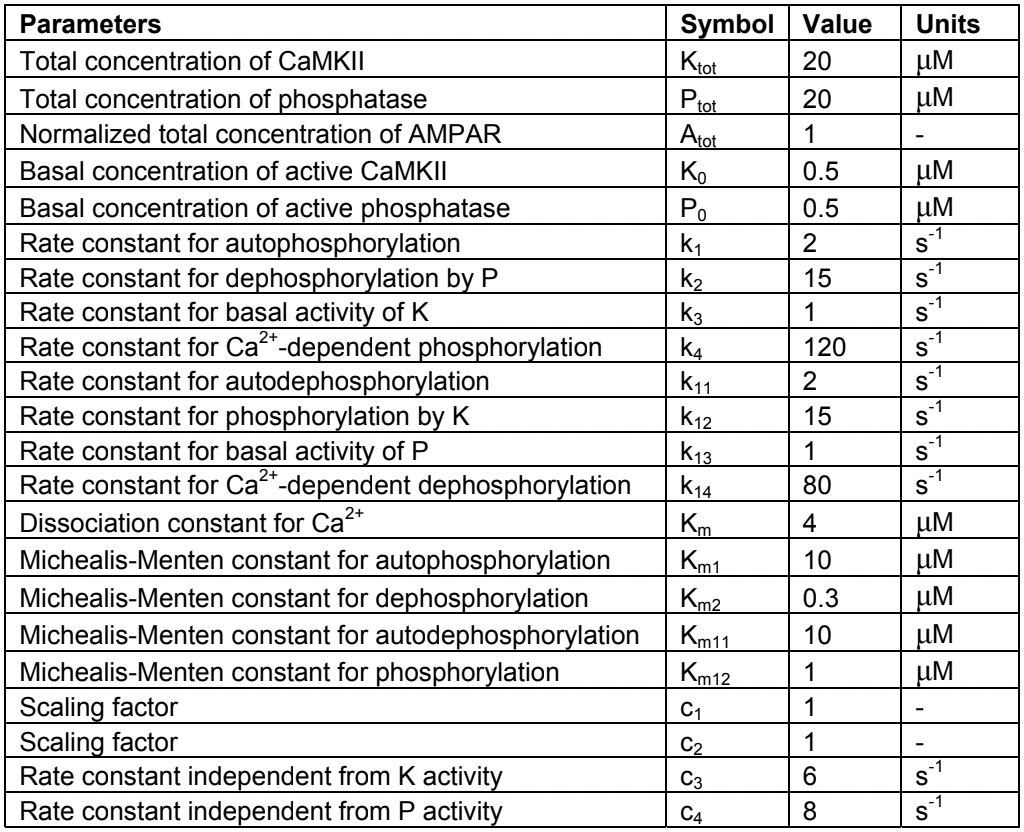
\includegraphics[width=.50\textwidth]{1.png}
    \end{center}
Under Pi and Lisman's setting, we have done some simulation to confirm its tristbality. We get the following result: The calcium impulse of $4\mu m$ last 2 $ms$, which induces LTP seen in the left column, while the calcium impulses of $2.2 \mu m$ last 2$ms$, which induces LTD seen in the right column
\begin{figure}[h]
    \centering
    \begin{minipage}[b]{0.45\textwidth}
        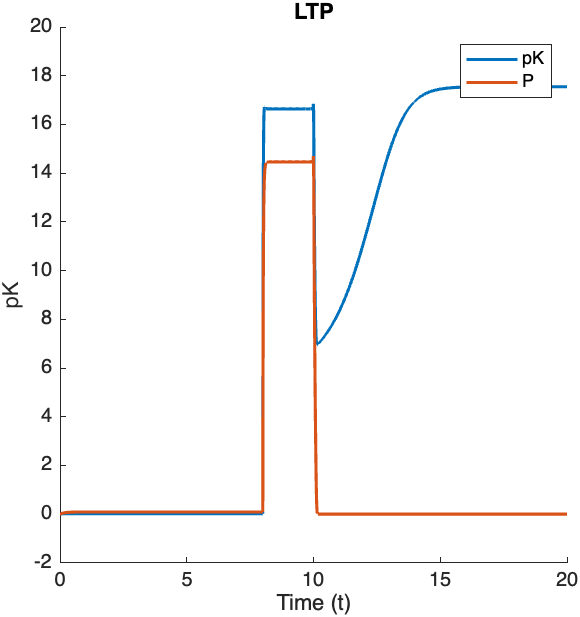
\includegraphics[width=\textwidth]{fig1.png}
        \caption{calcium impulse of $4\mu m$ last 2 $ms$}
        \label{fig:image1}
    \end{minipage}
    \hfill % or \hspace*{\fill} to have space between the two figures
    \begin{minipage}[b]{0.45\textwidth}
        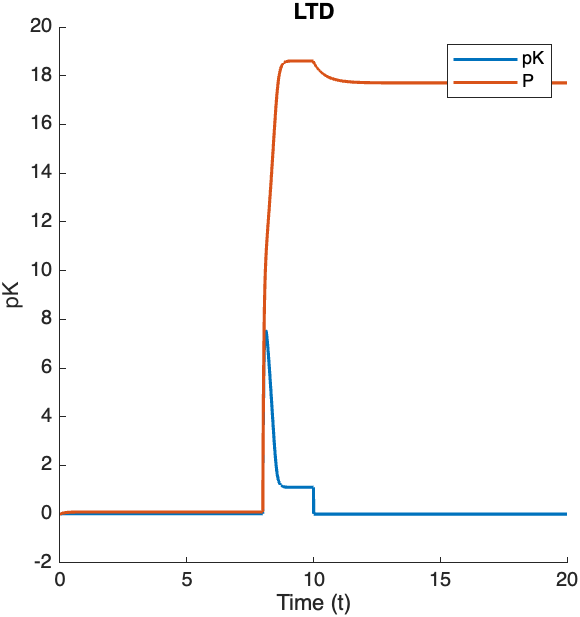
\includegraphics[width=\textwidth]{fig2.png}
        \caption{calcium impulses of $2.2 \mu m$ last 2$ms$}
        \label{fig:image2}
    \end{minipage}
\end{figure}
\linebreak
Here we can also use the AMPAR trafficking described in the Pi and Lisman's model. The reaction scheme is described as following:
$\begin{array}{c}
\ce{A_{int}} \underset{k_{22}}{\overset{k_{21}}{\rightleftharpoons}} \ce{A}
\end{array}$. The rate equation is \(
\frac{d}{dt}A = k_{21}A_{\text{int}} - k_{22}A,
\). The total AMPAR is assumed to be conserved \(A_{\text{tot}} = A + A_{\text{int}}\). Thus, we get following read-out at Figure 3.

\begin{figure}[h]
    \centering
    \begin{minipage}[b]{0.45\textwidth}
        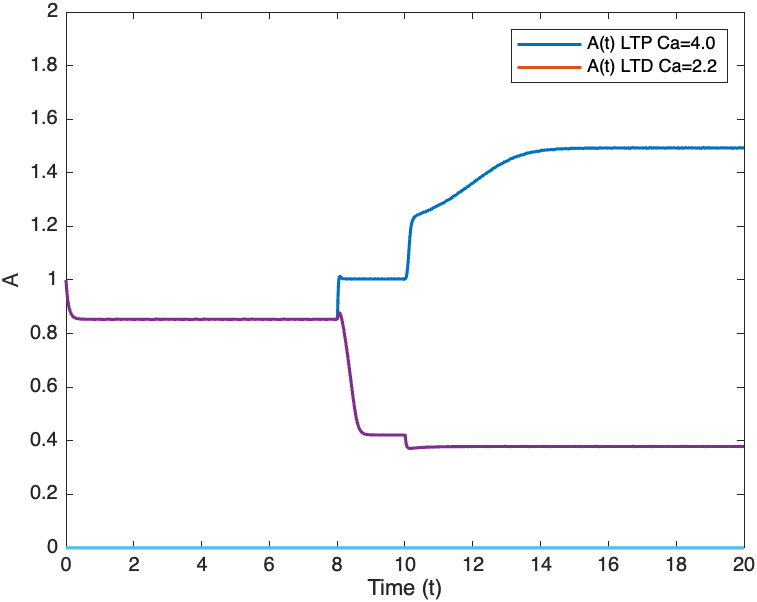
\includegraphics[width=\textwidth]{ampar.png}
        \caption{AMPAR read-out}
        \label{fig:image1}
    \end{minipage}
    \hfill % or \hspace*{\fill} to have space between the two figures
    \begin{minipage}[b]{0.45\textwidth}
        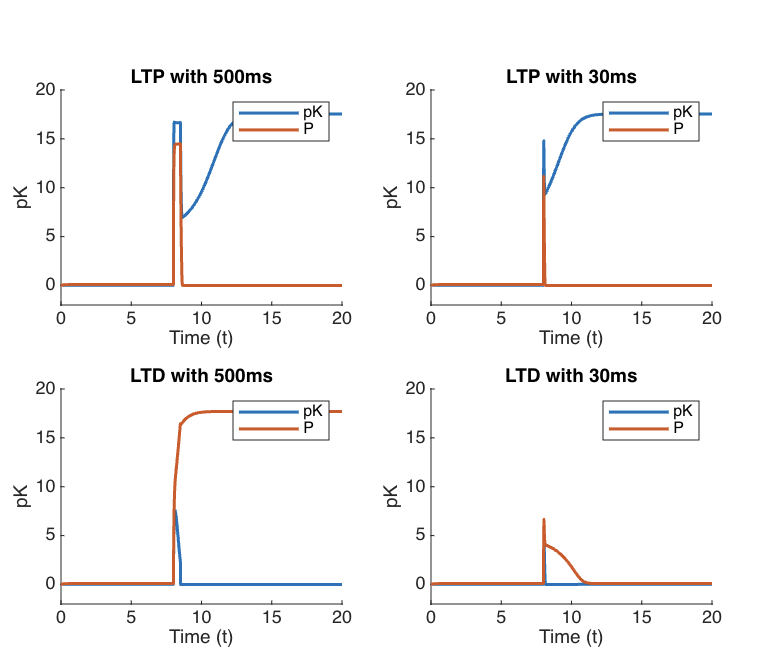
\includegraphics[width=\textwidth]{4plot.png}
        \caption{state caused by different time duration and impulse level}
        \label{fig:image2}
    \end{minipage}
\end{figure}

I also incorporate more experiment on different value of t and $Ca^{2+}$ to test its robustness, here is the result of Fig4. It confirm the tristability descirbed in Pi and Lisman's paper.
\newpage
To further test the robustness to small perturbation of this model, we apply following context: 0.4 $\mu m$ calcium impulse for 2 s) undergoes LTP by the second stimulation (4 $\mu m$ for 2 s). The third stimulation (2.2 $\mu m$ for 1.4 s) reverses the potentiated state back to basal level (depotentiation). The fourth (2.2 $\mu m$ for 2 s) and the fifth (2.93 $\mu$ for 2 s) stimulations induce and reverse LTD, respectively (dedepression).
\begin{figure}[h]
    \centering
    \begin{minipage}[b]{0.45\textwidth}
        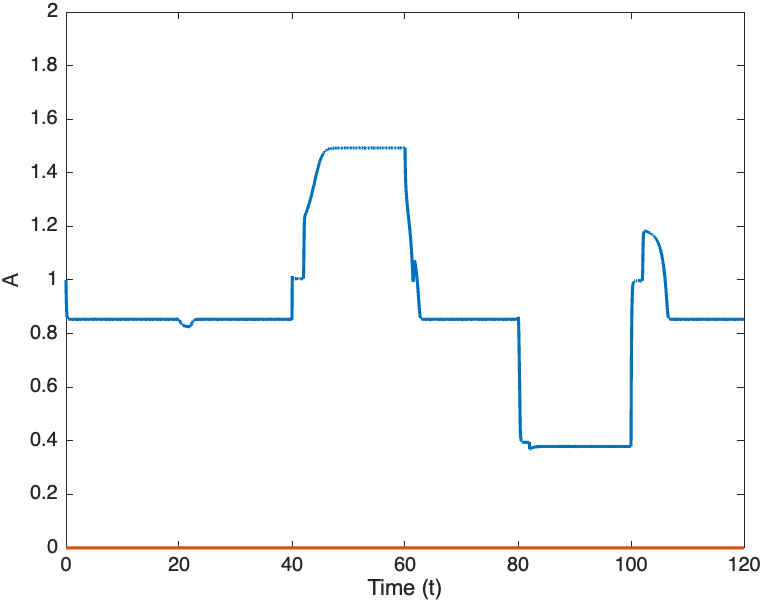
\includegraphics[width=\textwidth]{e.png}
        \caption{AMPAR read-out}
        \label{fig:image1}
    \end{minipage}
    \hfill % or \hspace*{\fill} to have space between the two figures
    \begin{minipage}[b]{0.45\textwidth}
        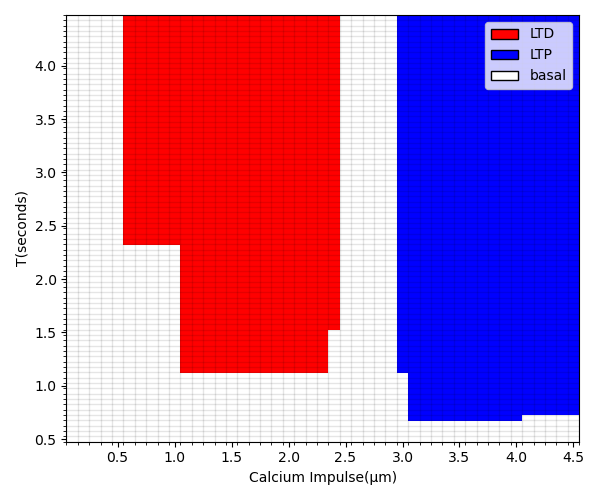
\includegraphics[width=\textwidth]{2.png}
        \caption{Phase plane of tristabile model}
        \label{fig:image2}
    \end{minipage}
\end{figure}\\
I have also done the grid search experiment to find that under Pi and Lisman's model, we have the following phase plane indicating the different combination of time and calcium flow resulting in different status LTD/P/basal.

\paragraph{1.2 Calcium dynamics in Carlson and Giordana's model}\mbox{}\\  
in Pi and Lisman setting, it assume the steady calcium flow, but in the realistic situation, we may expect calcium solved by dynamic system. Here we mainly follows Carlson and Giordana's model, but we will fix some of flaw that yet to be solved by them.\\
\linebreak
We first examine the calcium dynamics described by Carlson and Giordana. In this model, the author admit the importance of VDCC(Voltage-gated calcium channel) along with NMDARs' receptor as sources of \(Ca^{2+}\) influx.\\
1) The calcium current due to NMDARs is following:
\begin{equation}
I_{\text{NMDA}}(V, t) = P_0 \cdot G_{\text{NMDA}} \cdot \theta_1(t) \cdot \left[ I^f_{\text{glut}} e^{(t_{\text{glut}} - t)/\tau^f_{\text{glut}}} + I^s_{\text{glut}} e^{(t_{\text{glut}} - t)/\tau^s_{\text{glut}}} \right] \cdot H(V)
\end{equation}
where  we define $\theta_1(t)$ as \(\theta_1(t) = 
\begin{cases} 
0, & t < t_{\text{glut}} \\
1, & t > t_{\text{glut}}
\end{cases}\)\\
The term H(V) describes Mg$^{2+}$ unblock due to changes in the postsynaptic potential.
\begin{equation}
H(V) = (V_{\text{Ca}} - V) / \left(1 + ([\text{Mg}^{2+}] / 3.57) e^{-62V}\right)
\end{equation}
\linebreak
2 We define the VDCC current with following:
\begin{equation}
    I_{\text{VDCC}}(V, t) = G_{\text{VDCC}} \cdot \theta_2(V, t) \cdot (V_{\text{VDCC}} - V)
\end{equation}
where  we define \(\theta_2(V, t) =
\begin{cases}
1, & V > -30\,mV \text{ and } t_{\text{bpap}} + 2\,ms > t > t_{\text{bpap}} \\
0, & \text{otherwise}
\end{cases}\)\\
3)finally, combining (4) and (6), we could have the deferential equation of Calcium as following:
\begin{equation}
    \frac{dCa}{dt} = I_{\text{NMDA}} + I_{\text{VDCC}} - \frac{Ca - Ca_{\text{basal}}}{\tau_{\text{decay}}}.
\end{equation}

\begin{figure}[h]
    \begin{minipage}{.45\linewidth}
        \centering
        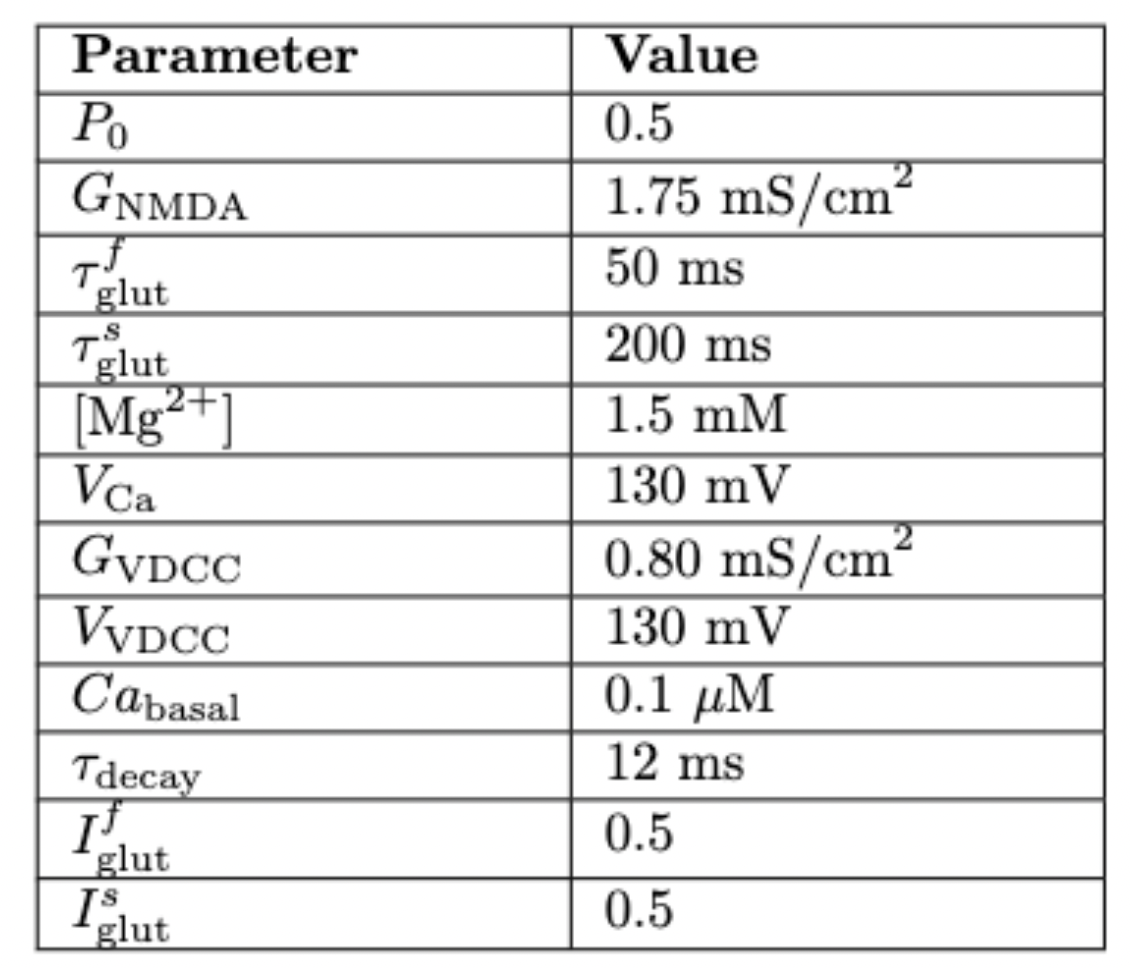
\includegraphics[width=.95\linewidth]{parameter_table.png}
        \caption{parameter table for calcium dynamics}
        \label{fig:fig4}
    \end{minipage}
    \hfill
    \begin{minipage}{.45\linewidth}
        \centering
        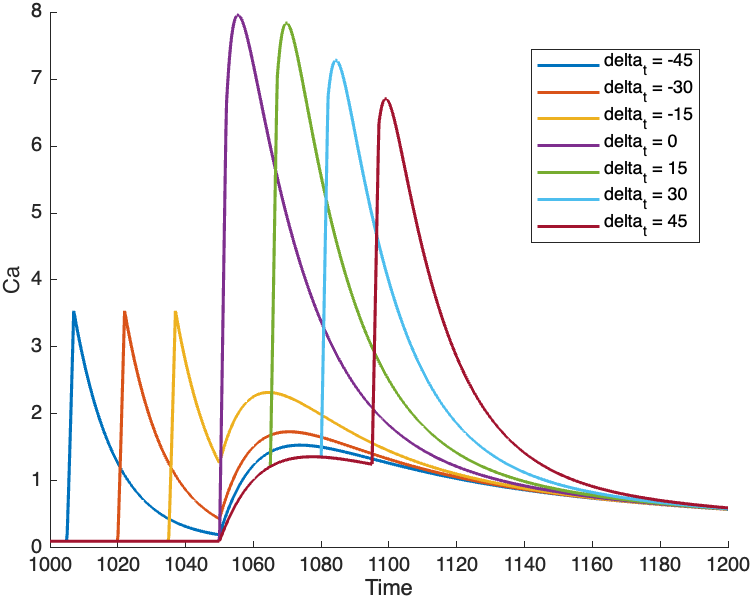
\includegraphics[width=.95\linewidth]{Ca.png}
        \caption{level of Ca respect to t}
        \label{fig:fig5}
    \end{minipage}
\end{figure}



We see the level of calcium as a function of t. The curve is different according to different $\delta t=t_{post}-t_{pre}=t_{bpap}-t_{glut}$. We simulate the calcium curve with different $\delta t$ respect to t in the figure 8.\\


 Under the previous defined model of calcium dynamic, we apply it in the Pi  and Lisman's model, and we get the following graph of level pK and P respect to t
 
\begin{figure}[h]
    \begin{minipage}{.45\linewidth}
        \centering
        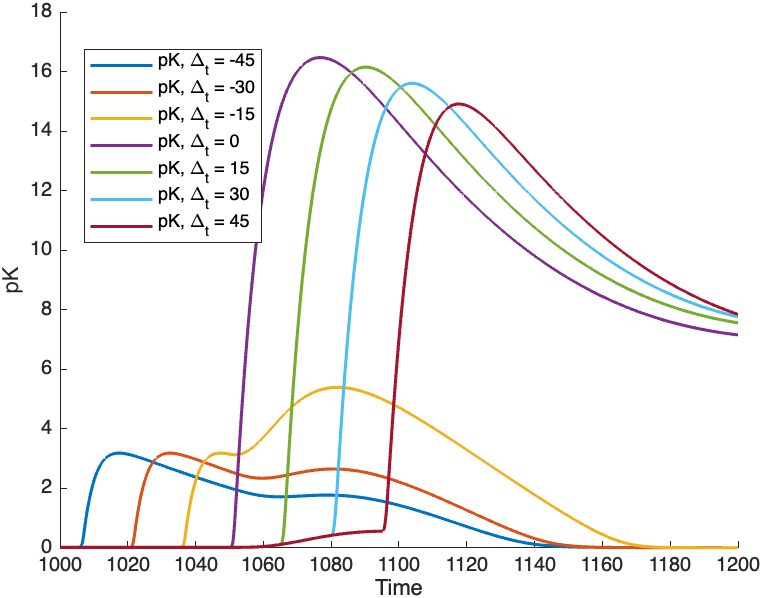
\includegraphics[width=.95\linewidth]{pK.png}
        \caption{level of pK respect to t}
        \label{fig:fig4}
    \end{minipage}
    \hfill
    \begin{minipage}{.45\linewidth}
        \centering
        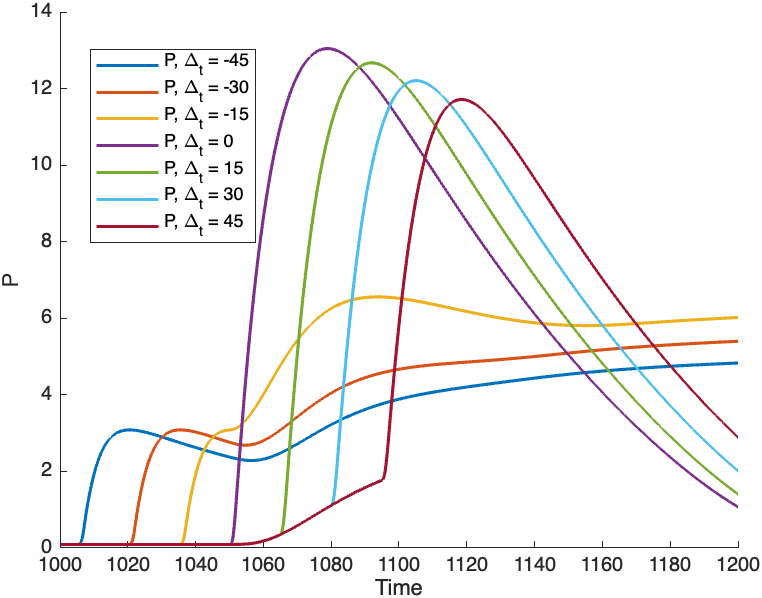
\includegraphics[width=.95\linewidth]{P.png}
        \caption{level of P respect to t}
        \label{fig:fig5}
    \end{minipage}
\end{figure}

According to the tristability protocal described in Pi\& Lisman's model. we get the following output \begin{table}[h]
    \centering
    \begin{tabular}{|c|c|}
    \hline
    $\delta t$ value & Direction \\
    \hline
    $0\text{ms}, 15\text{ms}, 30\text{ms}, 45\text{ms}$ & LTP \\
    \hline
    $-15\text{ms}, -30\text{ms}$ & LTD \\
    \hline
    $-45\text{ms}$ & Basal \\
    \hline
    \end{tabular}
    \caption{the result from the time difference in the set \{-45,-30,-15,0,15,30,45\}(ms)}
    \label{table:delta_t}
\end{table}


(comment: when $\delta t=-45ms$, it induce the basal, since the level of P eventually goes to basal level, which is not shown here )
\section{Multipair Pulse Induction}
while the Carlson and Giordana's model only shows successful LTP/LTD induction with only one spike pairing. Experimental results show that successful LTP/LTD induction requires many pulses (60) at a frequency of 1 Hz (Bi and Poo 1998; Wang et al. 2005). Now my next attempt is to use 60 pairs of induction.
        \begin{center}
        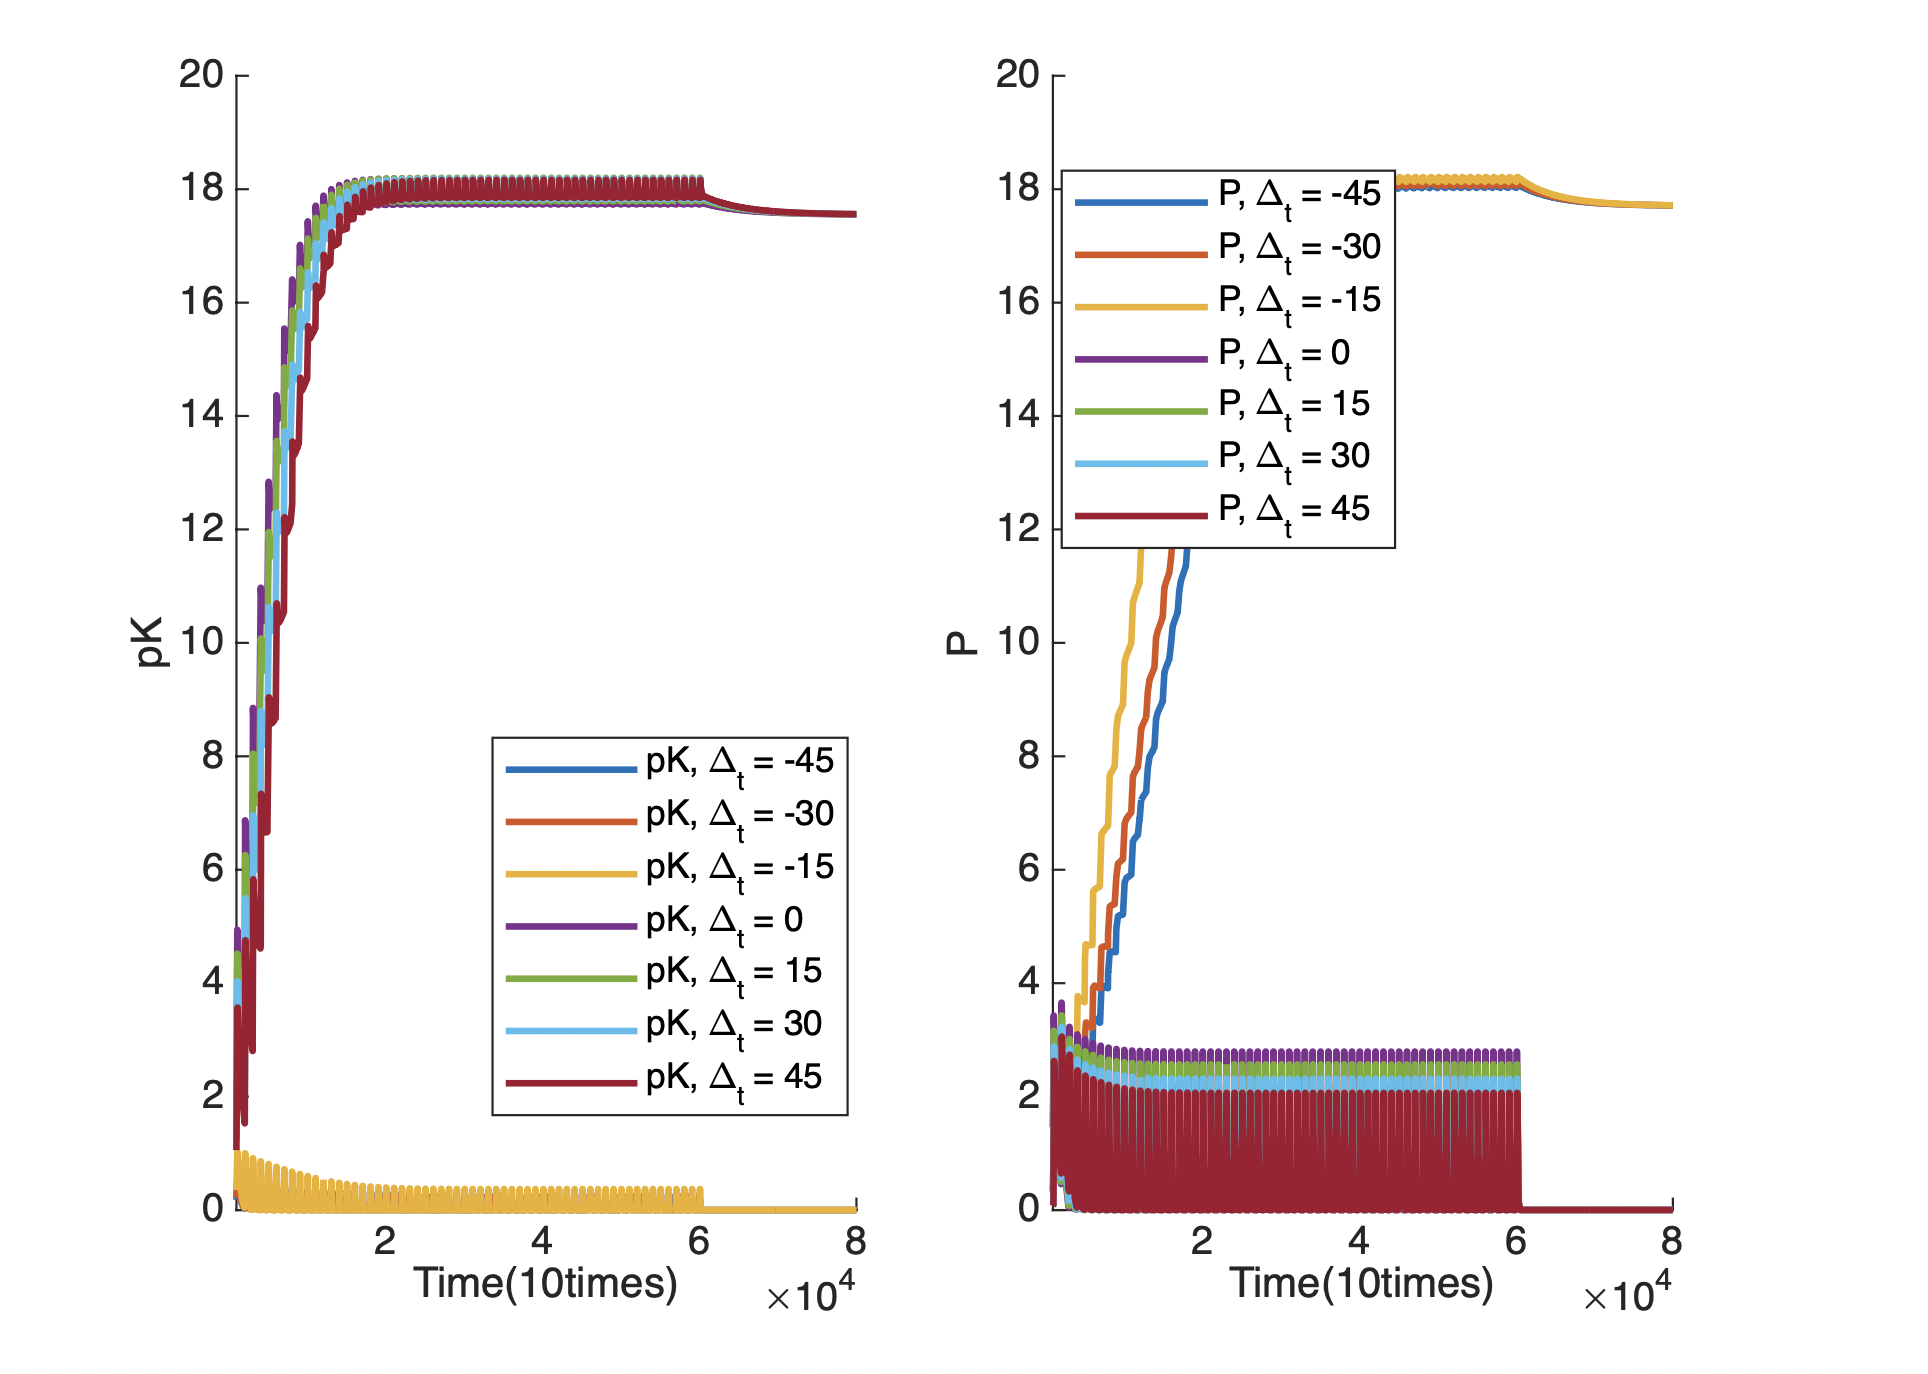
\includegraphics[width=.5\textwidth]{222.png}
    \end{center}
the left column is the result we from single spike induction corresponding to Carlson\&Giordana's paper, while the right column is our attempt that 60 pairs of spike induction

Under the multipair setting, i now present separated situation for the $\delta t$ in the following set $\{-45,-30,-15,0,15,30,45\}$
        \begin{center}
        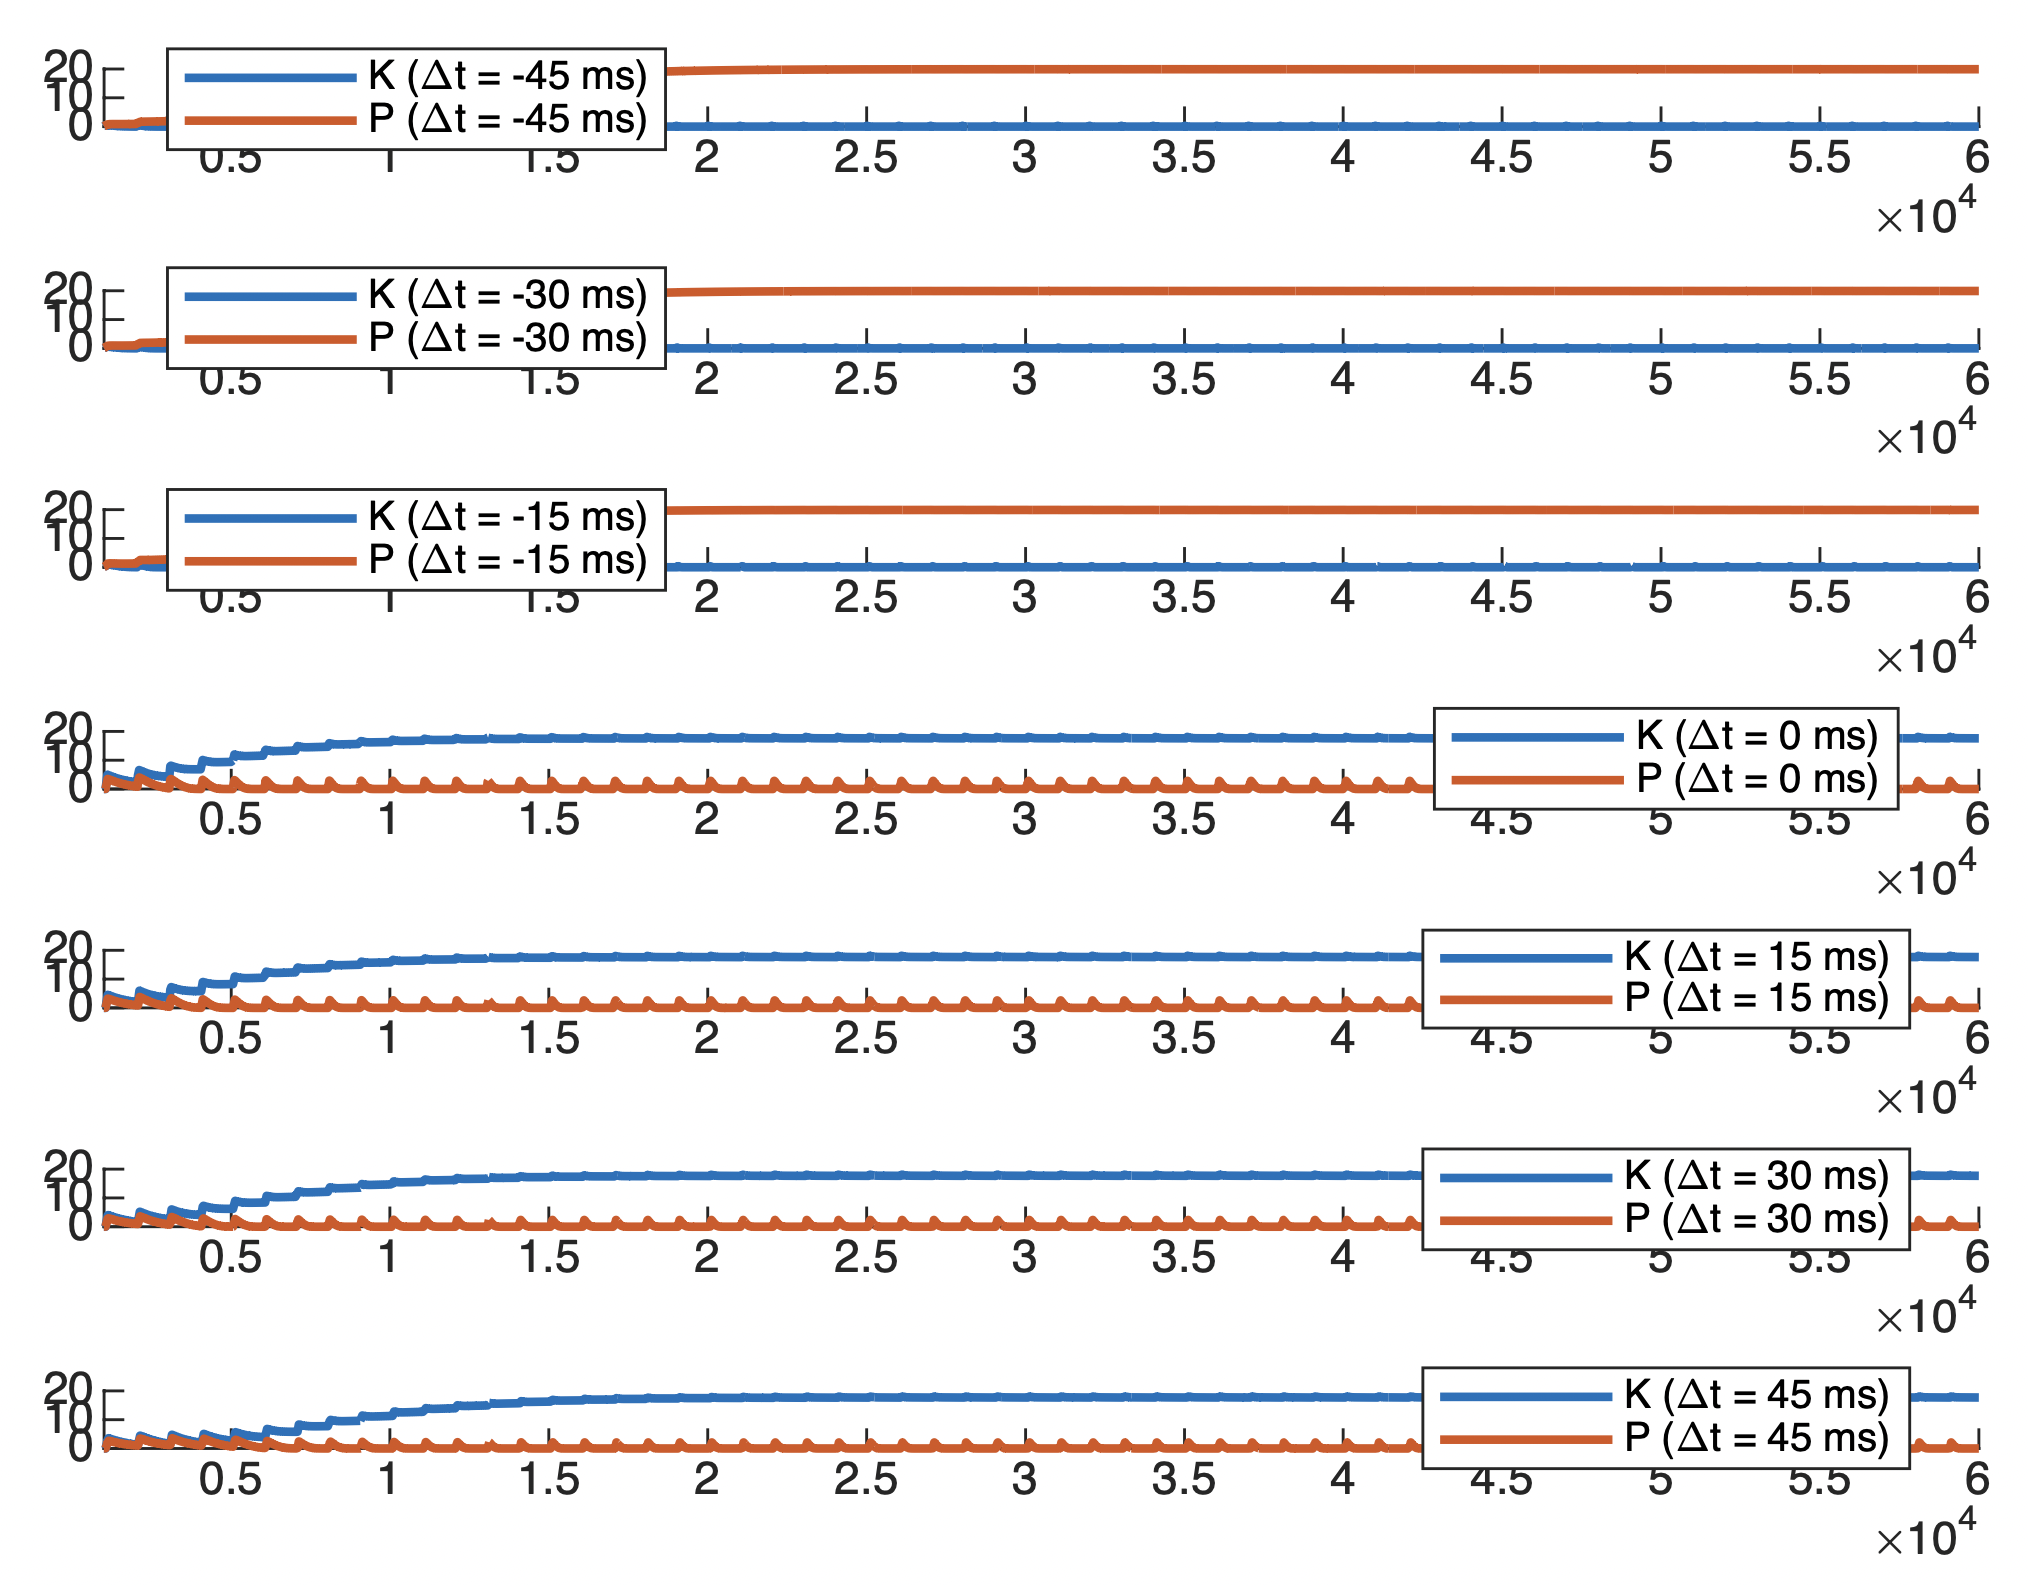
\includegraphics[width=.95\textwidth]{separated_plot.png}
    \end{center}
from this result, I make the grid to summary it.
\begin{table}[h]
    \centering
    \begin{tabular}{|c|c|}
    \hline
    $\delta t$ value & Direction \\
    \hline
    $0\text{ms}, 15\text{ms}, 30\text{ms}, 45\text{ms}$ & LTP \\
    \hline
    $-15\text{ms}, -30\text{ms},-45\text{ms}$ & LTD \\
    \hline
    \end{tabular}
    \caption{the result from the time difference in the set \{-45,-30,-15,0,15,30,45\}(ms)}
    \label{table:delta_t}
\end{table}


Now we consider the the extended time interval to [-500,500]
By the tristabile protocal described in Pi\&Lisman's model, we have following read out:
\begin{table}[h]
    \centering
    \begin{tabular}{|c|c|}
    \hline
    $\delta t$ value & Direction \\
    \hline
    $30\text{ms}, 45\text{ms}, 60\text{ms}, 75\text{ms}$ & LTP \\
    \hline
    \begin{tabular}{@{}p{5cm}@{}}
    $-30\text{ms}, -45\text{ms}, -60\text{ms}, -75\text{ms},$\\
    $-90\text{ms}, -100\text{ms}, -200\text{ms}, -300\text{ms},$\\
    $-400\text{ms}, -500\text{ms}, 90\text{ms}, 100\text{ms},$ \\
    $200\text{ms}, 300\text{ms}, 400\text{ms}, 500\text{ms}$
    \end{tabular} & LTD \\
    \hline
    \end{tabular}
    \caption{The result from the time difference in the set \\\{-500,-400,-300,-200,-100,-90,-75,-60,-45,-30,30,45,60,75,90,100,200,300,400,500\}(ms)}
    \label{table:delta_t}




Another illustration is shown in the following. As we can see, there are three problem that we may want to solve: 1) for the large $\delta t$ at both positive and negative part, we may want to see it goes back to basal. However, the current model only shows that for the large $\delta t$, it remains in LTD. 2)Also, the window of basal state for $\delta t$ around 0(turning from LTP to LTD) is too small. we want to see the intermidiate basal state.
\end{table}
           \begin{center}
        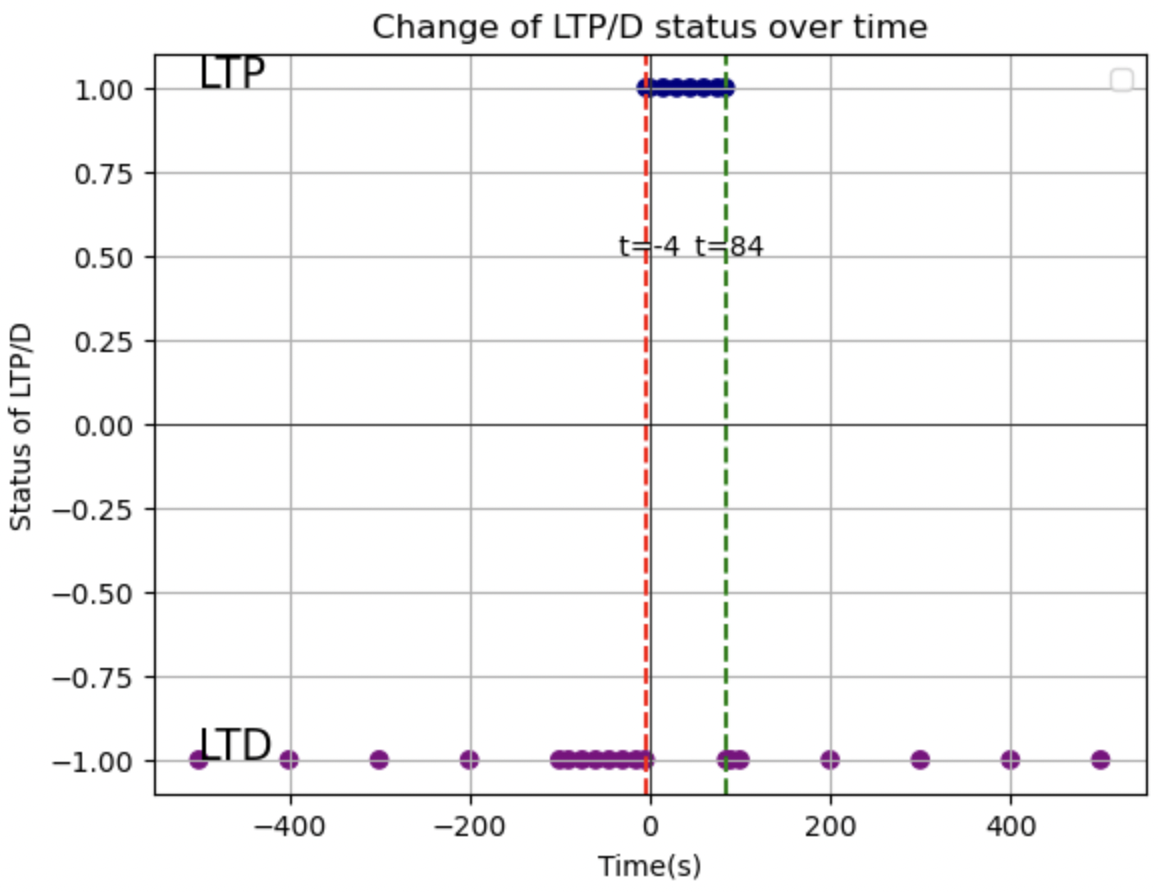
\includegraphics[width=.55\textwidth]{Carlson_Giordana_fig16.png}
    \end{center}

\newpage
\section{Parameter Tuning}
As described in the last section, we mainly want to deal with two thing 1)"blip" at LTD side 2) instability for large $\delta t$. Both of them indicates the calcium level in our model is too large calcium level. The way to reduce calcium level is by reduce the NMDA and VDCC current. The current setting for the parameter G$_{NMDA}$ and G$_{VDCC}$, according to Carlson and Giordana's, is 1.75 and 0.8. In previous section, we already found its flaw. My first attempt is that reduce both parameter to avoid the dominance of LTP in most case.\\
\linebreak
we first investigate into the case for the plot of P/pK/Ca with resepct to t in the first 3s under original parameter setting. 
\begin{figure}[ht]
    \centering
    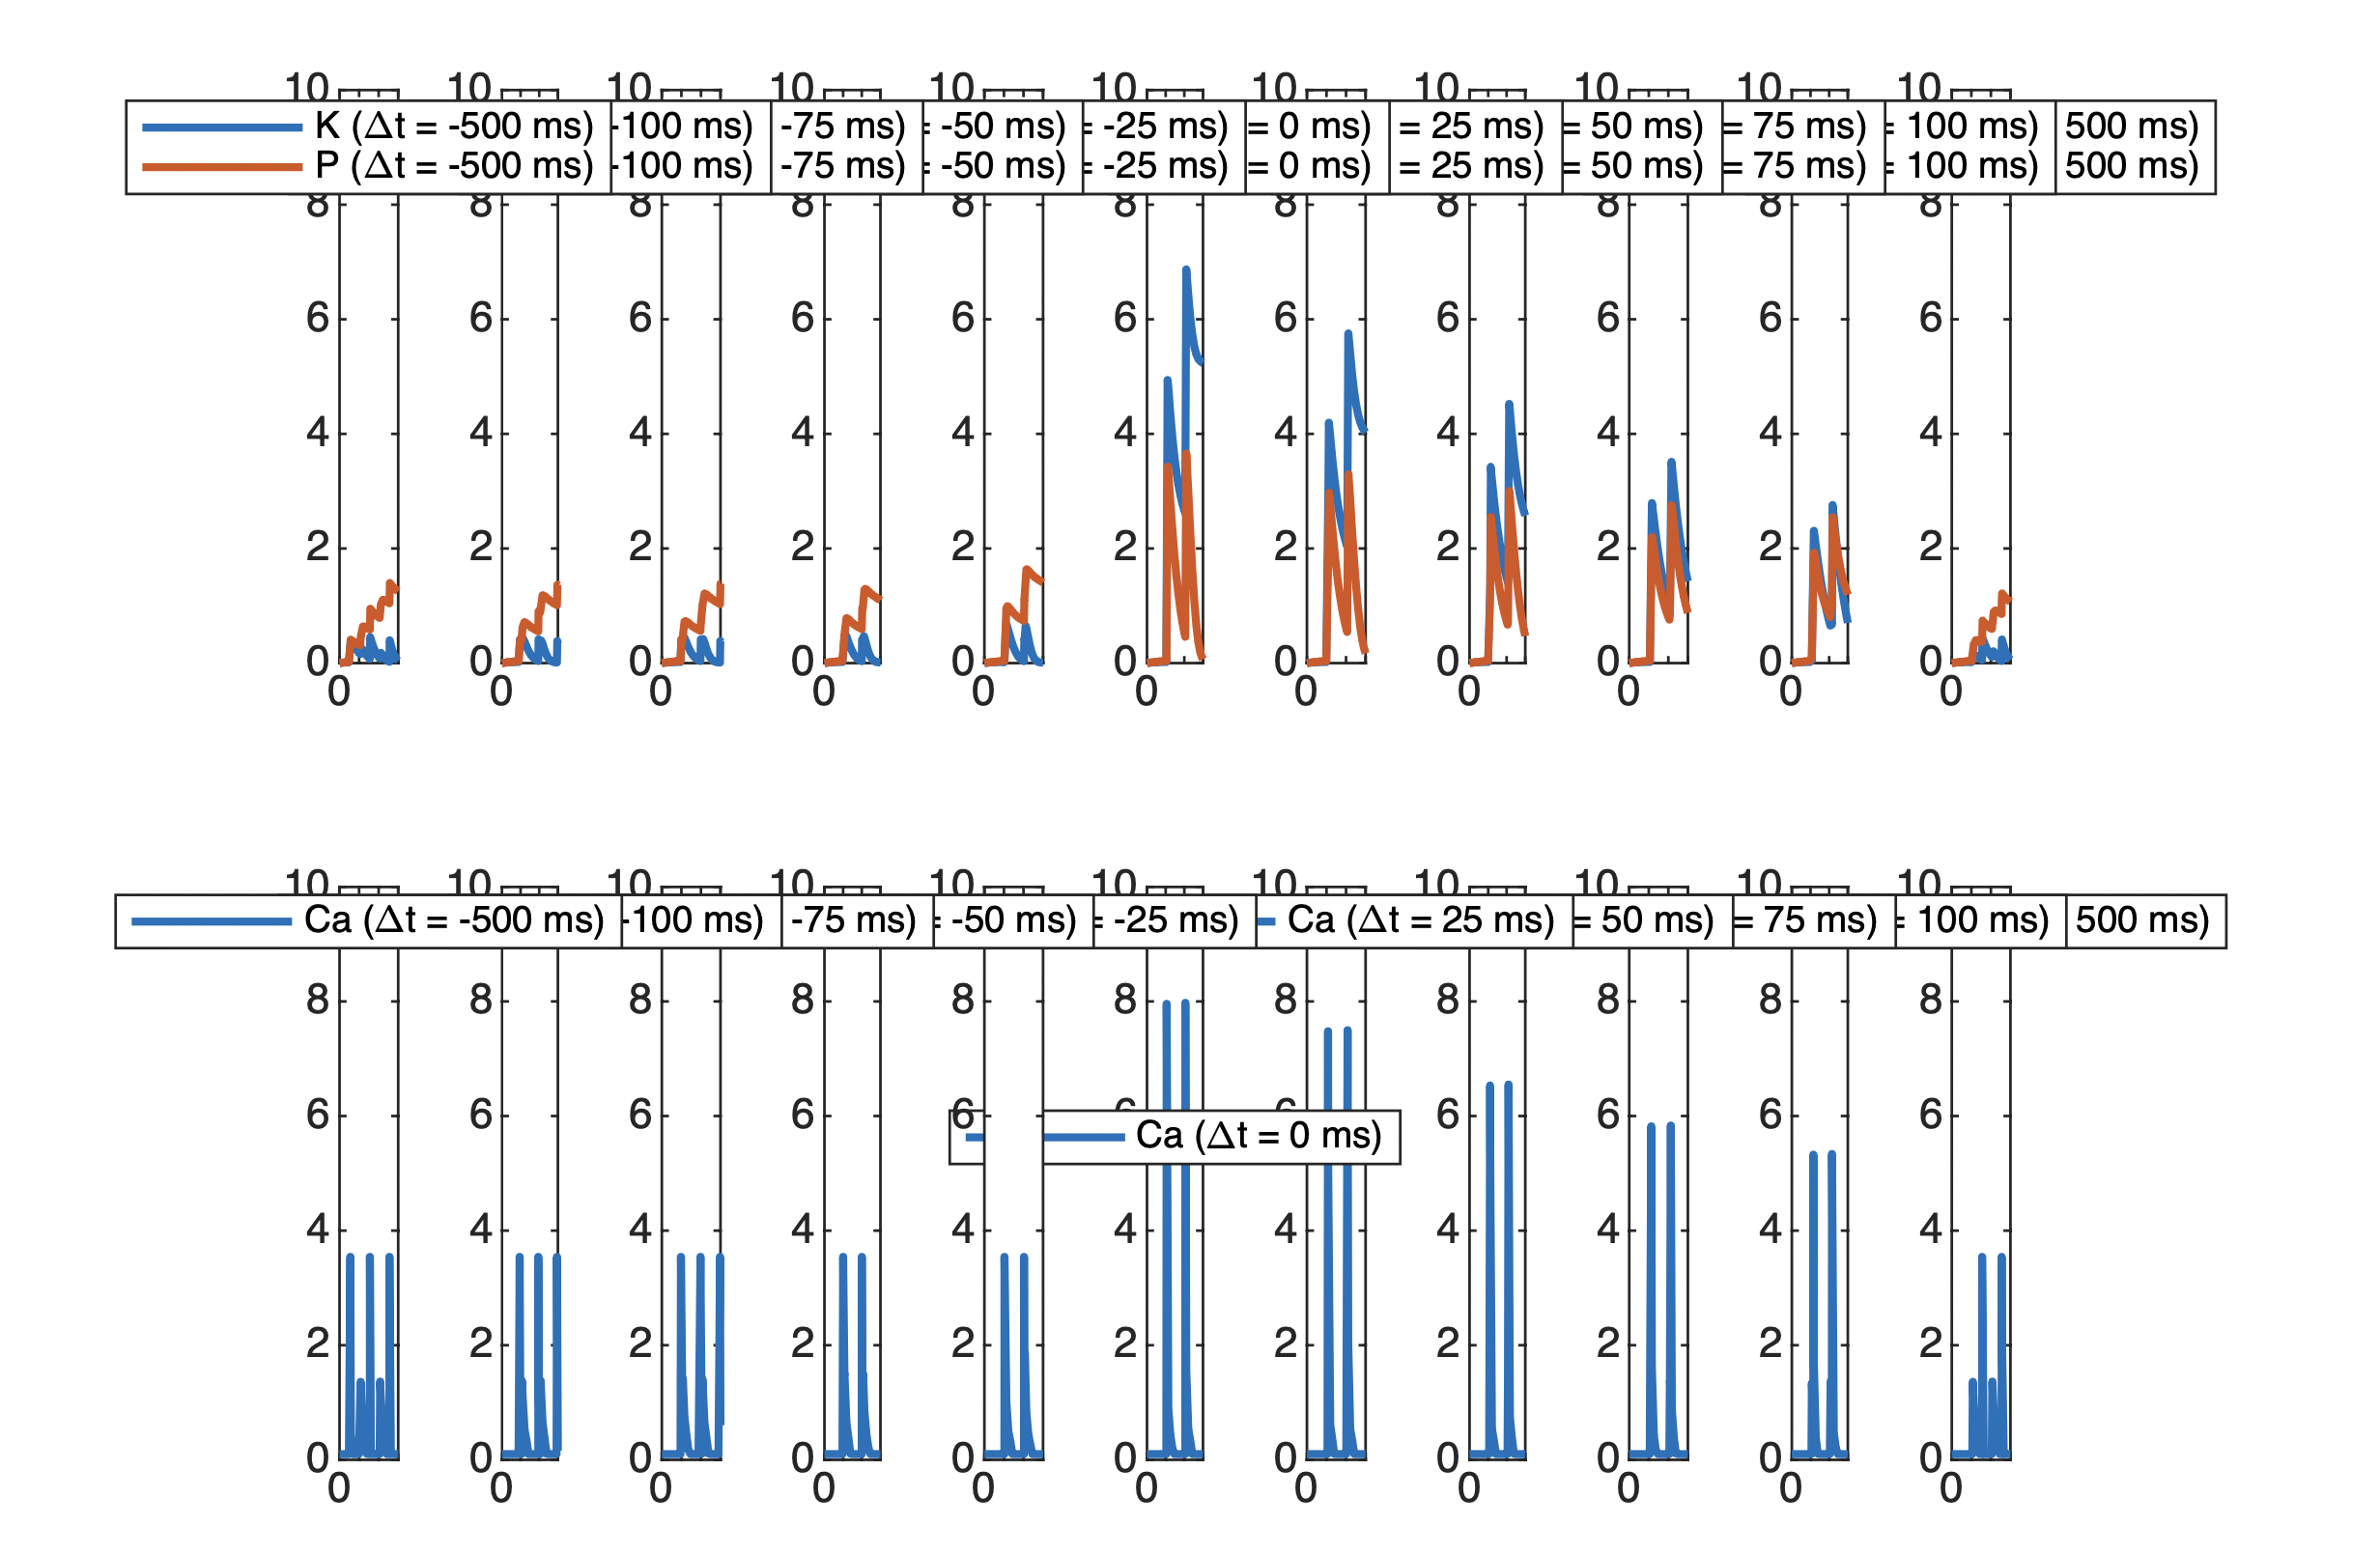
\includegraphics[width=.8\linewidth]{3.png}
    \caption{level of pK respect to t}
    \label{fig:fig4}
\end{figure}

\begin{figure}[ht]
    \centering
    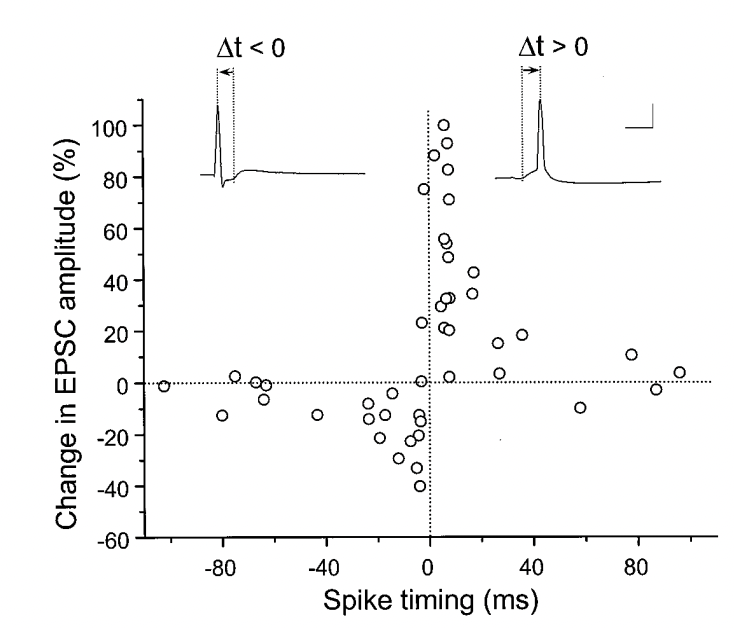
\includegraphics[width=.47\linewidth]{5.png}
    \caption{Bi and Poo's plot}
    \label{fig:fig5}
\end{figure}

As shown in Fugure 11, the first row display the plot of p/pK respect to t, and the second row indicates plot of Ca resepct to t. we found that the high level of Ca induce LTP, and it turned to LTD for lower level of calcium. In this case, we also may assume basal require less calcium flow than the LTD cases. Therefore, it confirm our previous finding that the calcium profile is too large. Therefore, my next step is to use grid search to roughly find some of potential candidate of the parameter for our model.\\
\linebreak
\textbf{Grid search result:}\\

My grid search is to take $G_{VDCC}$ from 0.2 to 0.8 with step size 0.1, and $G_{NMDA}$ from 0.8 to 1.7 with step size 0.1. We thus form the parameter pairs in our model. The criterion of for good candidate in our model is: 1) it has basal state around $\delta t~0ms$. 2)for some $\delta t>0$, we observe LTP and for some $\delta t $, we observe LTD. 3)for small enough/large enough $\delta t$, it goes back to basal. The figure 12 is the citation from Bi and Poo's previous experimental result. We want to have our model corresponding to the Bi and Poo's result, so i have designed criterion 1) 2) 3) to help me find the optical candidate.
\begin{figure}[ht]
    \centering
    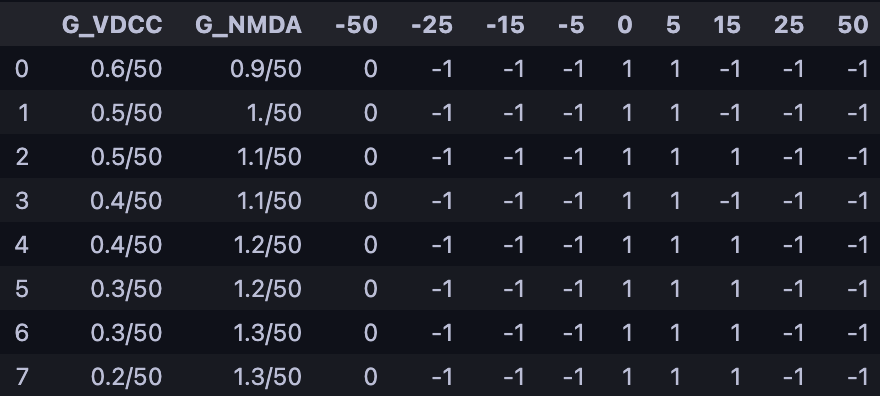
\includegraphics[width=.7\linewidth]{4.png}
    \caption{potential candidate from grid search}
    \label{fig:fig4}
\end{figure}\\
These are some of the result that could be seen as good candidate for the model, since it satisfy 1),2), but they all fail to admits 3). However, these set of parameter fails to go back to basal when $\delta t$ larger enough. In this case, they all remains to LTD state at $\delta t\in \{100,200\}$. We are not satisfy with this result, since it is deviate what we expect to see at large $\delta t$. Thus, my next step is to choose one of candidate from this, and further adjust parameter. \\In this case, we choose the parameter set $G_{VDCC}$=0.30,$G_{NMDA}$=1.30 as starting point for investigation. The premier goal is to ensure the model goes back to basal large $\delta $t (for exaple: at least $\delta t>100s$)
\begin{figure}[h]
    \centering
    \begin{minipage}[b]{0.45\textwidth}
        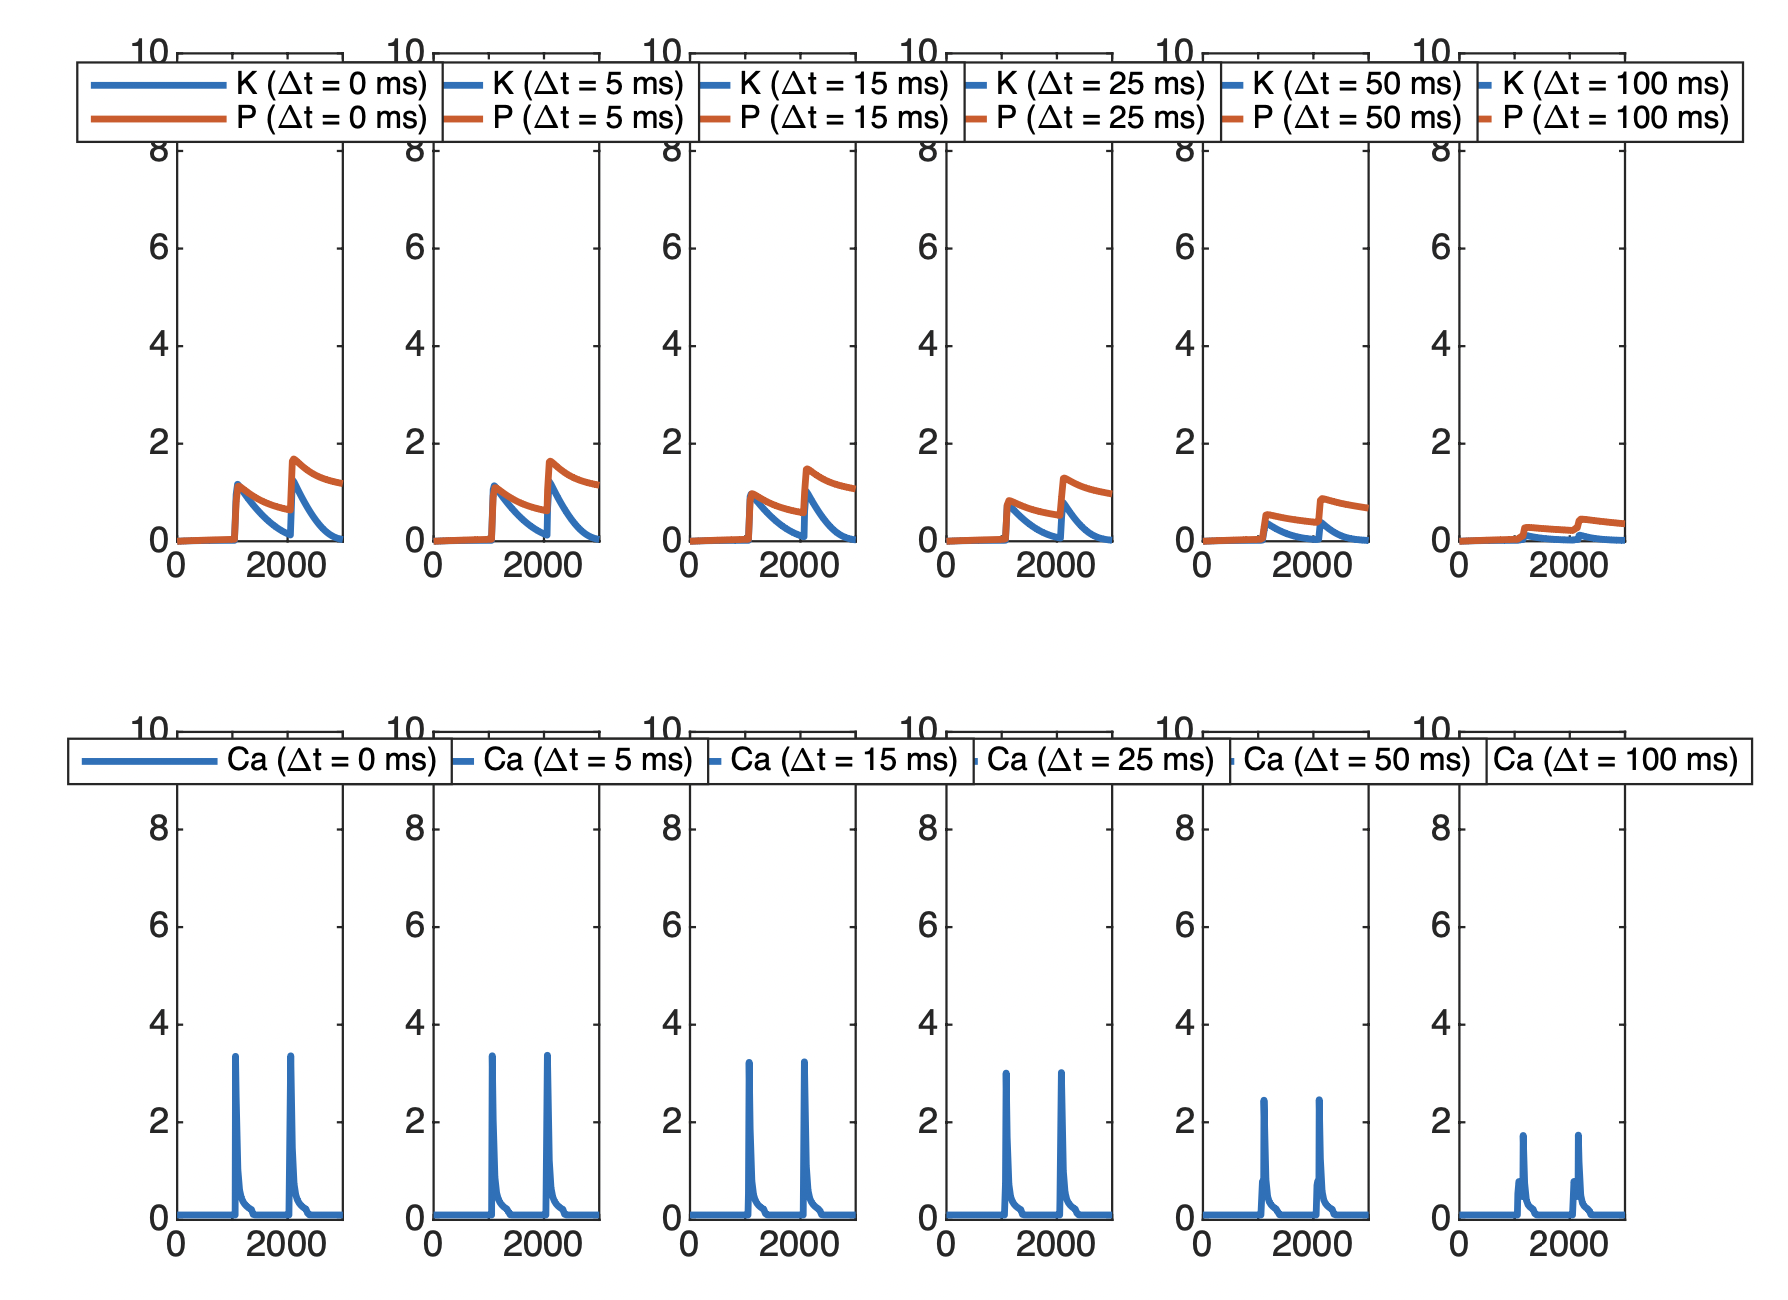
\includegraphics[width=1.1\textwidth]{0.1.png}
        \caption{$G_{NMDA}=0.2,G_{VDCC}=1.3$}
        \label{fig:image1}
    \end{minipage}
    \hfill % or \hspace*{\fill} to have space between the two figures
    \begin{minipage}[b]{0.45\textwidth}
        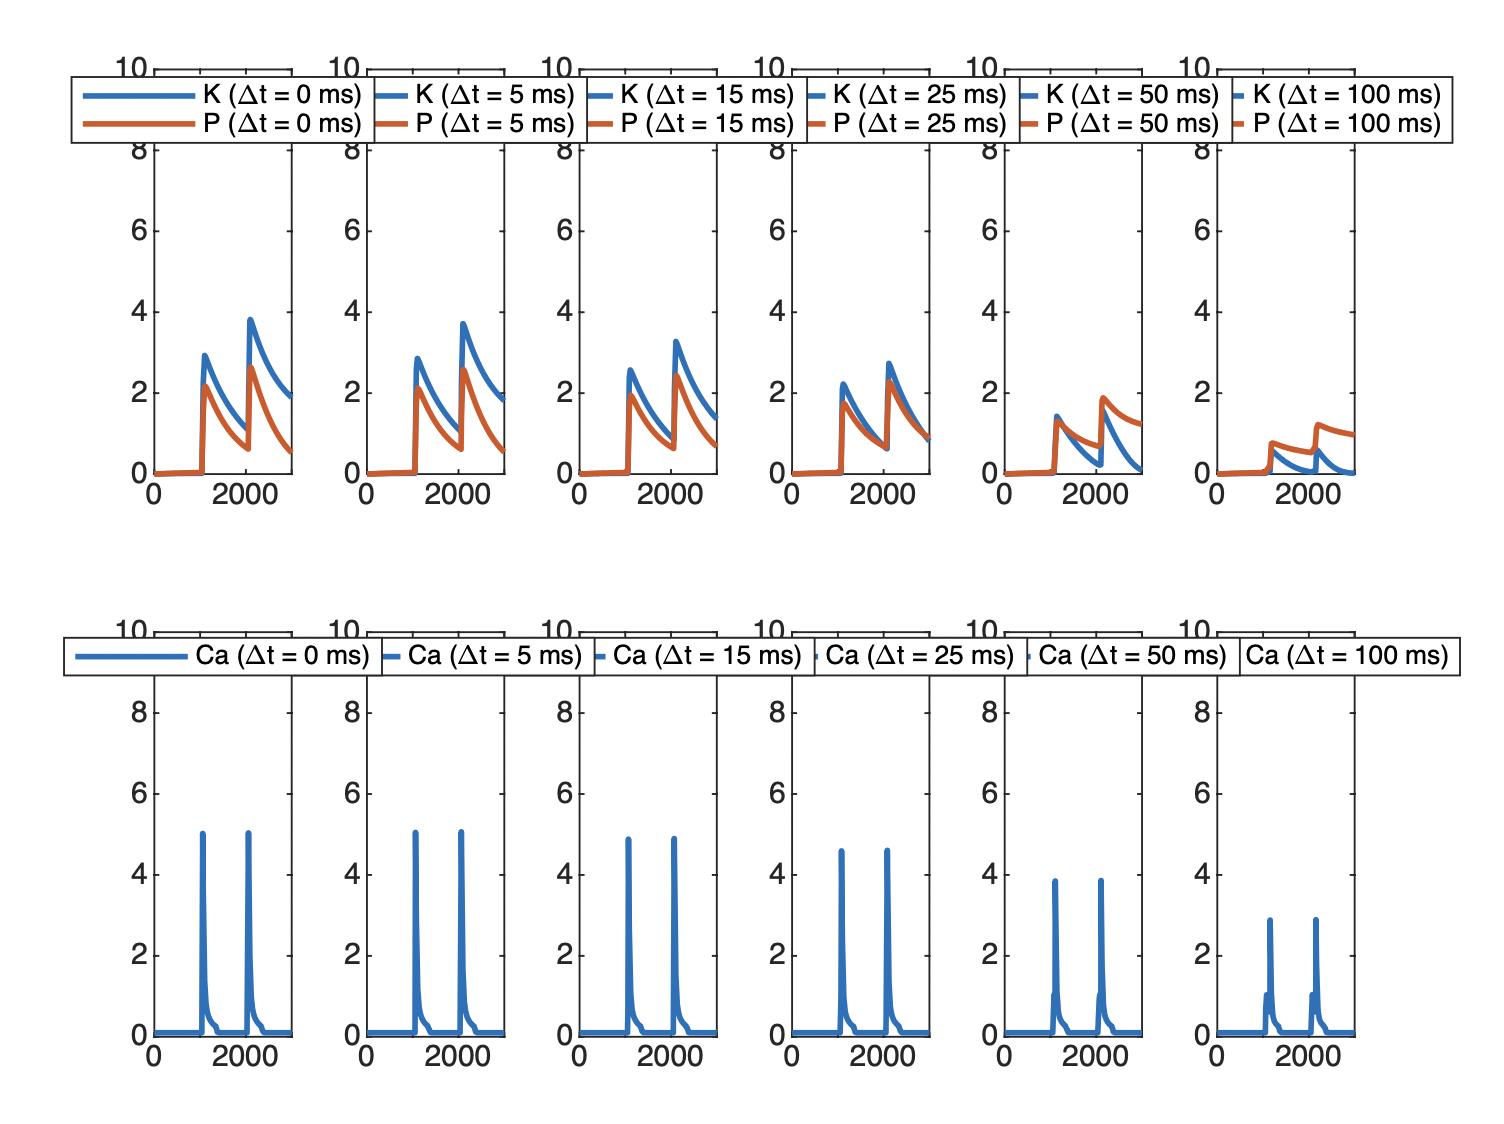
\includegraphics[width=\textwidth]{0.3.png}
        \caption{$G_{NMDA}=0.1,G_{VDCC}=0.95$}
        \label{fig:image2}
    \end{minipage}
\end{figure}\\
After adjusting the parameter, we found that when $G_{NMDA}=0.1,G_{VDCC}=0.95$, we ensure that the model stable basal for $\delta t$ larger than certain value in $[50,100]$. In this case, we goes back to test if it satisfy 3 criterion i have made before. we found that it stays at basal for large enough $\delta t$ and small enough $\delta t$, so 3) is met. However, We have also found that for the $\delta t\in [-50,50]$, it all induce LTD and fail to induce LTP. This is the result that the calcium level is small. We need to expect larger caicium level to see the LTP, but we may not guarantee for the positive part, it will stay basal.\\ Therefore, we may conclude that the window of parameter for observing LTP is quite small. Since in this model, small change in calcium level could result in LTP to LTD. Here is the example, $G_{NMDA}=0.6,G_{VDCC}=0.9$, for $\delta t=5$, it is LTD. For $\delta t=15$, it turns to LTP. We can observe in this case, the calcium level for these two stats are really close.
\begin{figure}[ht]
    \centering
    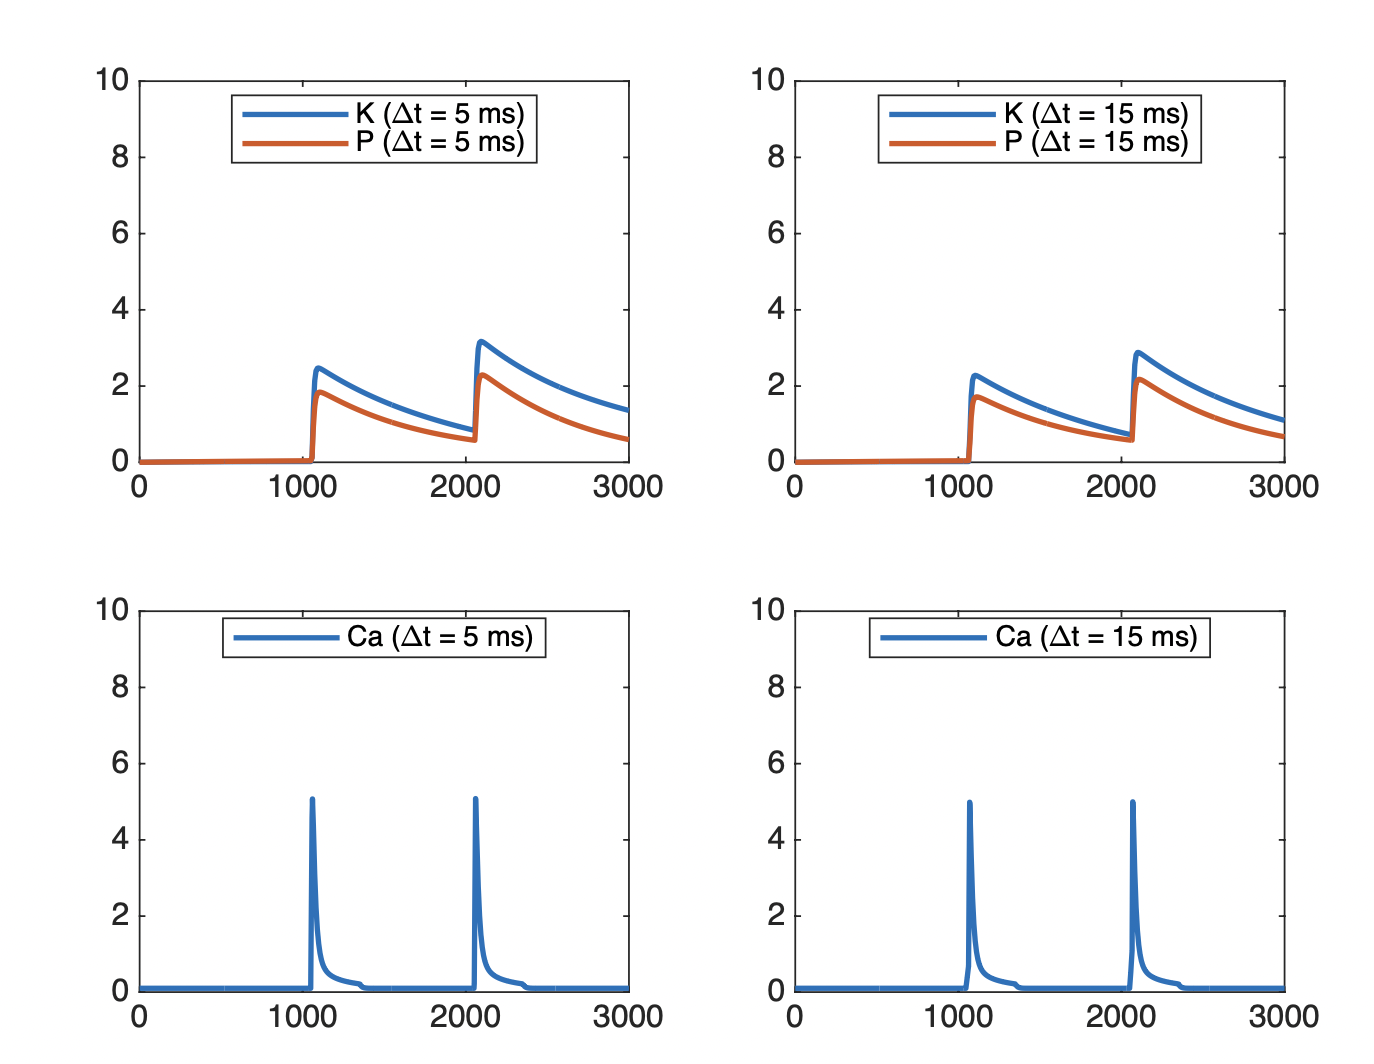
\includegraphics[width=.6\linewidth]{0.6.png}
    \caption{$G_{NMDA}=0.6,G_{VDCC}=0.9$}
    \label{fig:fig4}
\end{figure}\\
since this model is so sensitive to subtle changes in parameter, which means the parameter ranges without the 'blip' seem to be so narrow and delicate, it is not a good biophysical model. Therefore, for now, we can leave the existence of blip as it is, and the STDP curve is shown in the Figure 19. Then, i may try to incorporate "compact open state" which will increase the dynamical system from 2 dim to 3 dim in my model. At the same time i will use higher performance computing resource to grid search with finer grid to find the parameter set that eliminate the "blip" in the model.
\begin{figure}[ht]
    \centering
    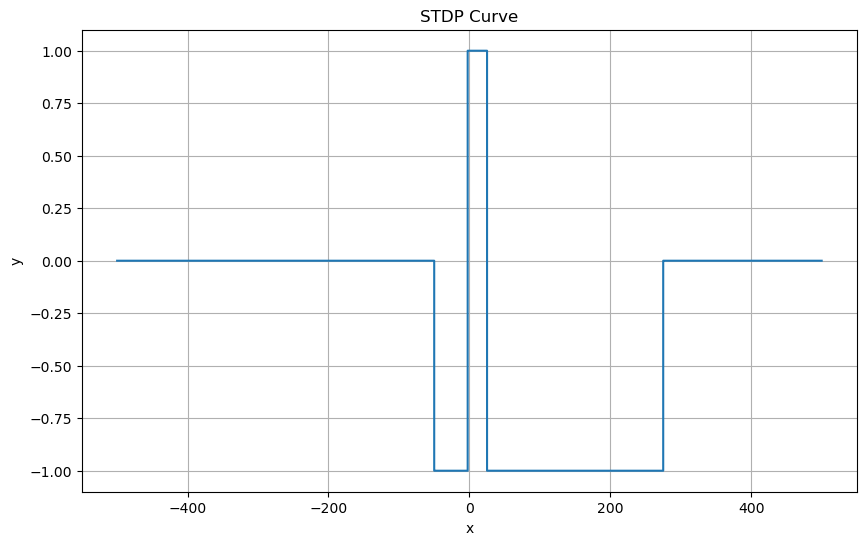
\includegraphics[width=.5\linewidth]{STDP.png}
    \caption{STDP curve}
    \label{fig:fig4}
\end{figure}\\


\section{compact open state}
In this section, i incorporate compact open state in my model. I firstly started with the simplified version of compact state, and the system now become:

\begin{equation}
\left\{
    \begin{aligned}
        \frac{d}{dt}pK &= k_1 \frac{K}{K_{m1} + K}pK - k_2 \frac{pK}{K_{m2} + pK}(P + P_0) + k_3K_0 + k_4 \frac{Ca^4}{K_{m4}^4 + Ca^4} K\\
        \frac{d}{dt}P &= k_{11} \frac{pP}{K_{m11} + pP}P - k_{12} \frac{P}{K_{m12} + P}(pK + pK_0) + k_{13}P_0 + k_{14} \frac{Ca^3}{K_{m}^3 + Ca^3}pP,\\
        \frac{dC}{dt} &=-\mu C+\nu K
    \end{aligned}
\right.
\end{equation}

We aim to make $\mu$ Ca-dependent and make $\nu$ pK-dependent to improve our model. We use following to model $\mu$ and $\nu$:
\[
\mu(\text{Ca})=\text{base} \mathbbm{1}_{\text{Ca}<\text{threshold}}+\text{height}\mathbbm{1}_{\text{Ca}\geq\text{threshold}}
\]
\[
\nu(\text{{pK}}) = \nu \cdot\left( \frac{\beta}{1 + \lambda \cdot \text{{pK}}}  + 1 - \beta\right)
\]
If we set \(\text{base}=1.5, \text{threshold}=0.2, \text{height}=40, \beta=0.9, \lambda=\frac{1}{5},\nu=0.5\). We get the following phase diagram:
\begin{figure}[ht]
    \centering
    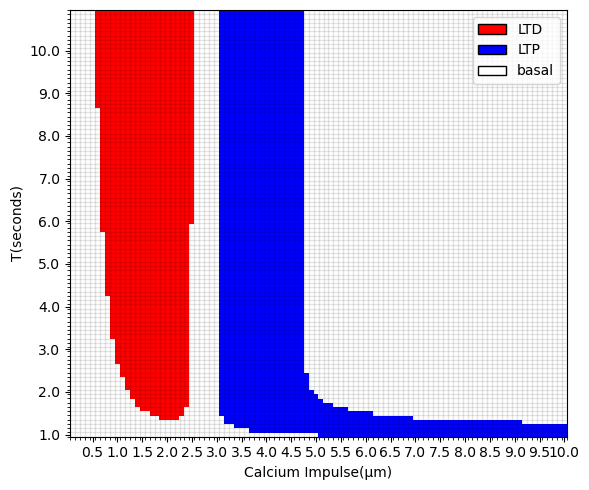
\includegraphics[width=.75\linewidth]{[1.5,0.2,40].png}
    \caption{STDP curve}
    \label{fig:fig4}
\end{figure}\\
The result is somehow desired, and we want to smooth the step function in $\mu$ to improve our model....

\newpage
\section{parameter tuning}
In this section, i will summarize the parameter we are currently working on with its function and related result.
\subsection{a}
a is defined as this way:\[
k4_{\text{new}}=a\cdot k4_{\text{original}}, k14_{\text{new}}=a\cdot k14_{\text{orginal}}
\]
the parameters "K4, K14", the reaction rate of calcium-induced phosphorylation of CaMKII and calcium-induced dephosphorylation of PP, function analogously as the "sensitivity" to the external calcium stimulus.\\
Originally, $k4=12,k14=8$, we are now timing the parameter "a" to make this system less sensitive to calcium impulse. Most extreme case: $a=0$, then biochemical system will not be responsive to the external calcium impulse\\
\begin{minipage}{\textwidth} % Full width for the first plot
    \centering
    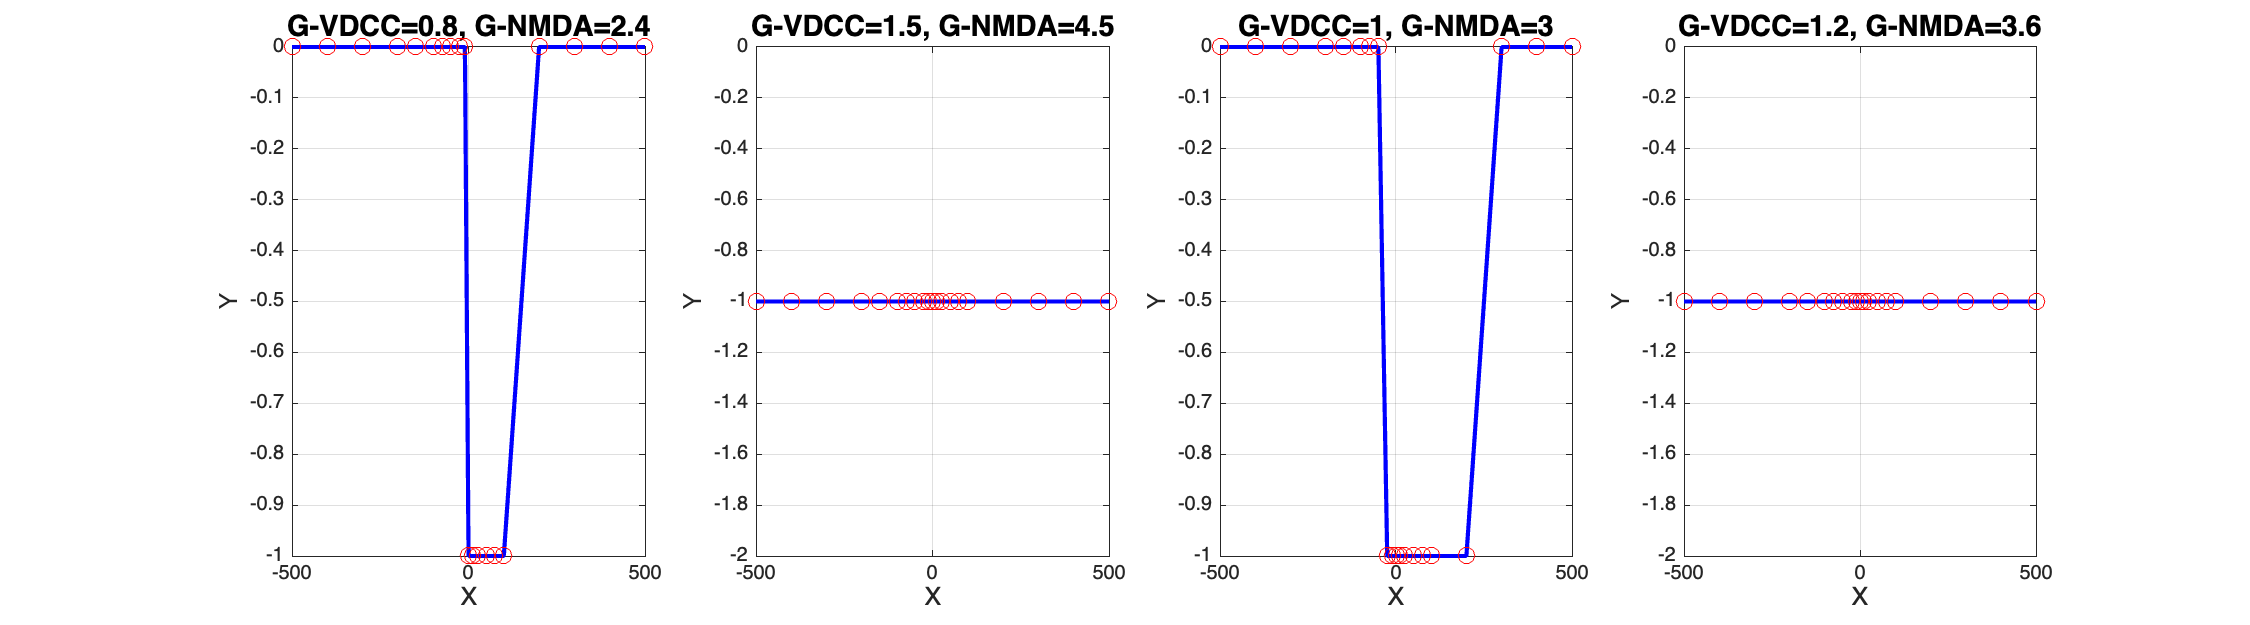
\includegraphics[width=0.8\textwidth]{a=0.1.png} % Change 'a=0.1.png' to your file name
    \captionof{figure}{ \( a = 0.1 \)}
    \label{fig:a0.1}
\end{minipage}

\vspace{0.5cm} % Space between plots

% Second plot
\begin{minipage}{\textwidth} % Full width for the second plot
    \centering
    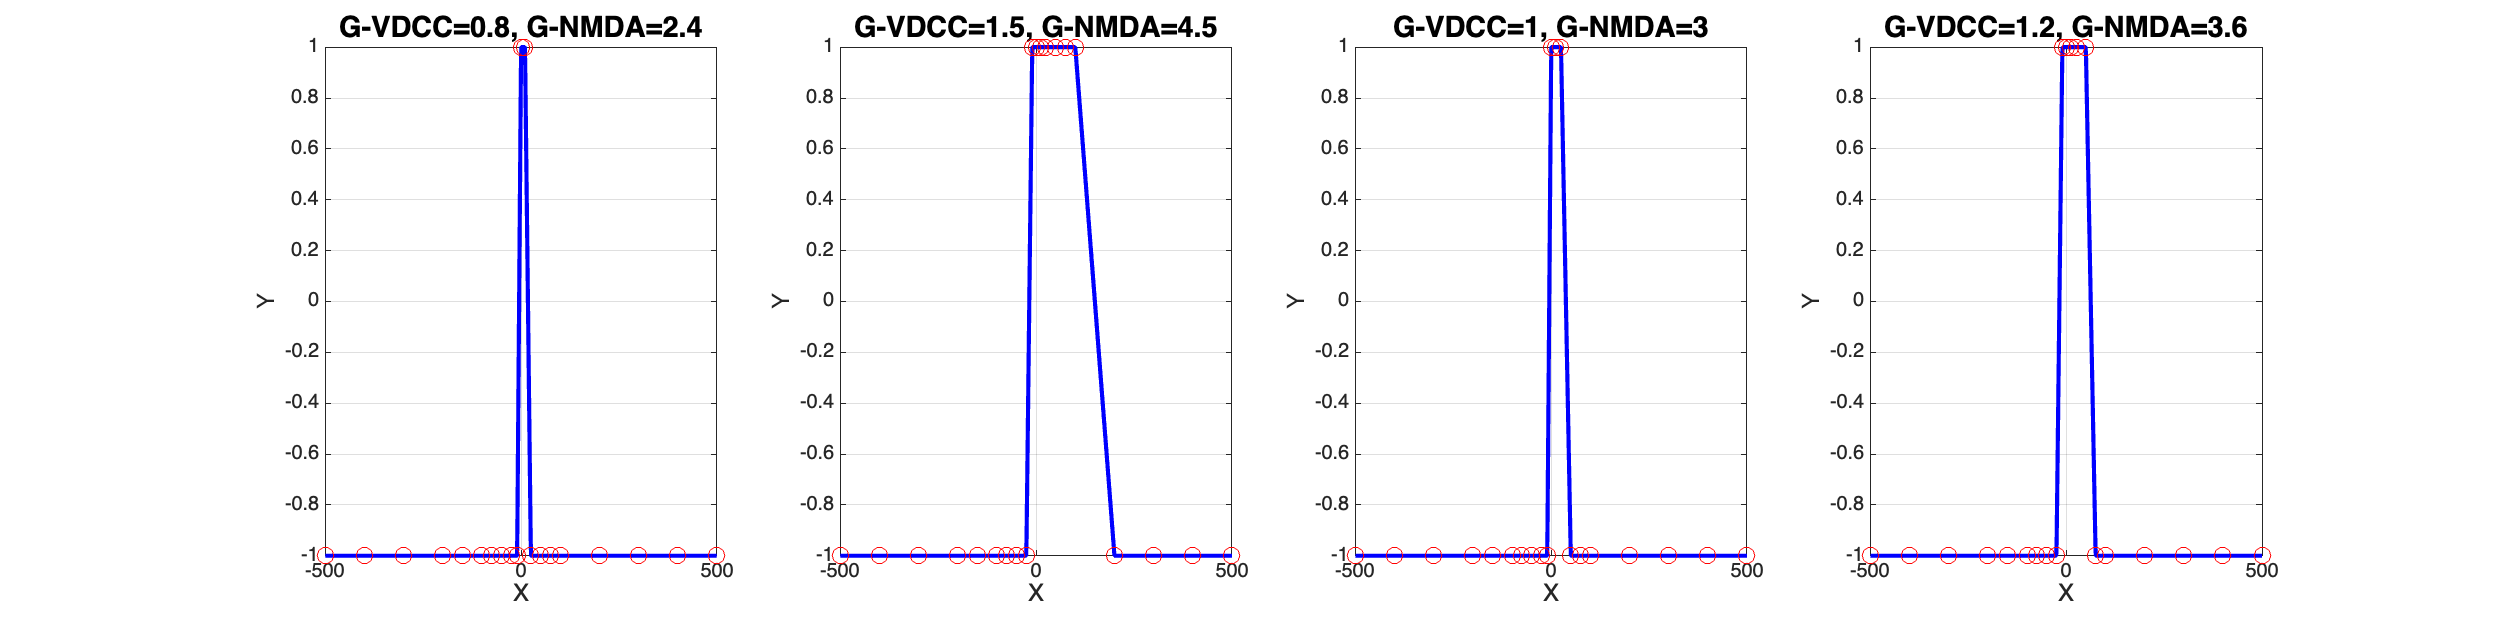
\includegraphics[width=0.8\textwidth]{a=0.25.png} % Change 'a=0.25.png' to your file name
    \captionof{figure}{ \( a = 0.25 \)}
    \label{fig:a0.25}
\end{minipage}

\vspace{0.5cm} % Space between plots

% Third plot
\begin{minipage}{\textwidth} % Full width for the third plot
    \centering
    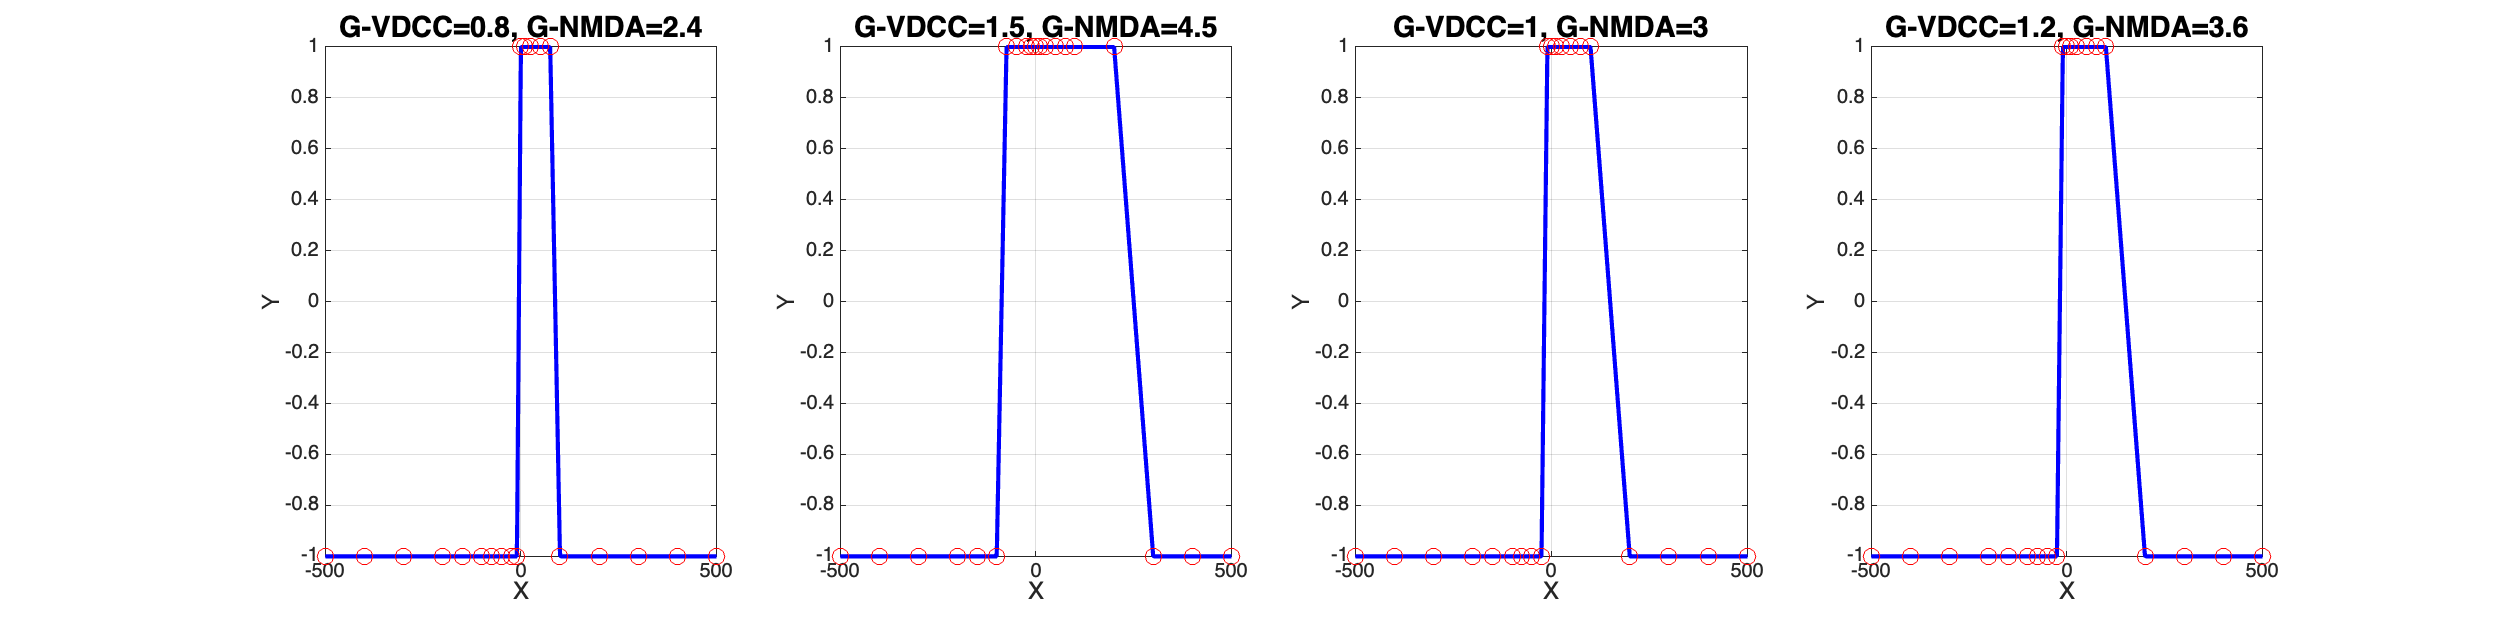
\includegraphics[width=0.8\textwidth]{a=1.png} % Change 'a=1.png' to your file name
    \captionof{figure}{Plot for \( a = 1 \)}
    \label{fig:a1}
\end{minipage}
As we can observe in the plot, actually the biochemical system become less responsive as "a" decrease(more basal state occurs).\\

\begin{minipage}{\textwidth} % Full width for the first plot
    \centering
    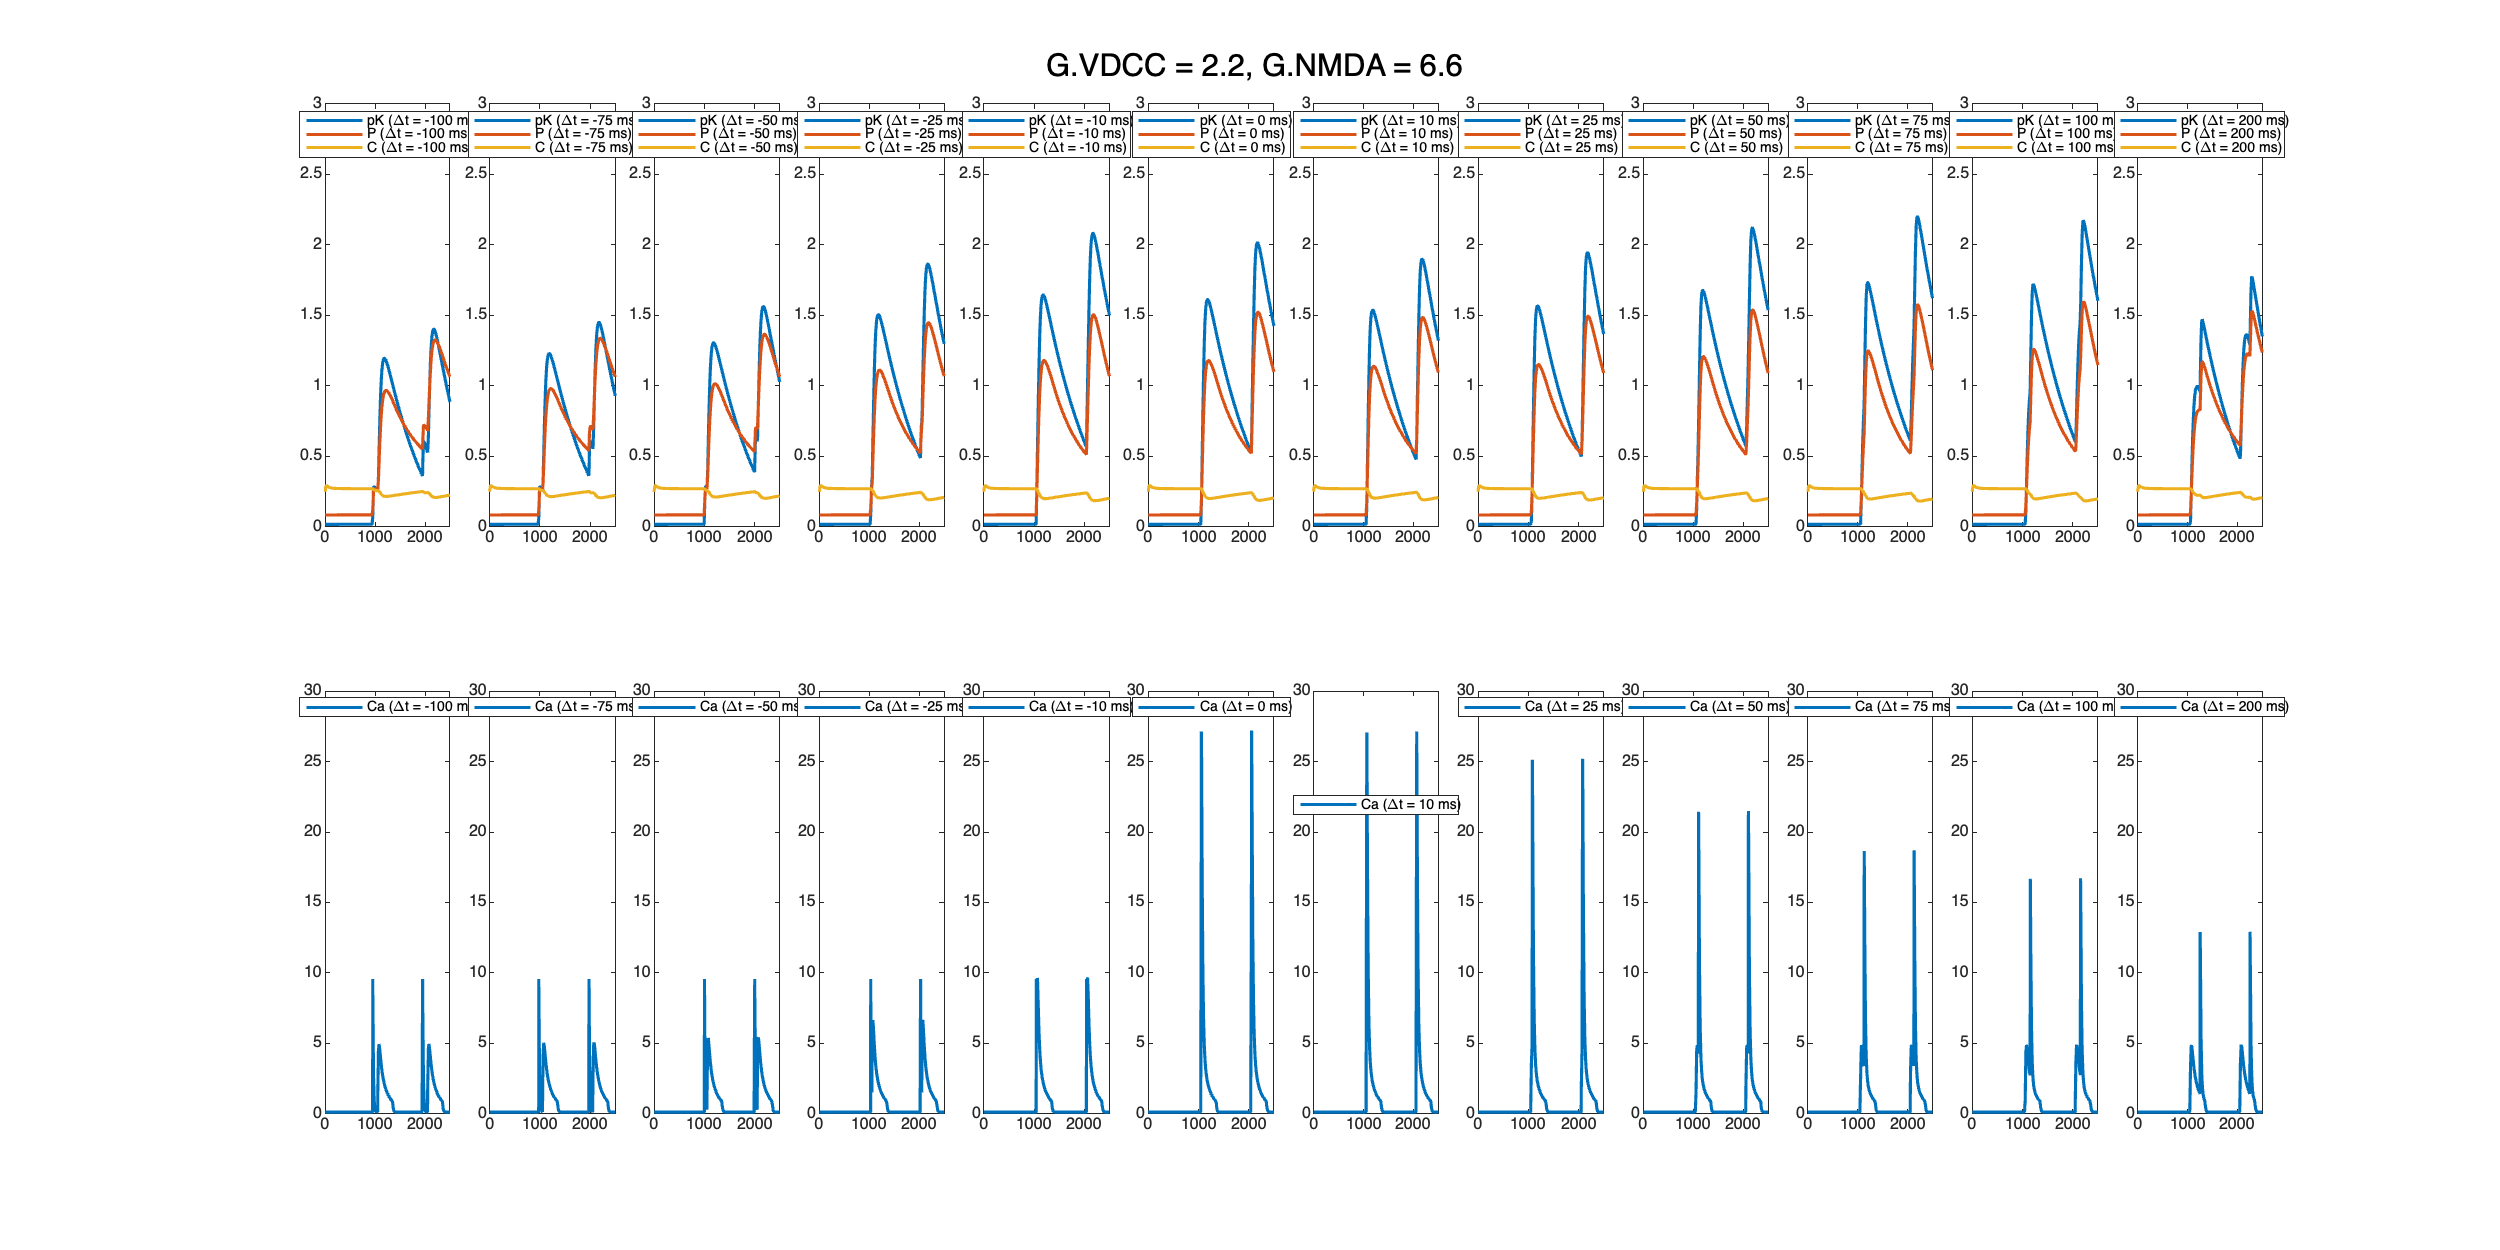
\includegraphics[width=0.8\textwidth]{a=0.1_G_VDCC=2.20_G_NMDA=6.60.png} % Change 'a=0.1.png' to your file name
    \captionof{figure}{ \( a = 0.1 \)}
    \label{fig:a0.1}
\end{minipage}

\vspace{0.5cm} % Space between plots

% Second plot
\begin{minipage}{\textwidth} % Full width for the second plot
    \centering
    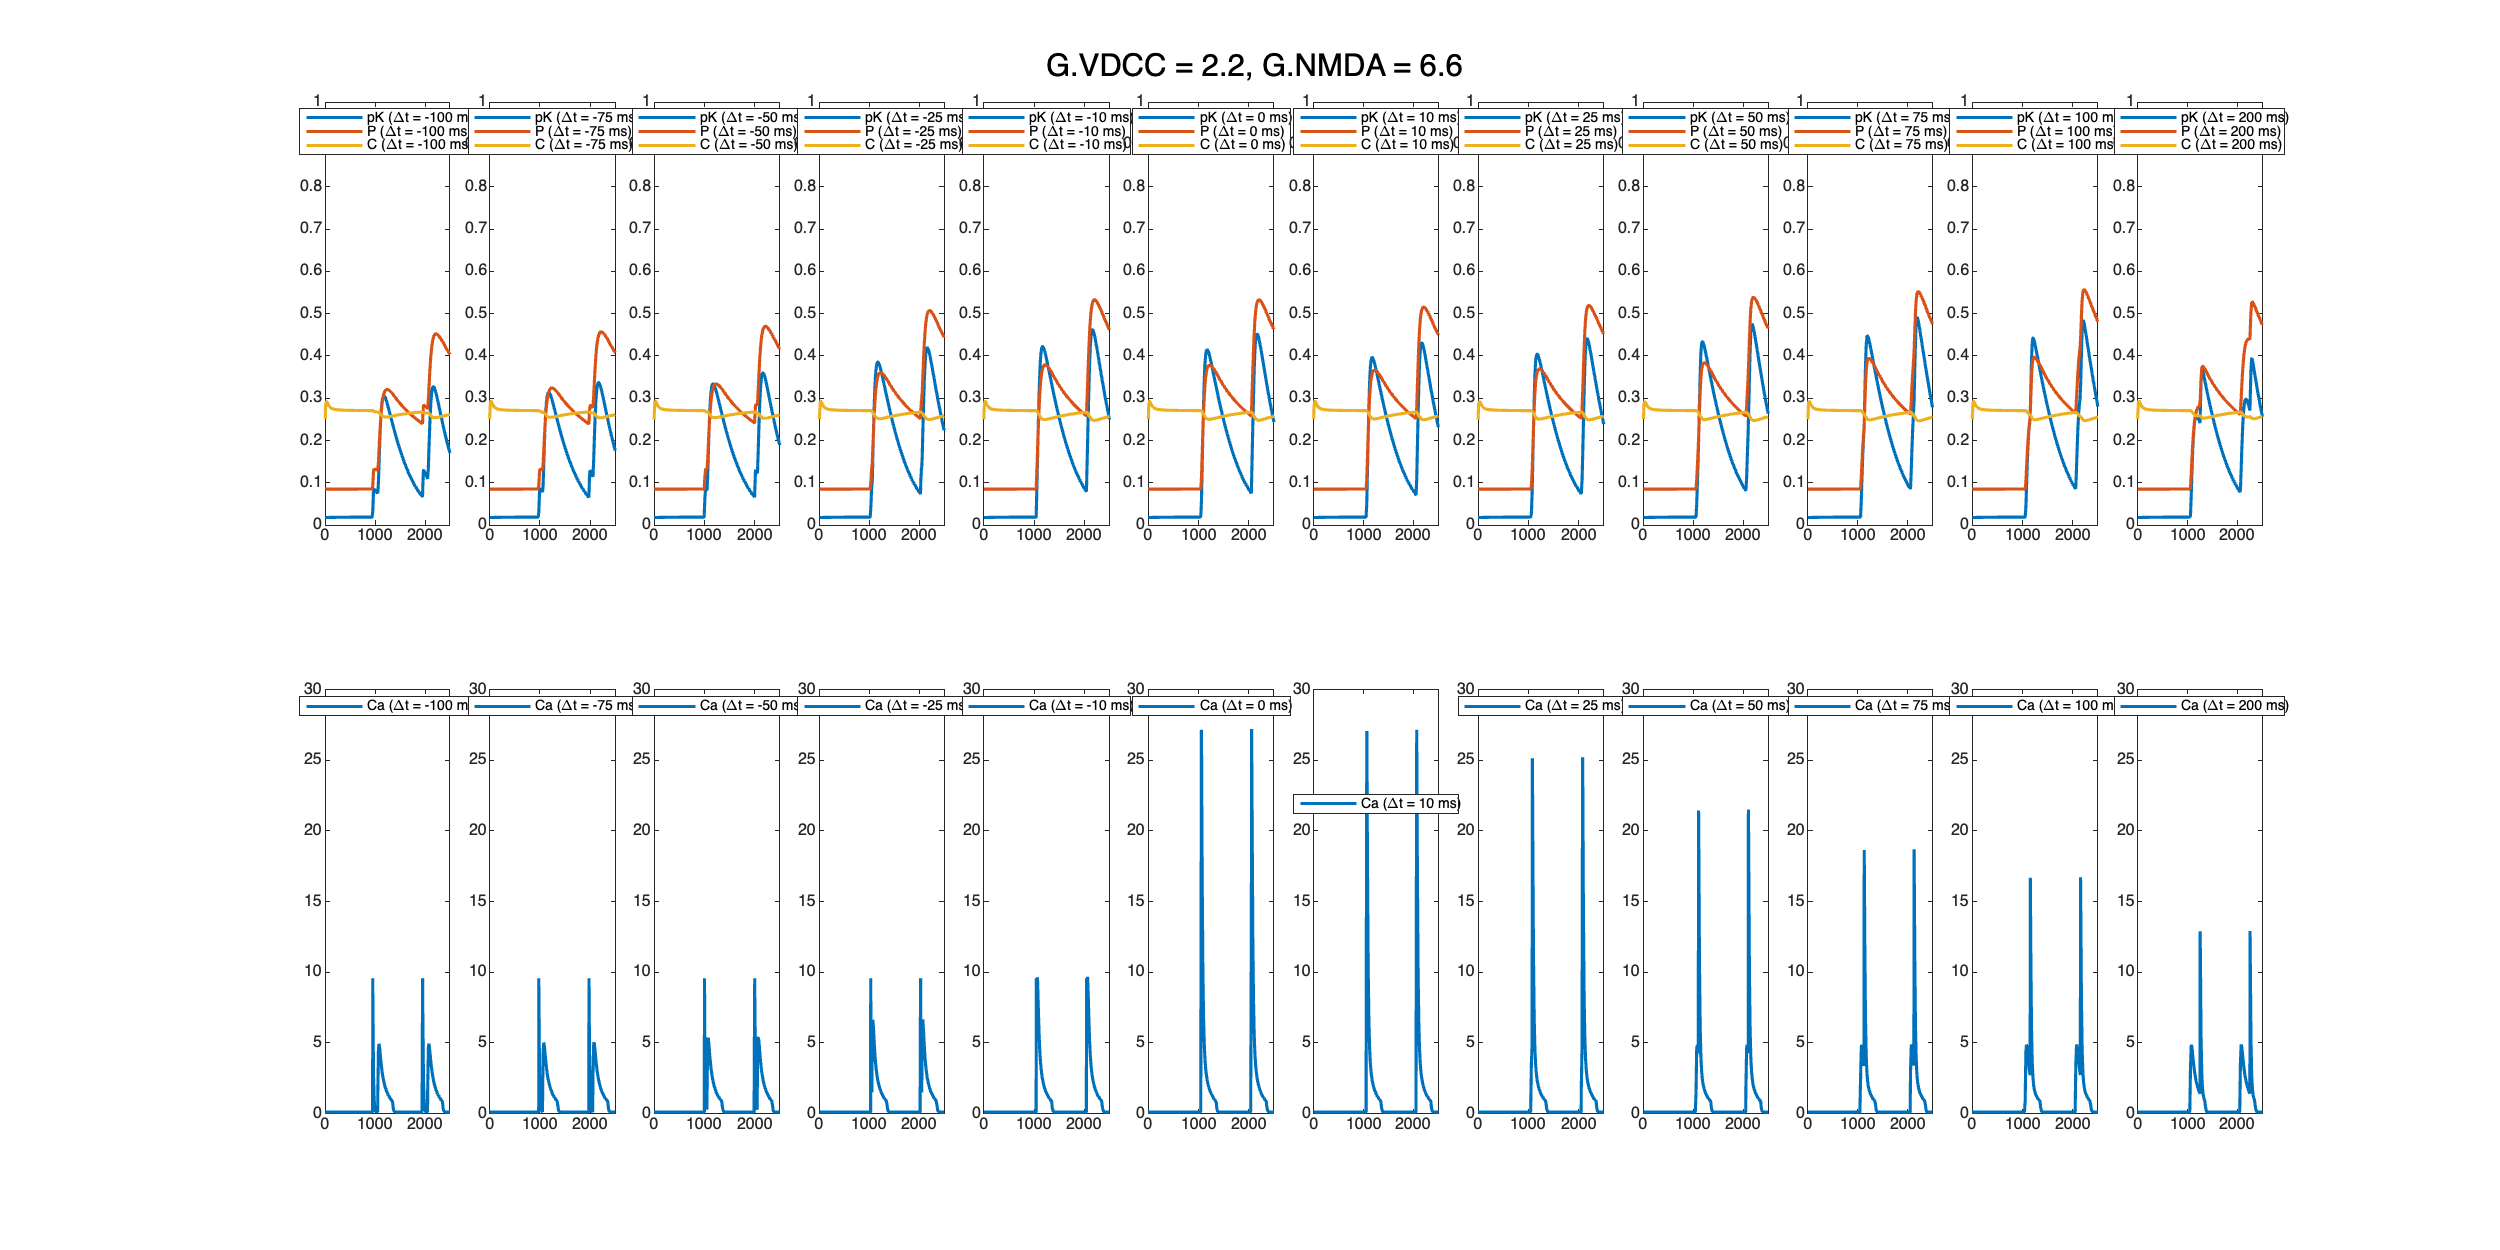
\includegraphics[width=0.8\textwidth]{a=0.25_G_VDCC=2.20_G_NMDA=6.60.png} % Change 'a=0.25.png' to your file name
    \captionof{figure}{ \( a = 0.025 \)}
    \label{fig:a0.25}
\end{minipage}

\vspace{0.5cm} % Space between plots
In the short run, we can also compare that with the same calcium profile, the system is more sensible when a is small. This can also be illustrated in the final state plot.\\
\begin{minipage}{\textwidth} % Full width for the second plot
    \centering
    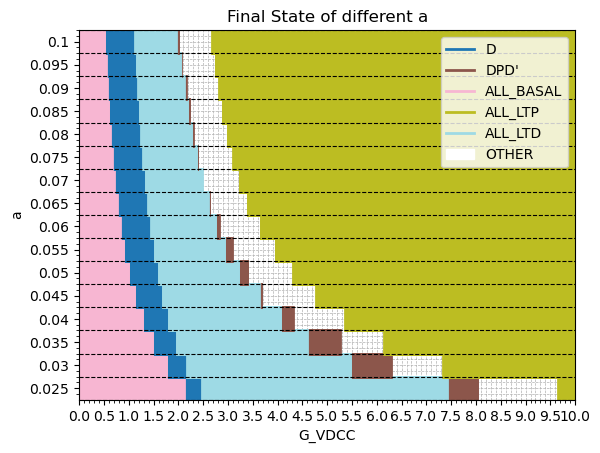
\includegraphics[width=0.45\textwidth]{a_final_state.png} % Change 'a=0.25.png' to your file name
    \captionof{figure}{final state plot}
    \label{fig:a0.25}
\end{minipage}
Here is the long run plot for $a=0.025$ for $G_{VDCC}=2.2$\\
\begin{minipage}{\textwidth} % Full width for the second plot
    \centering
    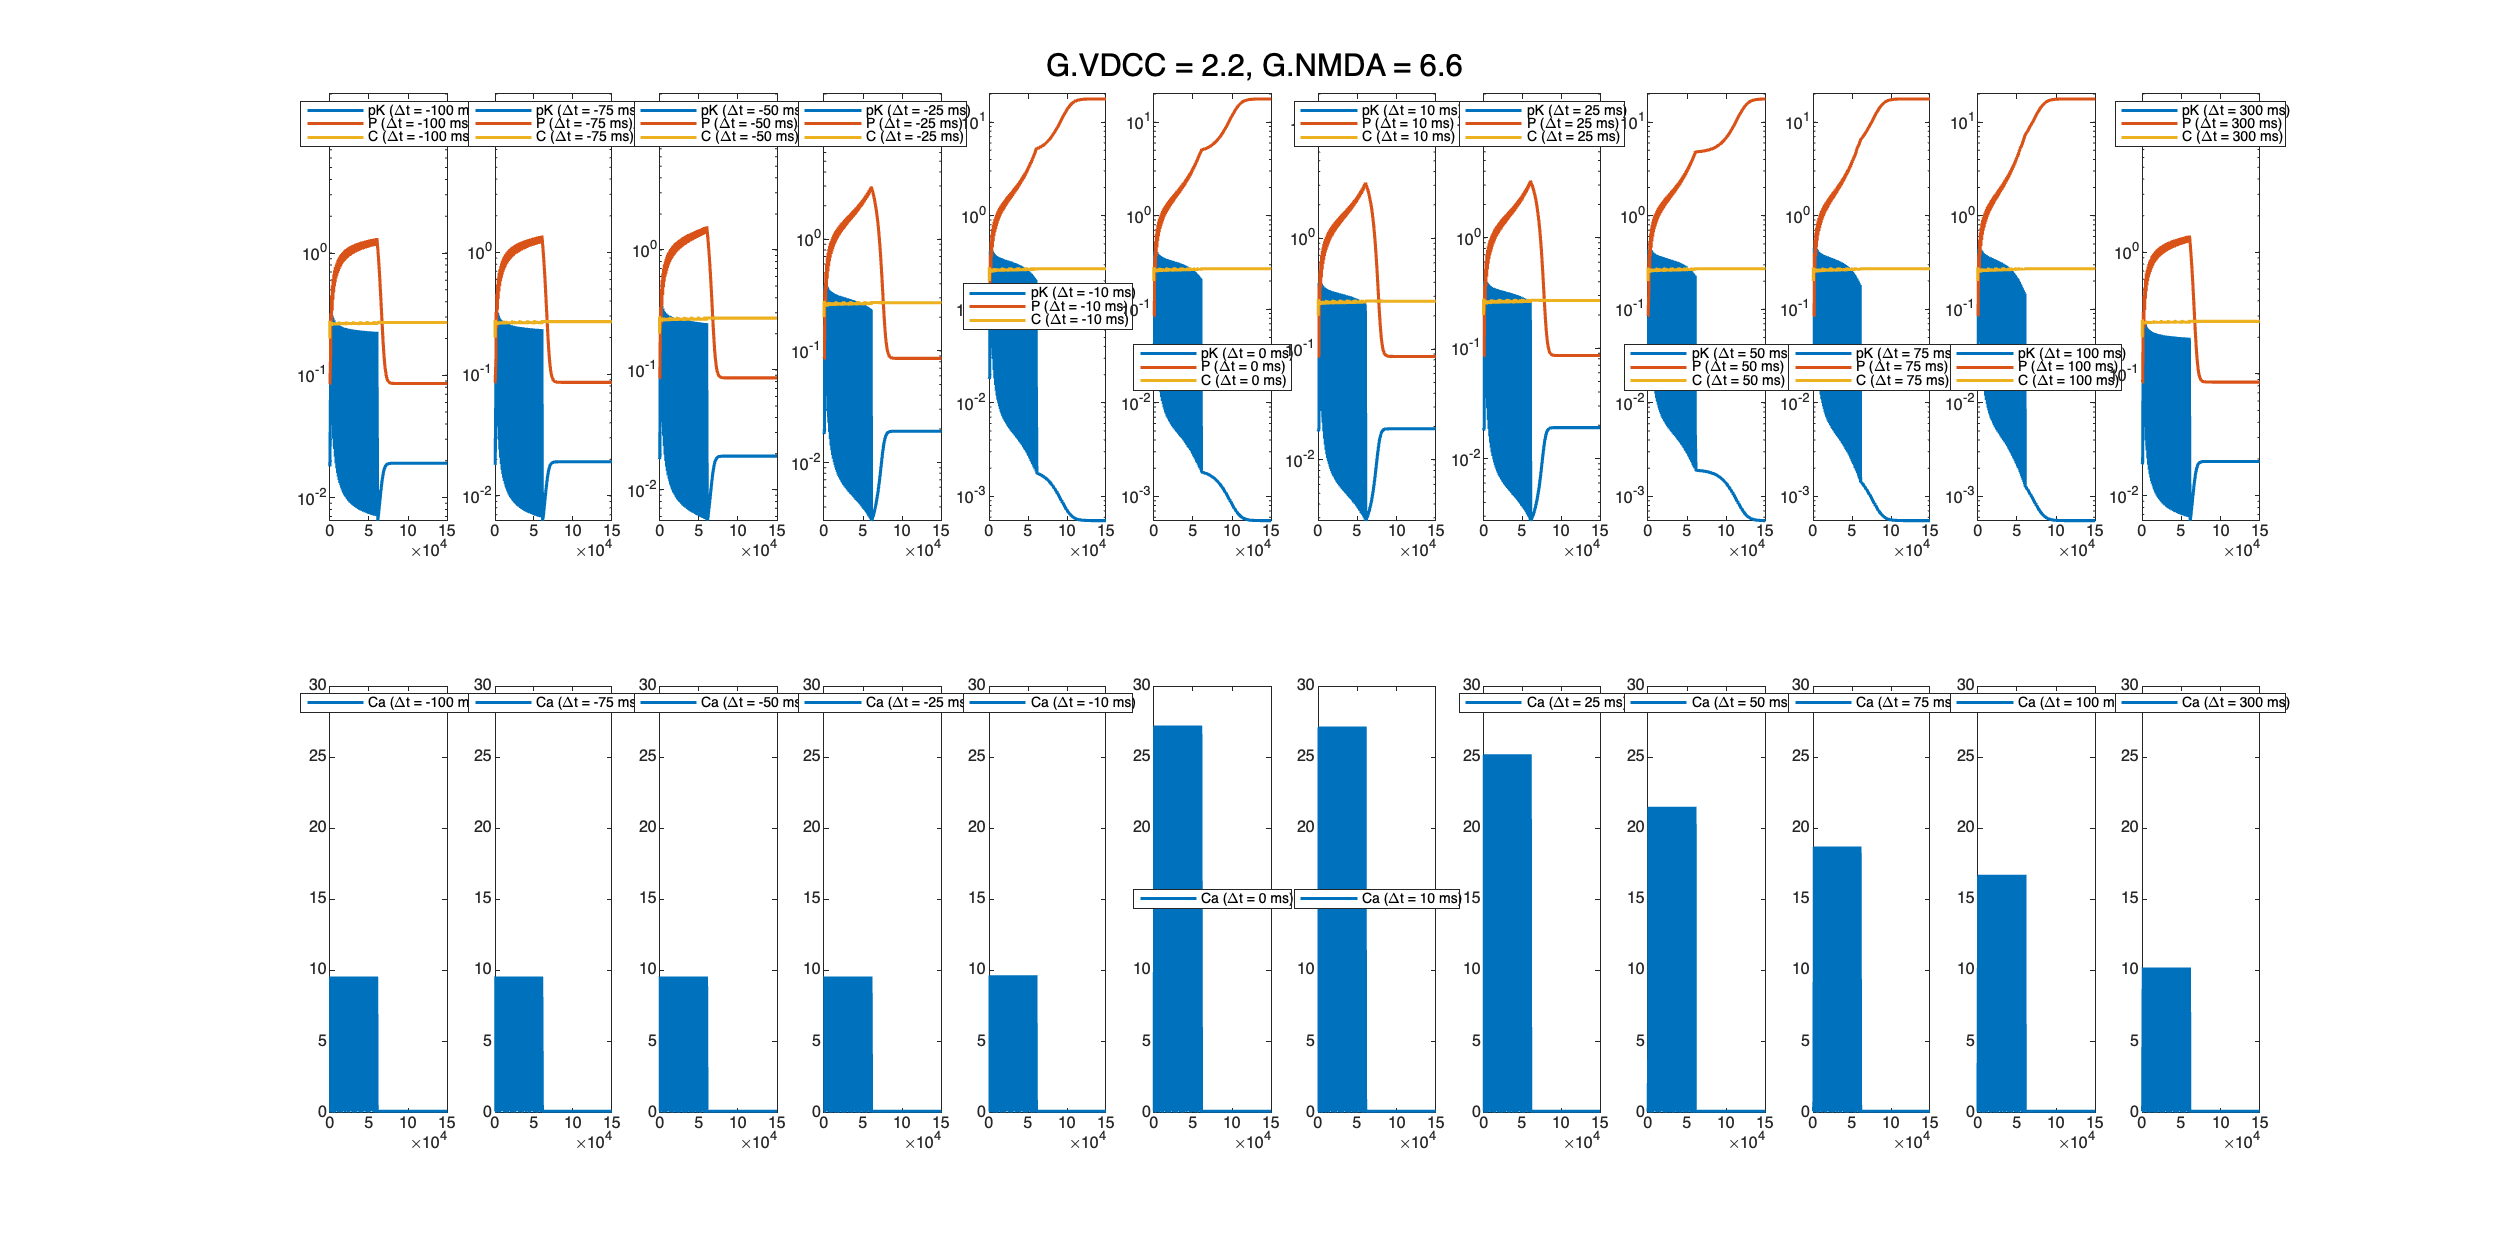
\includegraphics[width=0.8\textwidth]{a=0.025_long run G_VDCC=2.20_G_NMDA=6.60.png} % Change 'a=0.25.png' to your file name
    \captionof{figure}{ \( a = 0.025 \)}
    \label{fig:a0.25}
\end{minipage}
 When we examine the short run plot, we find that pK(blue line) decreases more than P(red line) even when pK increases more. How do we control the decay rate to make the biochemical system more balanced? Here we introduce the parameter of "km12".

\subsection{km12}
Km12 originally is equal to 1. Now we decrease Km12, and the result is as following:\\
\begin{minipage}{\textwidth} % Full width for the second plot
    \centering
    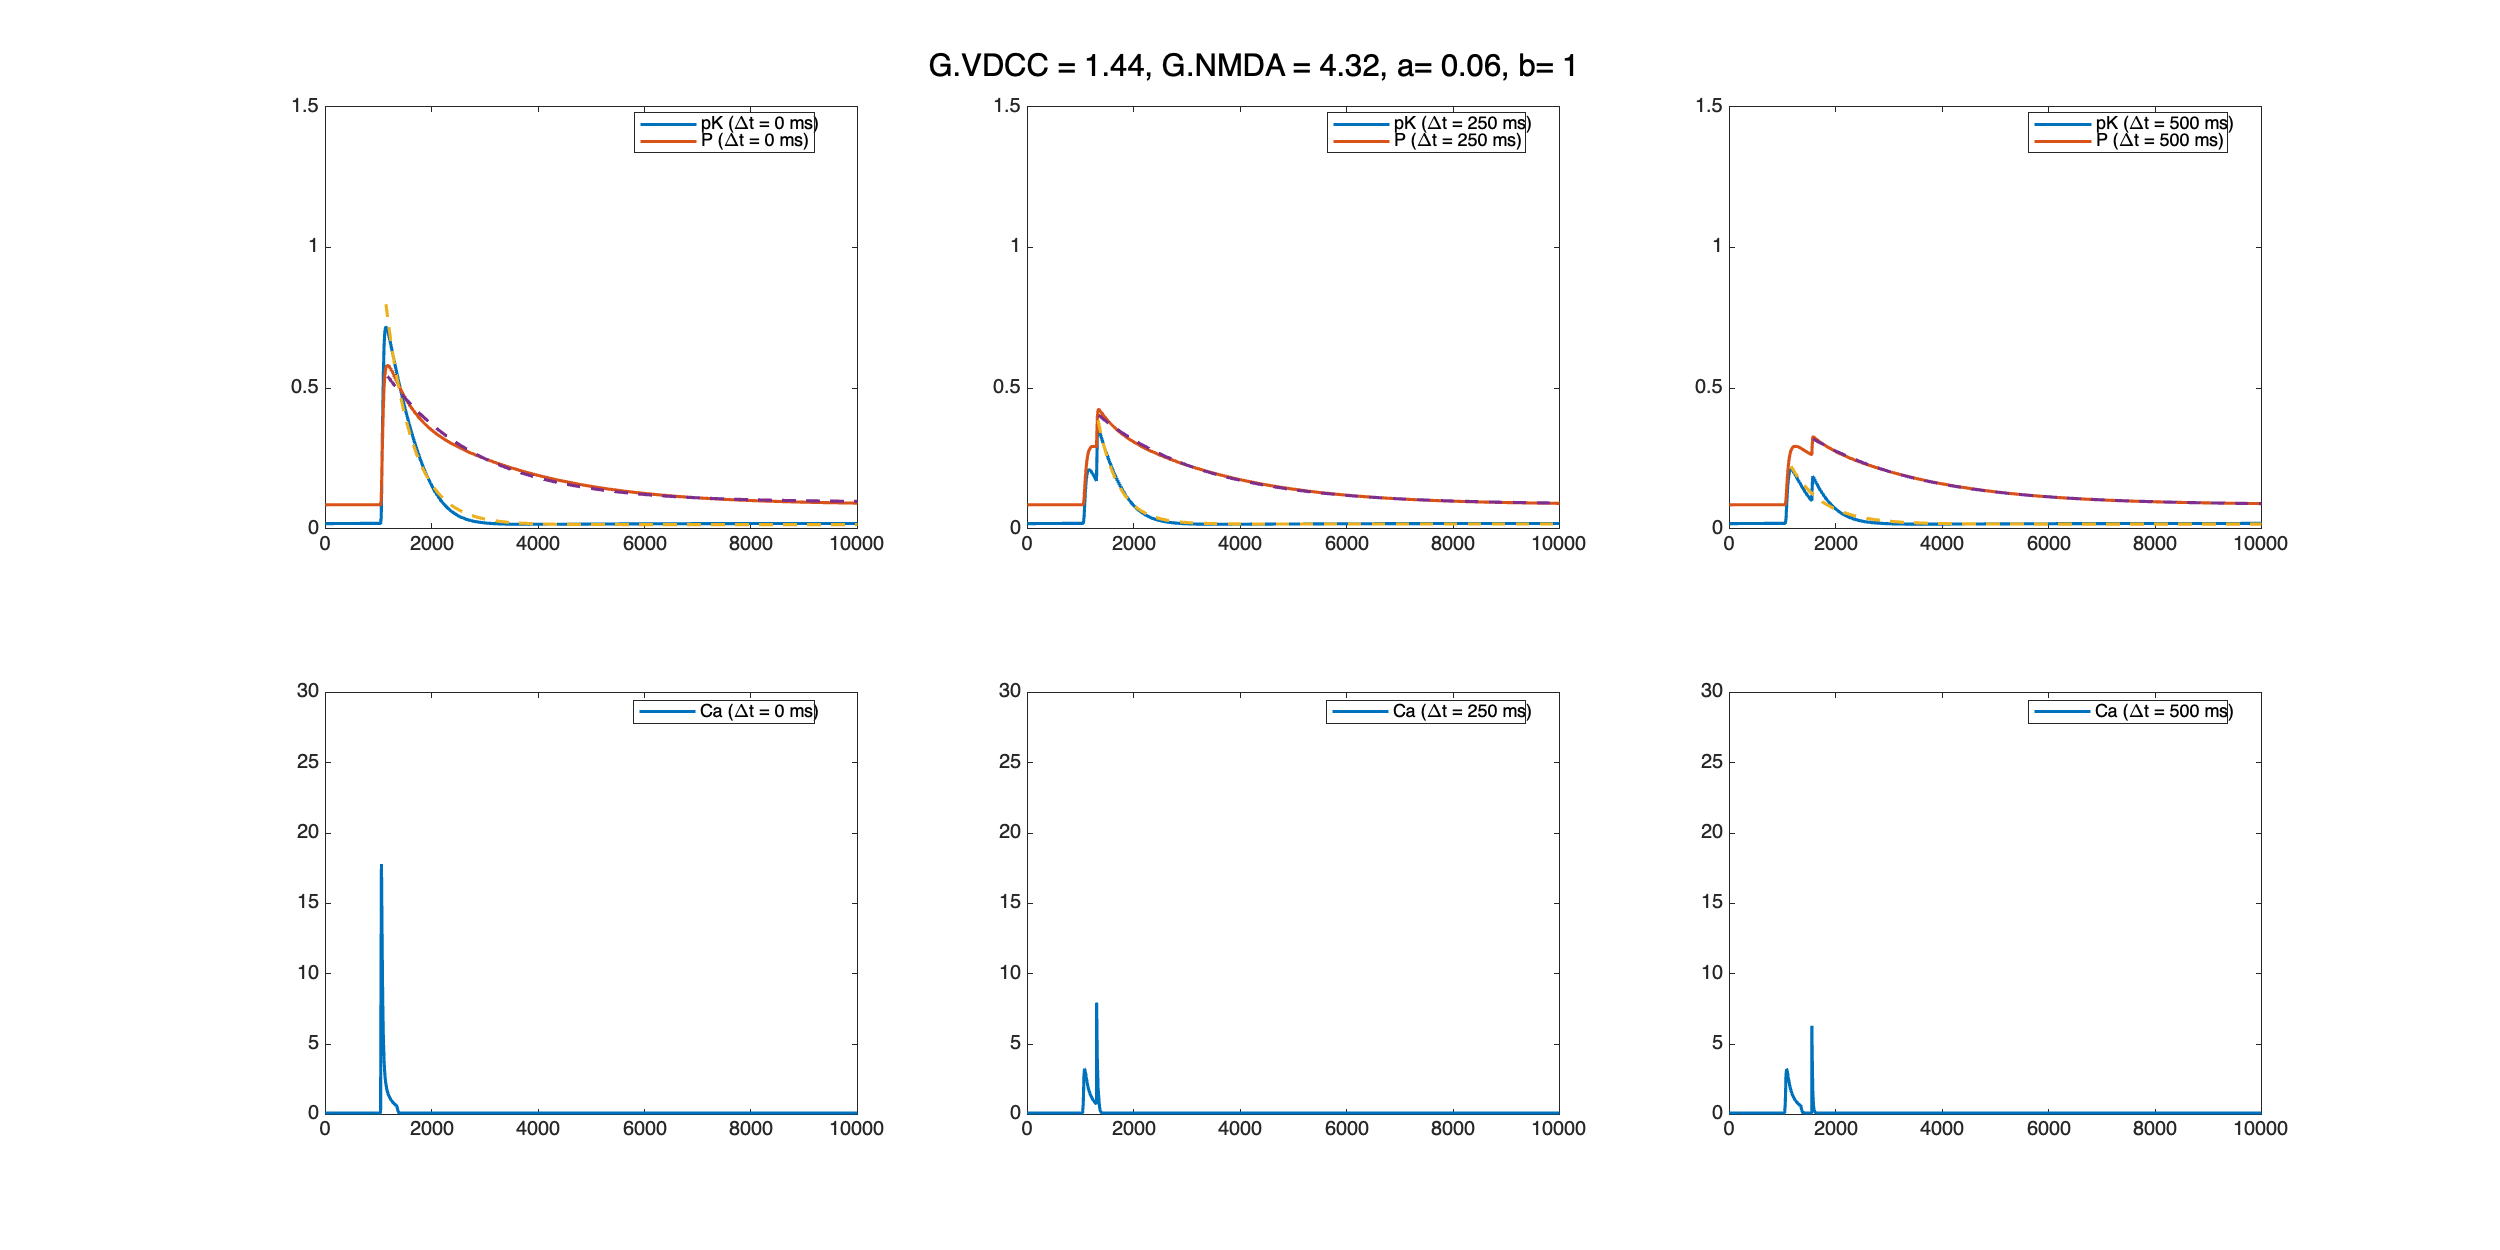
\includegraphics[width=0.8\textwidth]{G_VDCC=1.44_G_NMDA=4.32_a=0.060 b=1.00.png} % Change 'a=0.25.png' to your file name
    \captionof{figure}{ \( b=1.00 \)}
    \label{fig:a0.25}
\end{minipage}
\begin{minipage}{\textwidth} % Full width for the second plot
    \centering
    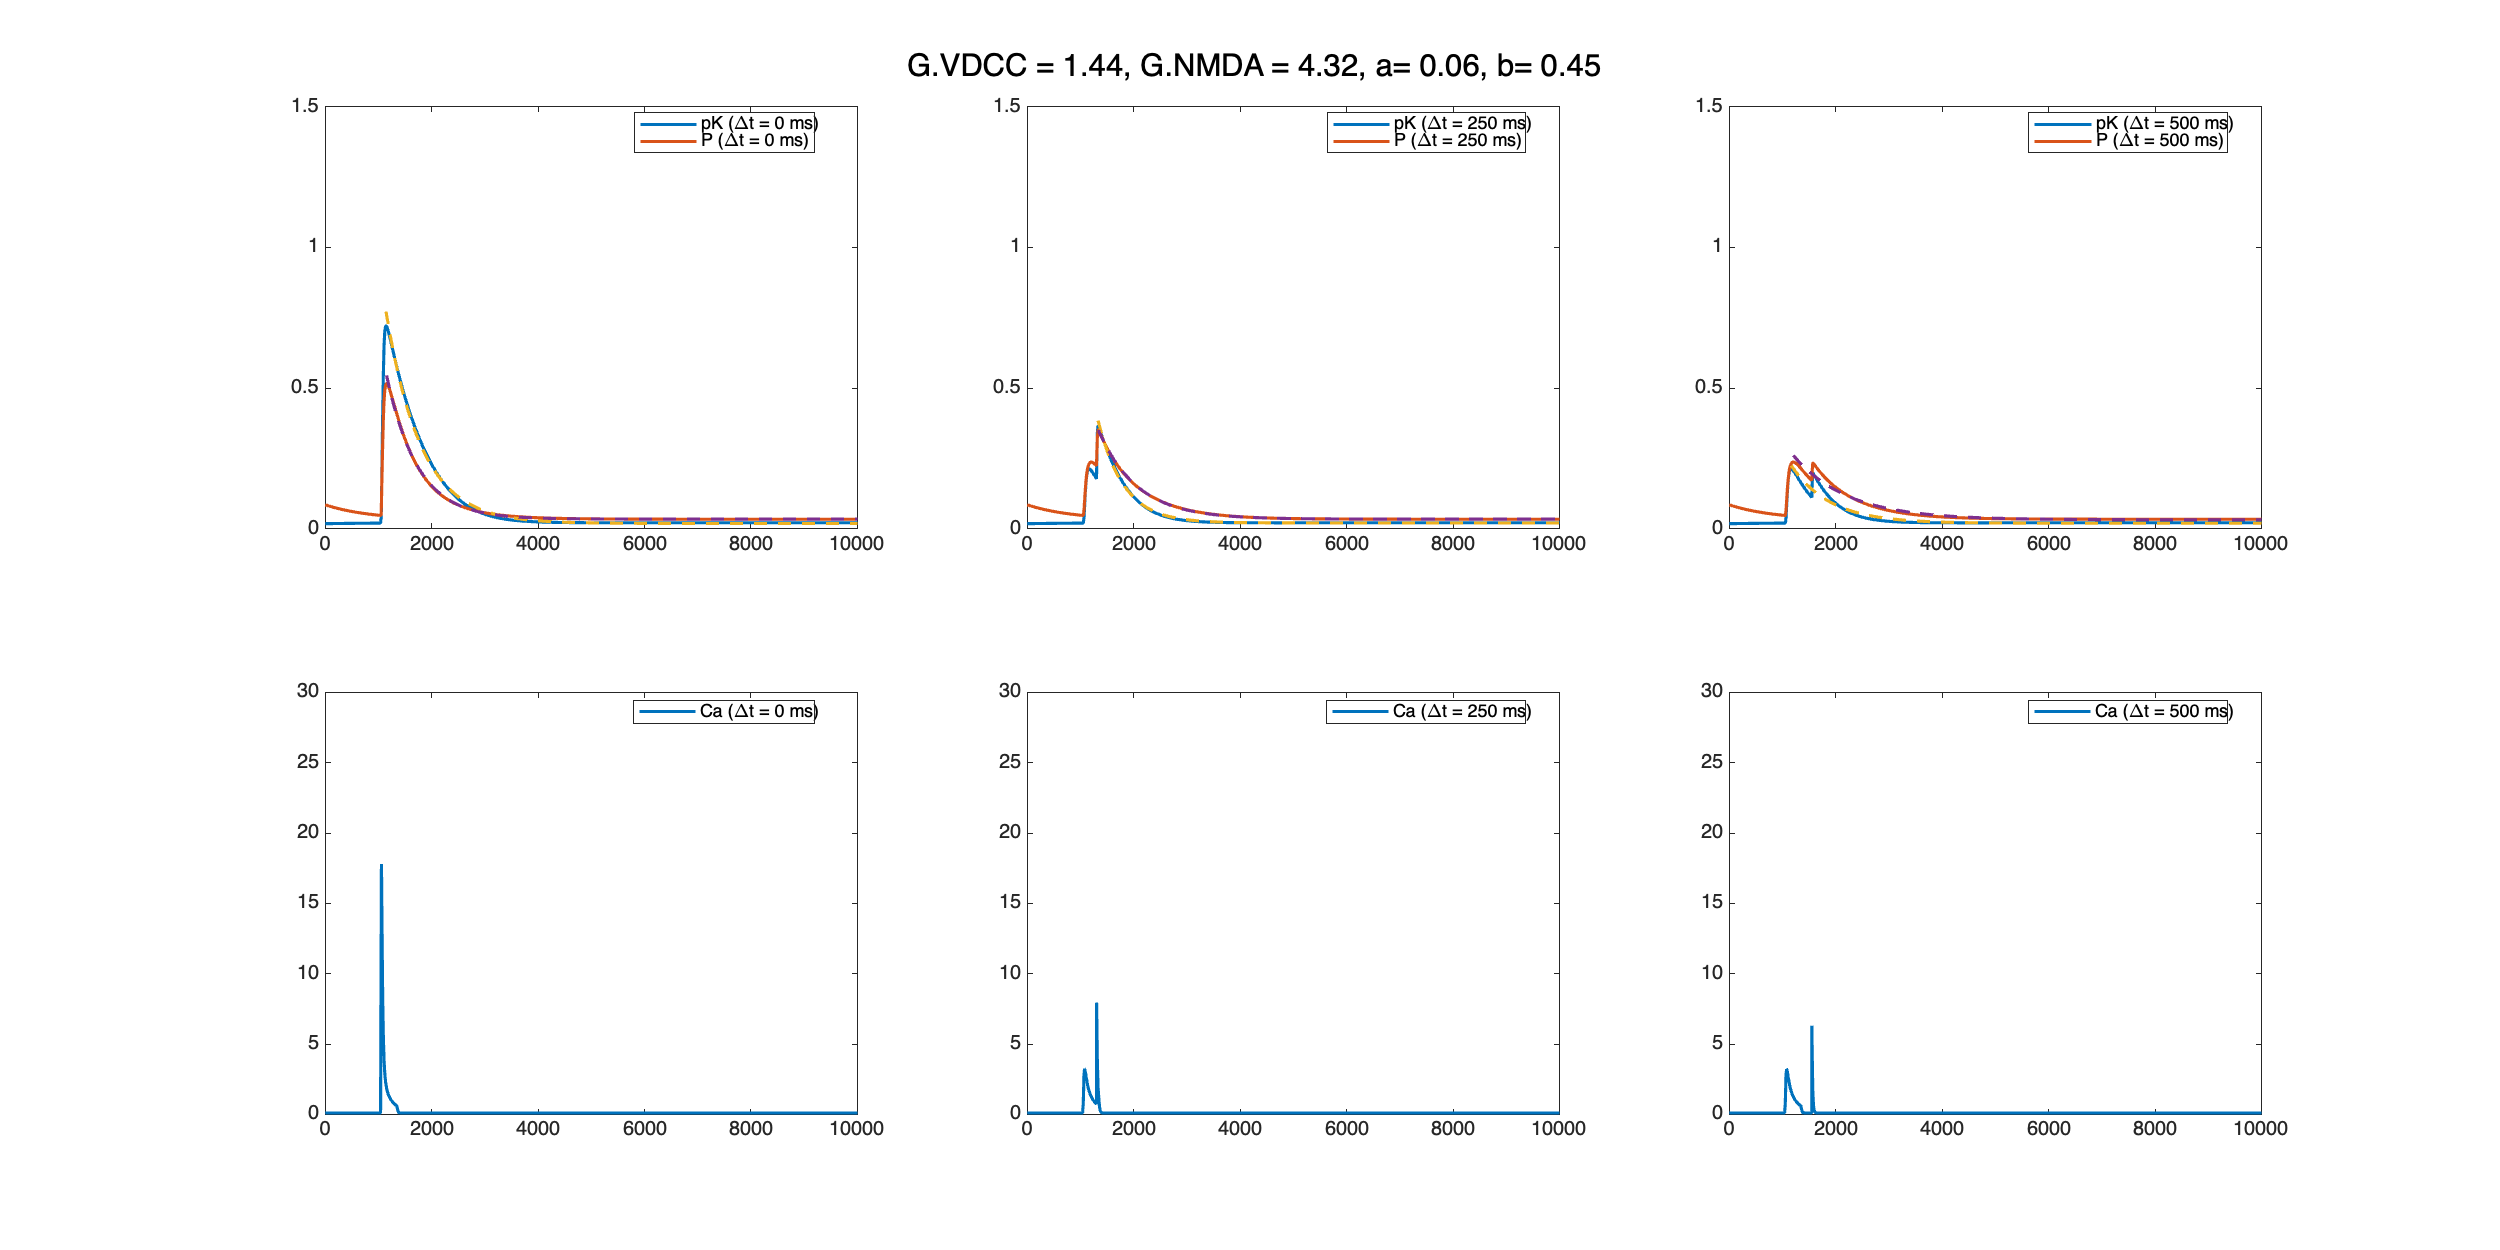
\includegraphics[width=0.8\textwidth]{G_VDCC=1.44_G_NMDA=4.32_a=0.060 b=0.45.png} % Change 'a=0.25.png' to your file name
    \captionof{figure}{ \( b=0.45 \)}
    \label{fig:a0.25}
\end{minipage}
\begin{minipage}{\textwidth} % Full width for the second plot
    \centering
    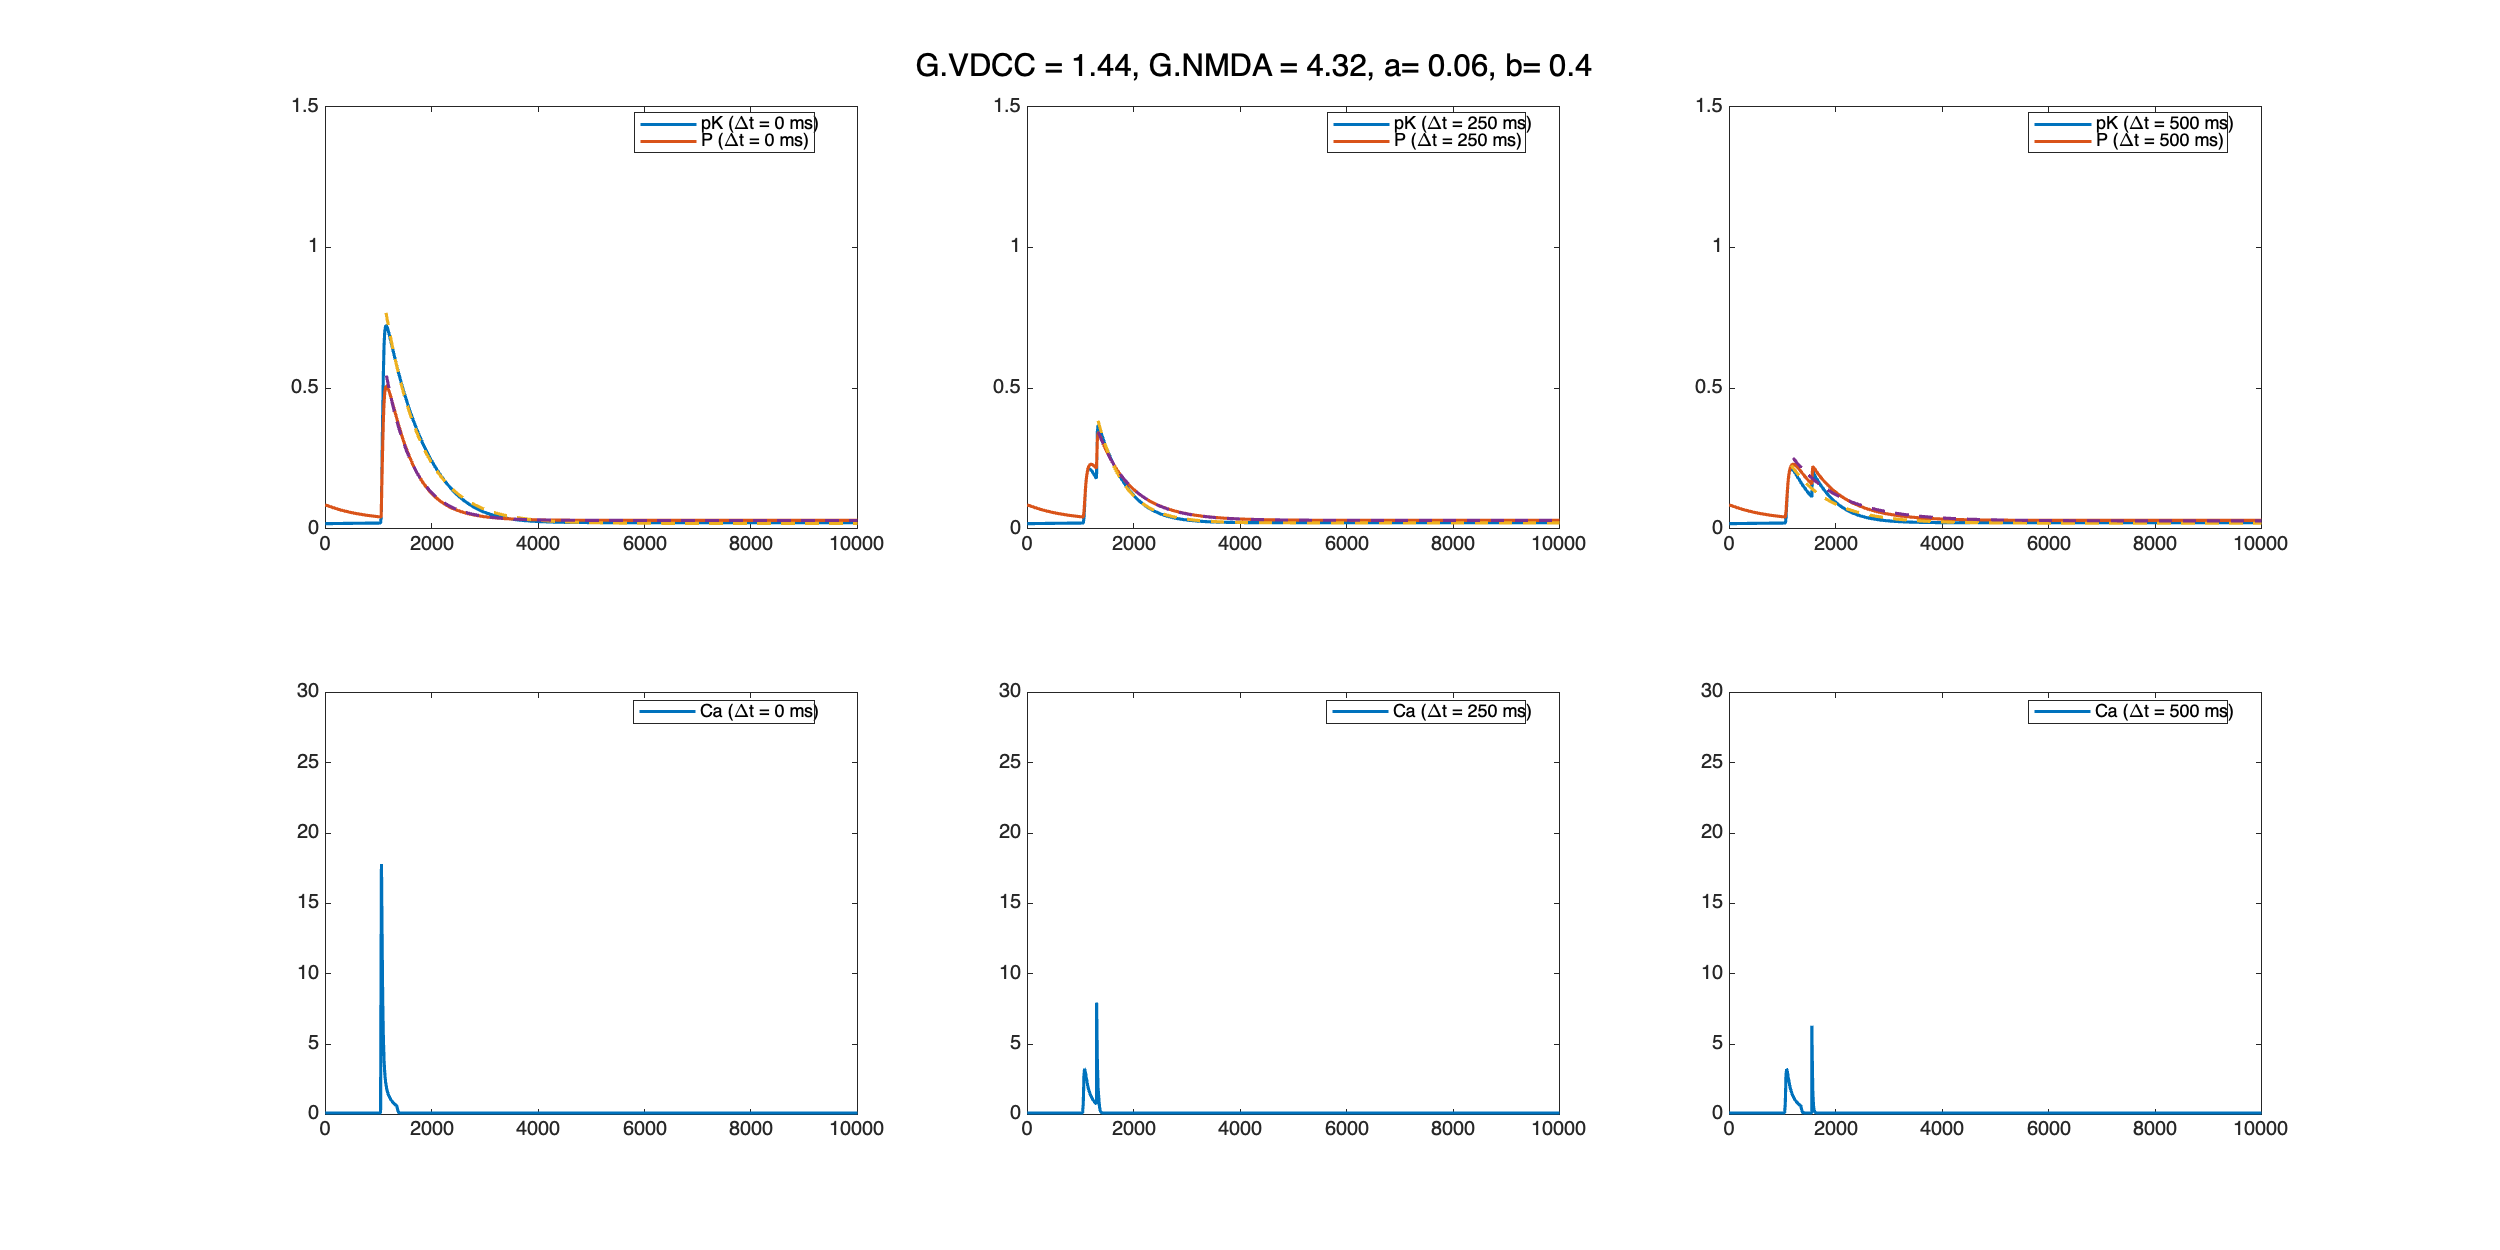
\includegraphics[width=0.8\textwidth]{G_VDCC=1.44_G_NMDA=4.32_a=0.060 b=0.40.png} % Change 'a=0.25.png' to your file name
    \captionof{figure}{ \( b=0.40 \)}
    \label{fig:a0.25}
\end{minipage}
\begin{minipage}{\textwidth} % Full width for the second plot
    \centering
    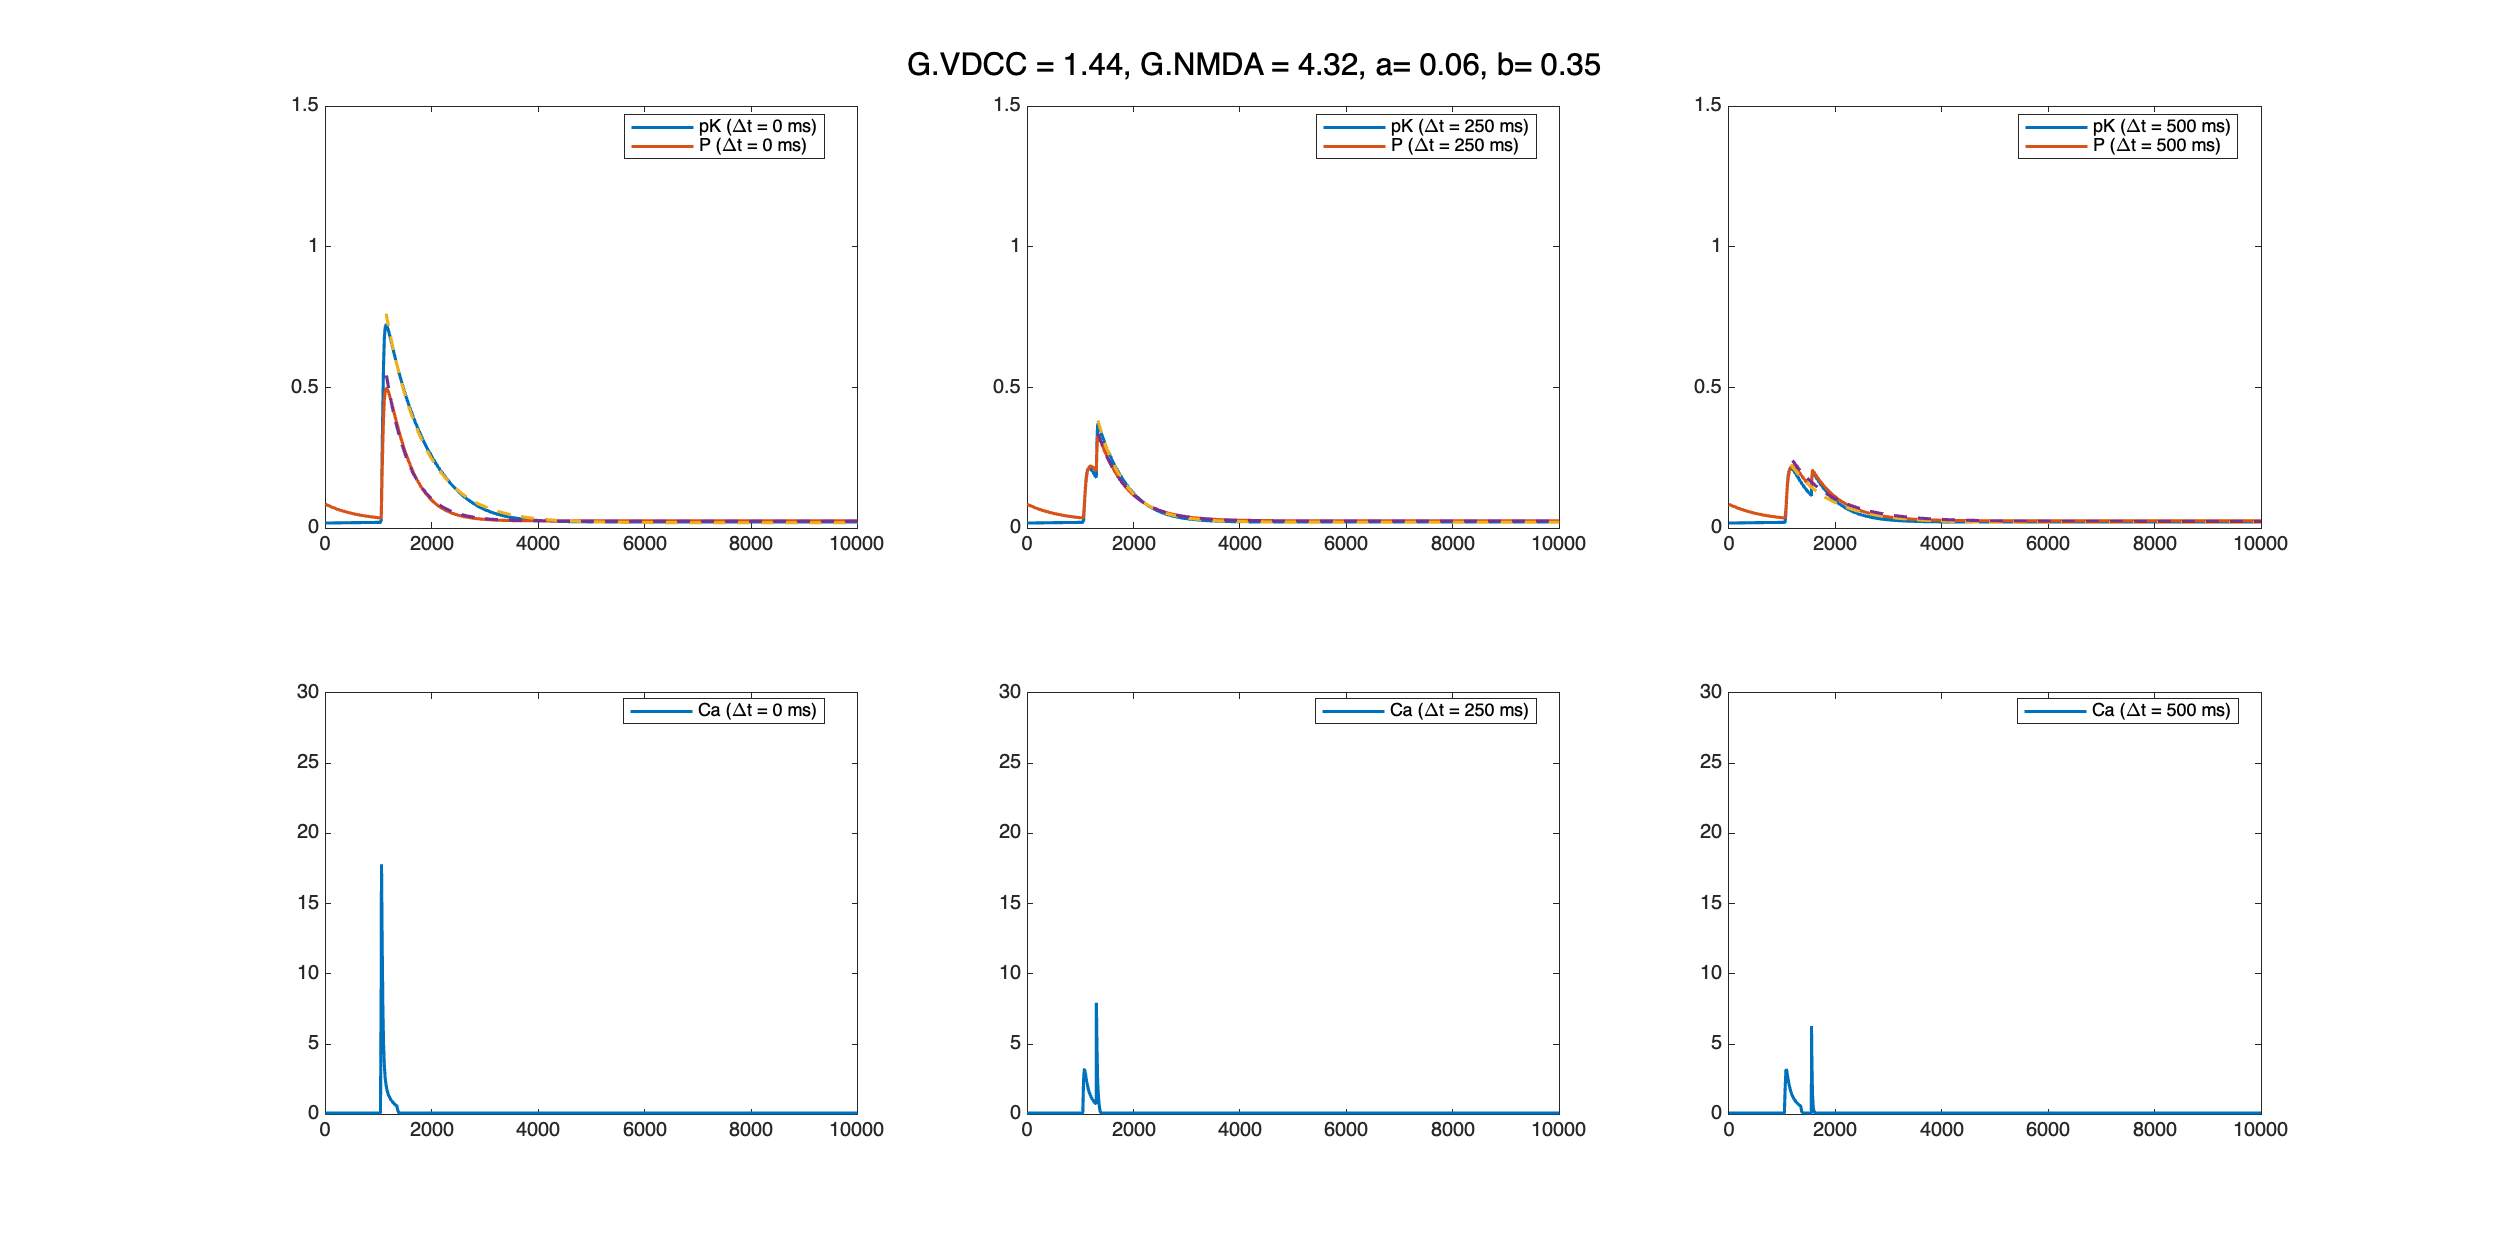
\includegraphics[width=0.8\textwidth]{G_VDCC=1.44_G_NMDA=4.32_a=0.060 b=0.35.png} % Change 'a=0.25.png' to your file name
    \captionof{figure}{ \( b=0.35 \)}
    \label{fig:a0.25}
\end{minipage}
If we compare this plot, as km12 decrease, P actually decrease faster.
\begin{figure}[h]
    \centering
    \begin{minipage}[b]{0.45\textwidth}
        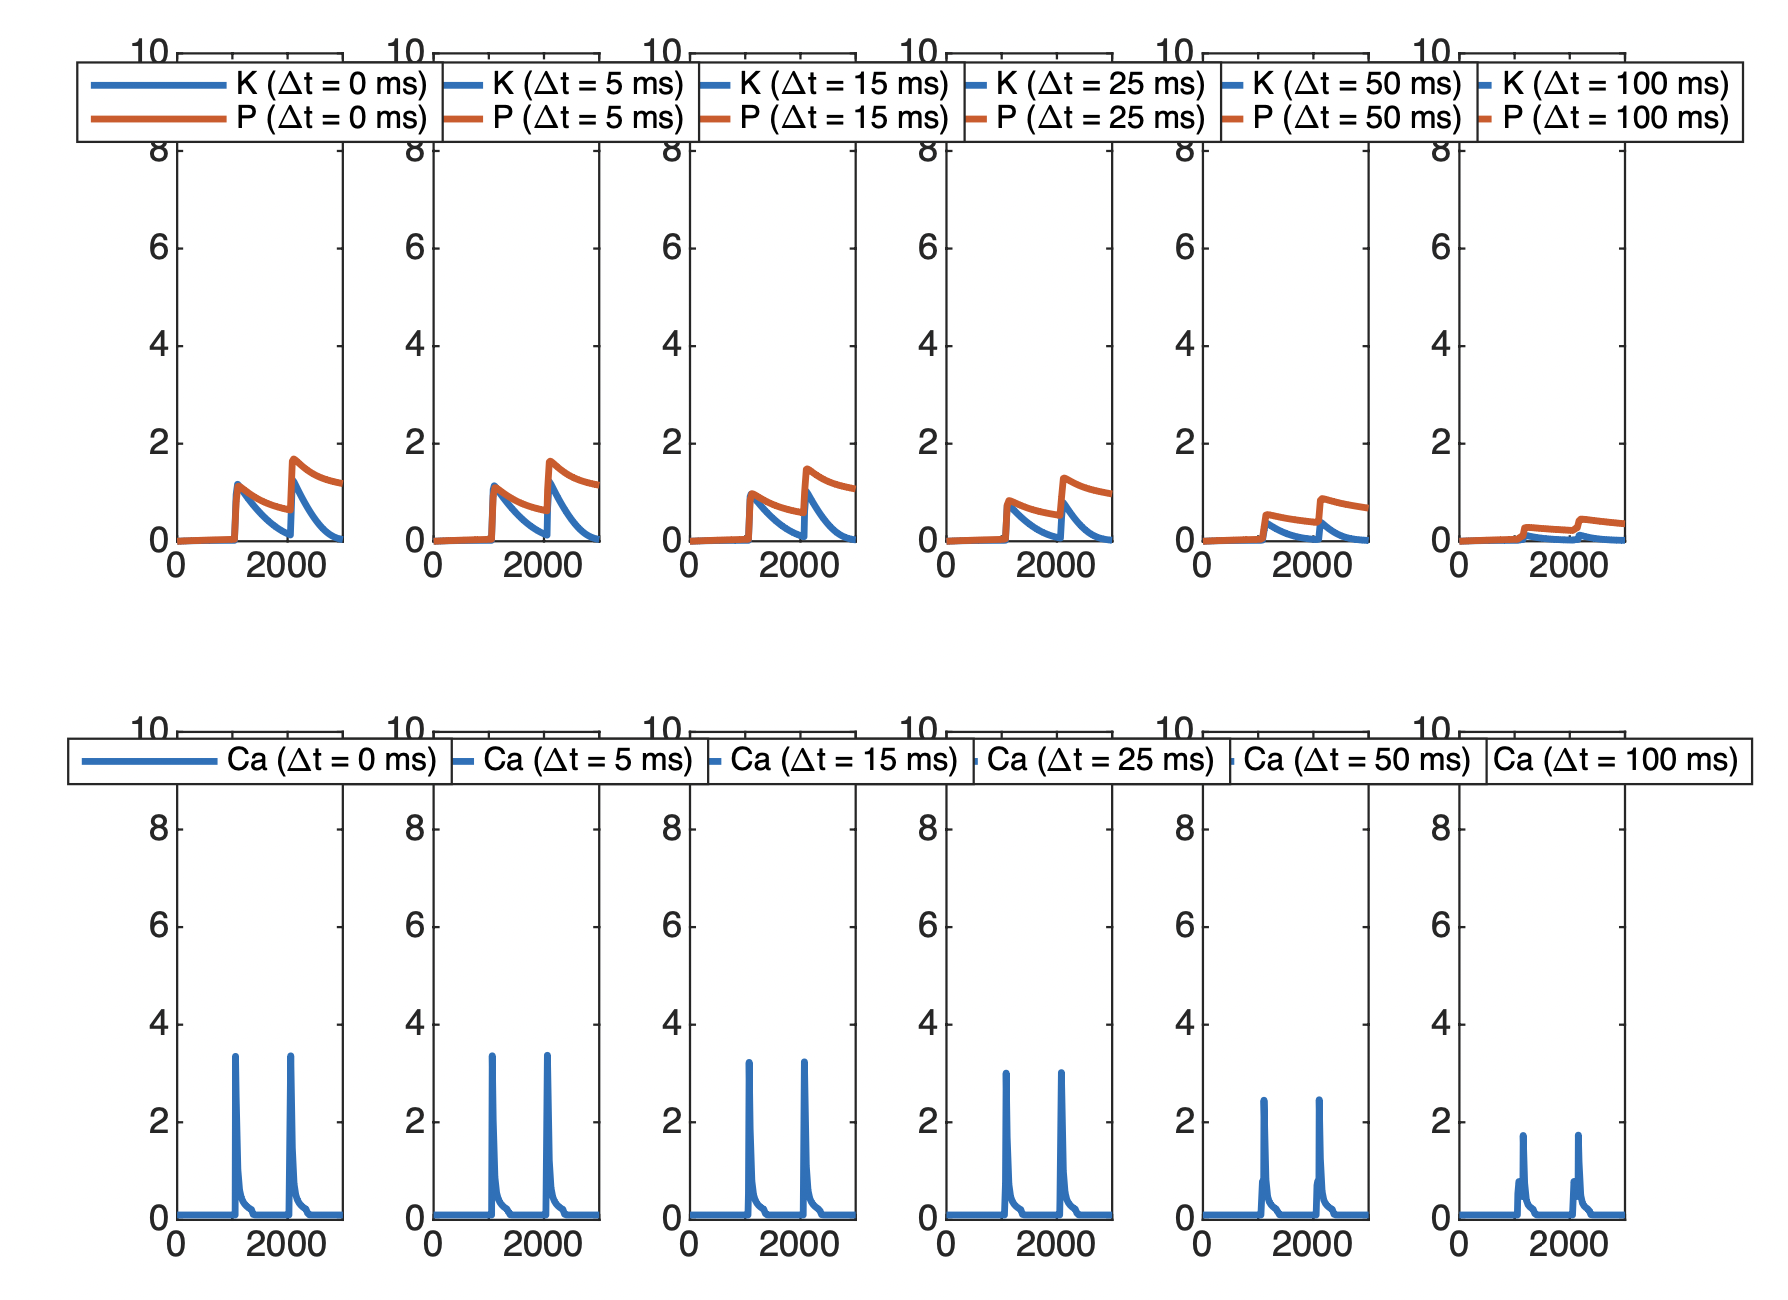
\includegraphics[width=1.1\textwidth]{0.1.png}
        \caption{$G_{NMDA}=0.2,G_{VDCC}=1.3$}
        \label{fig:image1}
    \end{minipage}
    \hfill % or \hspace*{\fill} to have space between the two figures
    \begin{minipage}[b]{0.45\textwidth}
        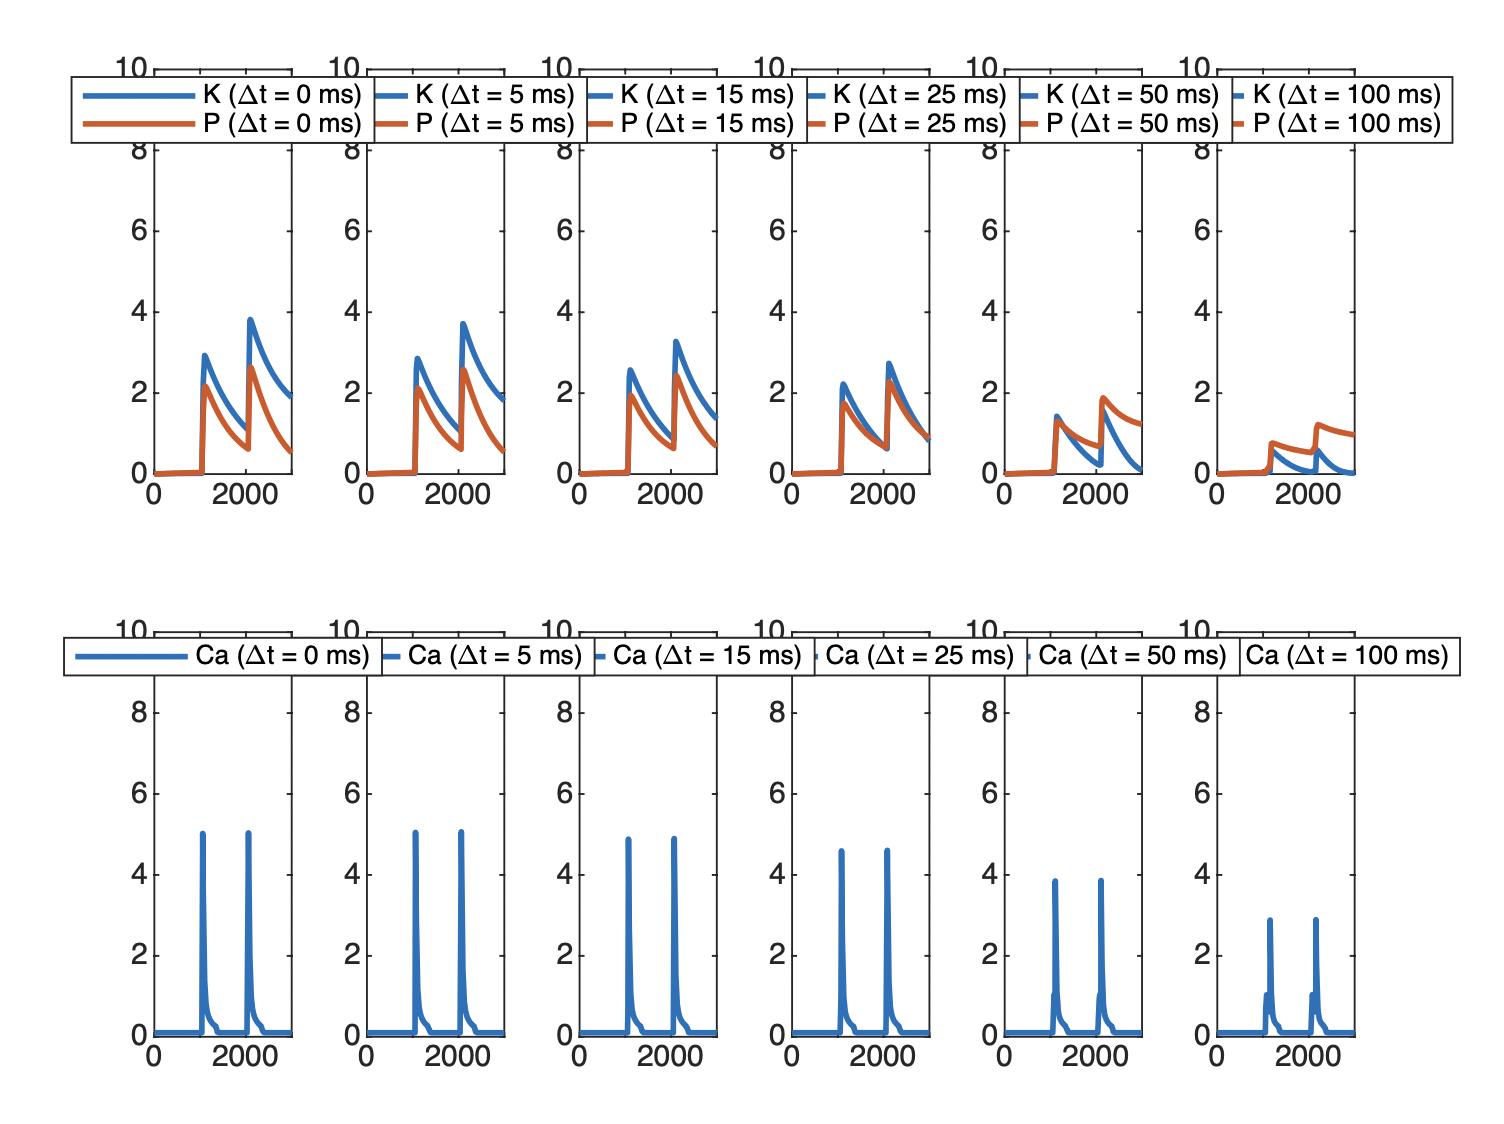
\includegraphics[width=\textwidth]{0.3.png}
        \caption{$G_{NMDA}=0.1,G_{VDCC}=0.95$}
        \label{fig:image2}
    \end{minipage}
\end{figure}\\
If we check its phase diagram for different km12 value, the result follows:
\begin{figure}[h]
    \centering
    \begin{minipage}[b]{0.45\textwidth}
        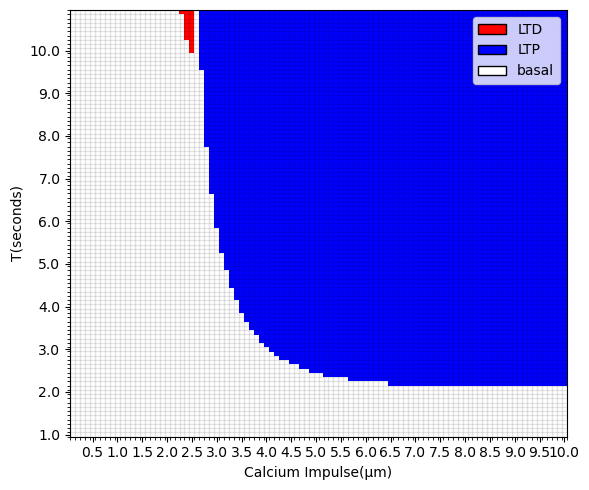
\includegraphics[width=1.1\textwidth]{a=0.04 km12=0.4.png}
        \caption{$a=0.04, km12=0.4$}
        \label{fig:image1}
    \end{minipage}
    \hfill % or \hspace*{\fill} to have space between the two figures
    \begin{minipage}[b]{0.45\textwidth}
        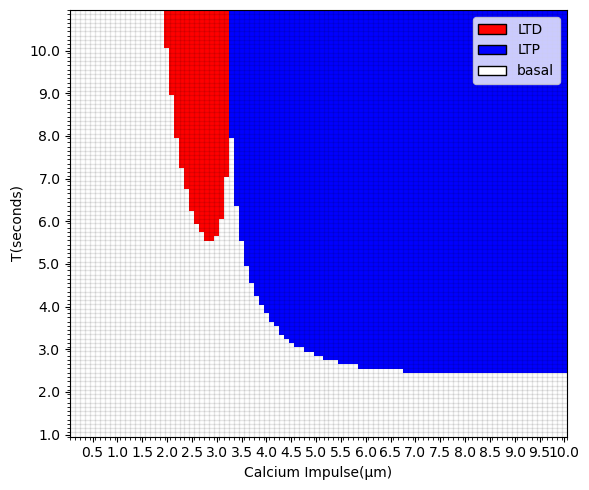
\includegraphics[width=\textwidth]{a=0.04 km12=1.png}
        \caption{$a=0.04, km12=1$}
        \label{fig:image2}
    \end{minipage}
\end{figure}\\
The result from phase diagram actually tells us under the same assumption, decreasing the km12 will make the decay rate more balanced but at the cost of LTD become dominant. It can be illustrated in the following color plot.\\
\begin{minipage}{\textwidth} % Full width for the second plot
    \centering
    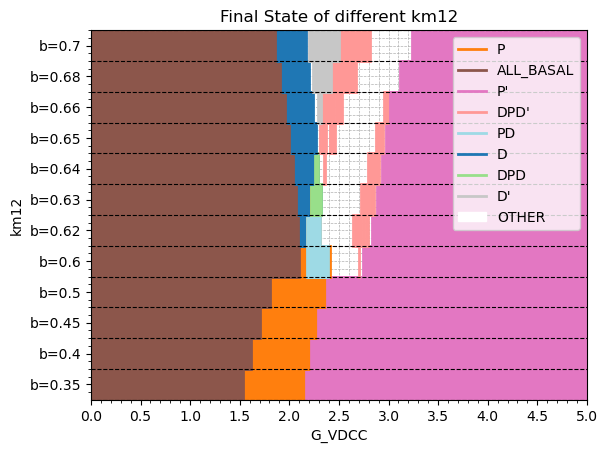
\includegraphics[width=0.8\textwidth]{fix a=0.04.png} % Change 'a=0.25.png' to your file name
    \captionof{figure}{\( a=0.04 \)}
    \label{fig:a0.25}
\end{minipage}\\
Therefore, in order to balance of LTD and LTP with decay rate being matched(low km12 value), the natural step for us is to increase a. The result if as following:
\begin{figure}[h]
    \centering
    \begin{minipage}[b]{0.45\textwidth}
        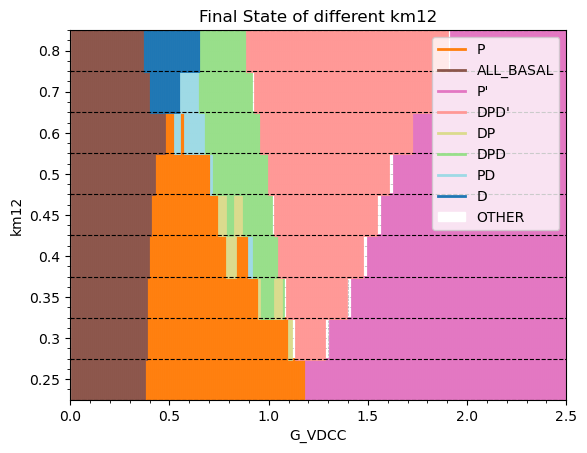
\includegraphics[width=1\textwidth]{a=0.2_final_state.png}
        \caption{$a=0.2$}
        \label{fig:image1}
    \end{minipage}
    \hfill % or \hspace*{\fill} to have space between the two figures
    \begin{minipage}[b]{0.45\textwidth}
        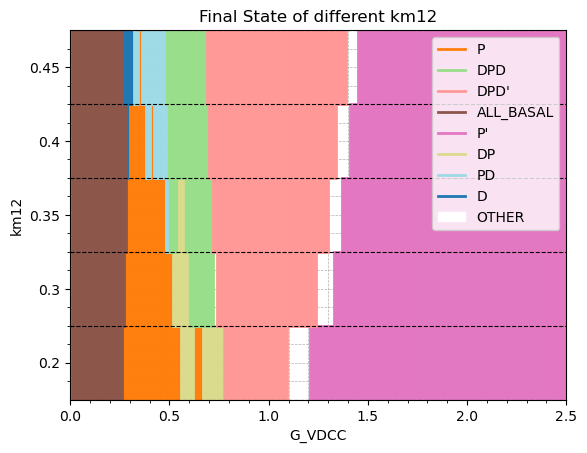
\includegraphics[width=\textwidth]{a=0.5_final_state.png}
        \caption{$a=0.5$}
        \label{fig:image2}
    \end{minipage}
\end{figure}\\
In this setting actually, we can observe some DP, but it is in the LTP preferred region. In real case, we are expecting it is in the LTD preferred region. Here is the short run/long run plot for some DP. Note that short run and long run have different $\Delta t$ setting\\
\begin{minipage}{\textwidth} % Full width for the second plot
    \centering
    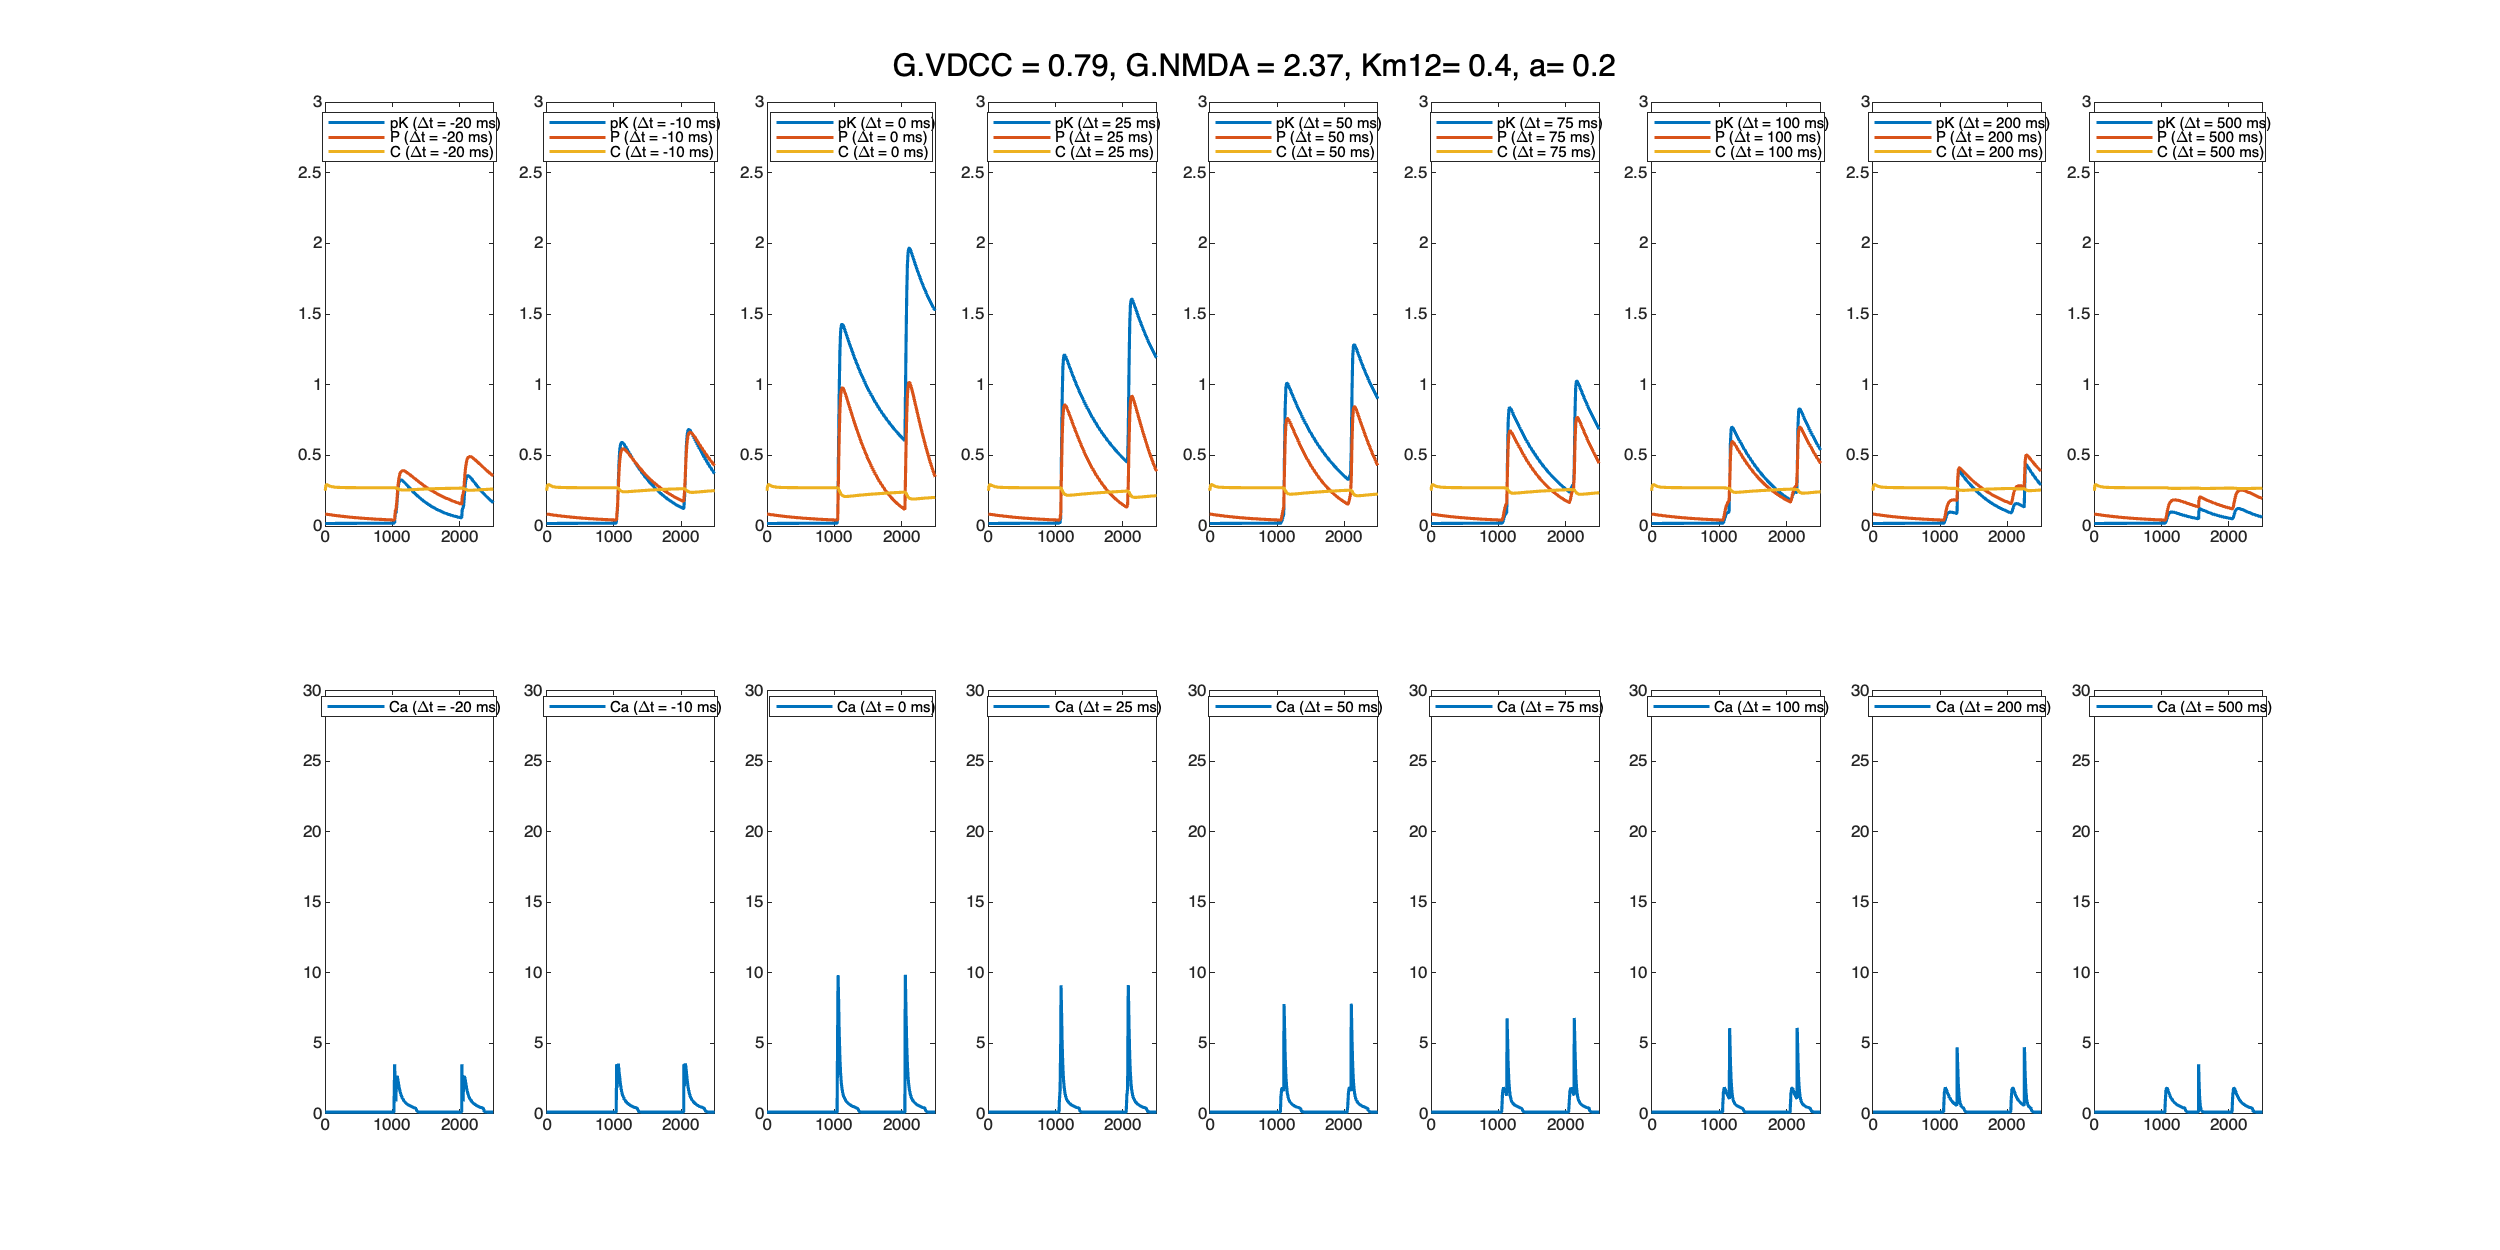
\includegraphics[width=0.8\textwidth]{G_VDCC=0.79_G_NMDA=2.37_Km12=0.400_a=0.20.png} % Change 'a=0.25.png' to your file name
    \captionof{figure}{ \(G_{\text{VDCC}}=0.79,G_{\text{NMDA}}=2.37,Km12=0.400,a=0.20\)}
    \label{fig:a0.25}
\end{minipage}
\begin{minipage}{\textwidth} % Full width for the second plot
    \centering
    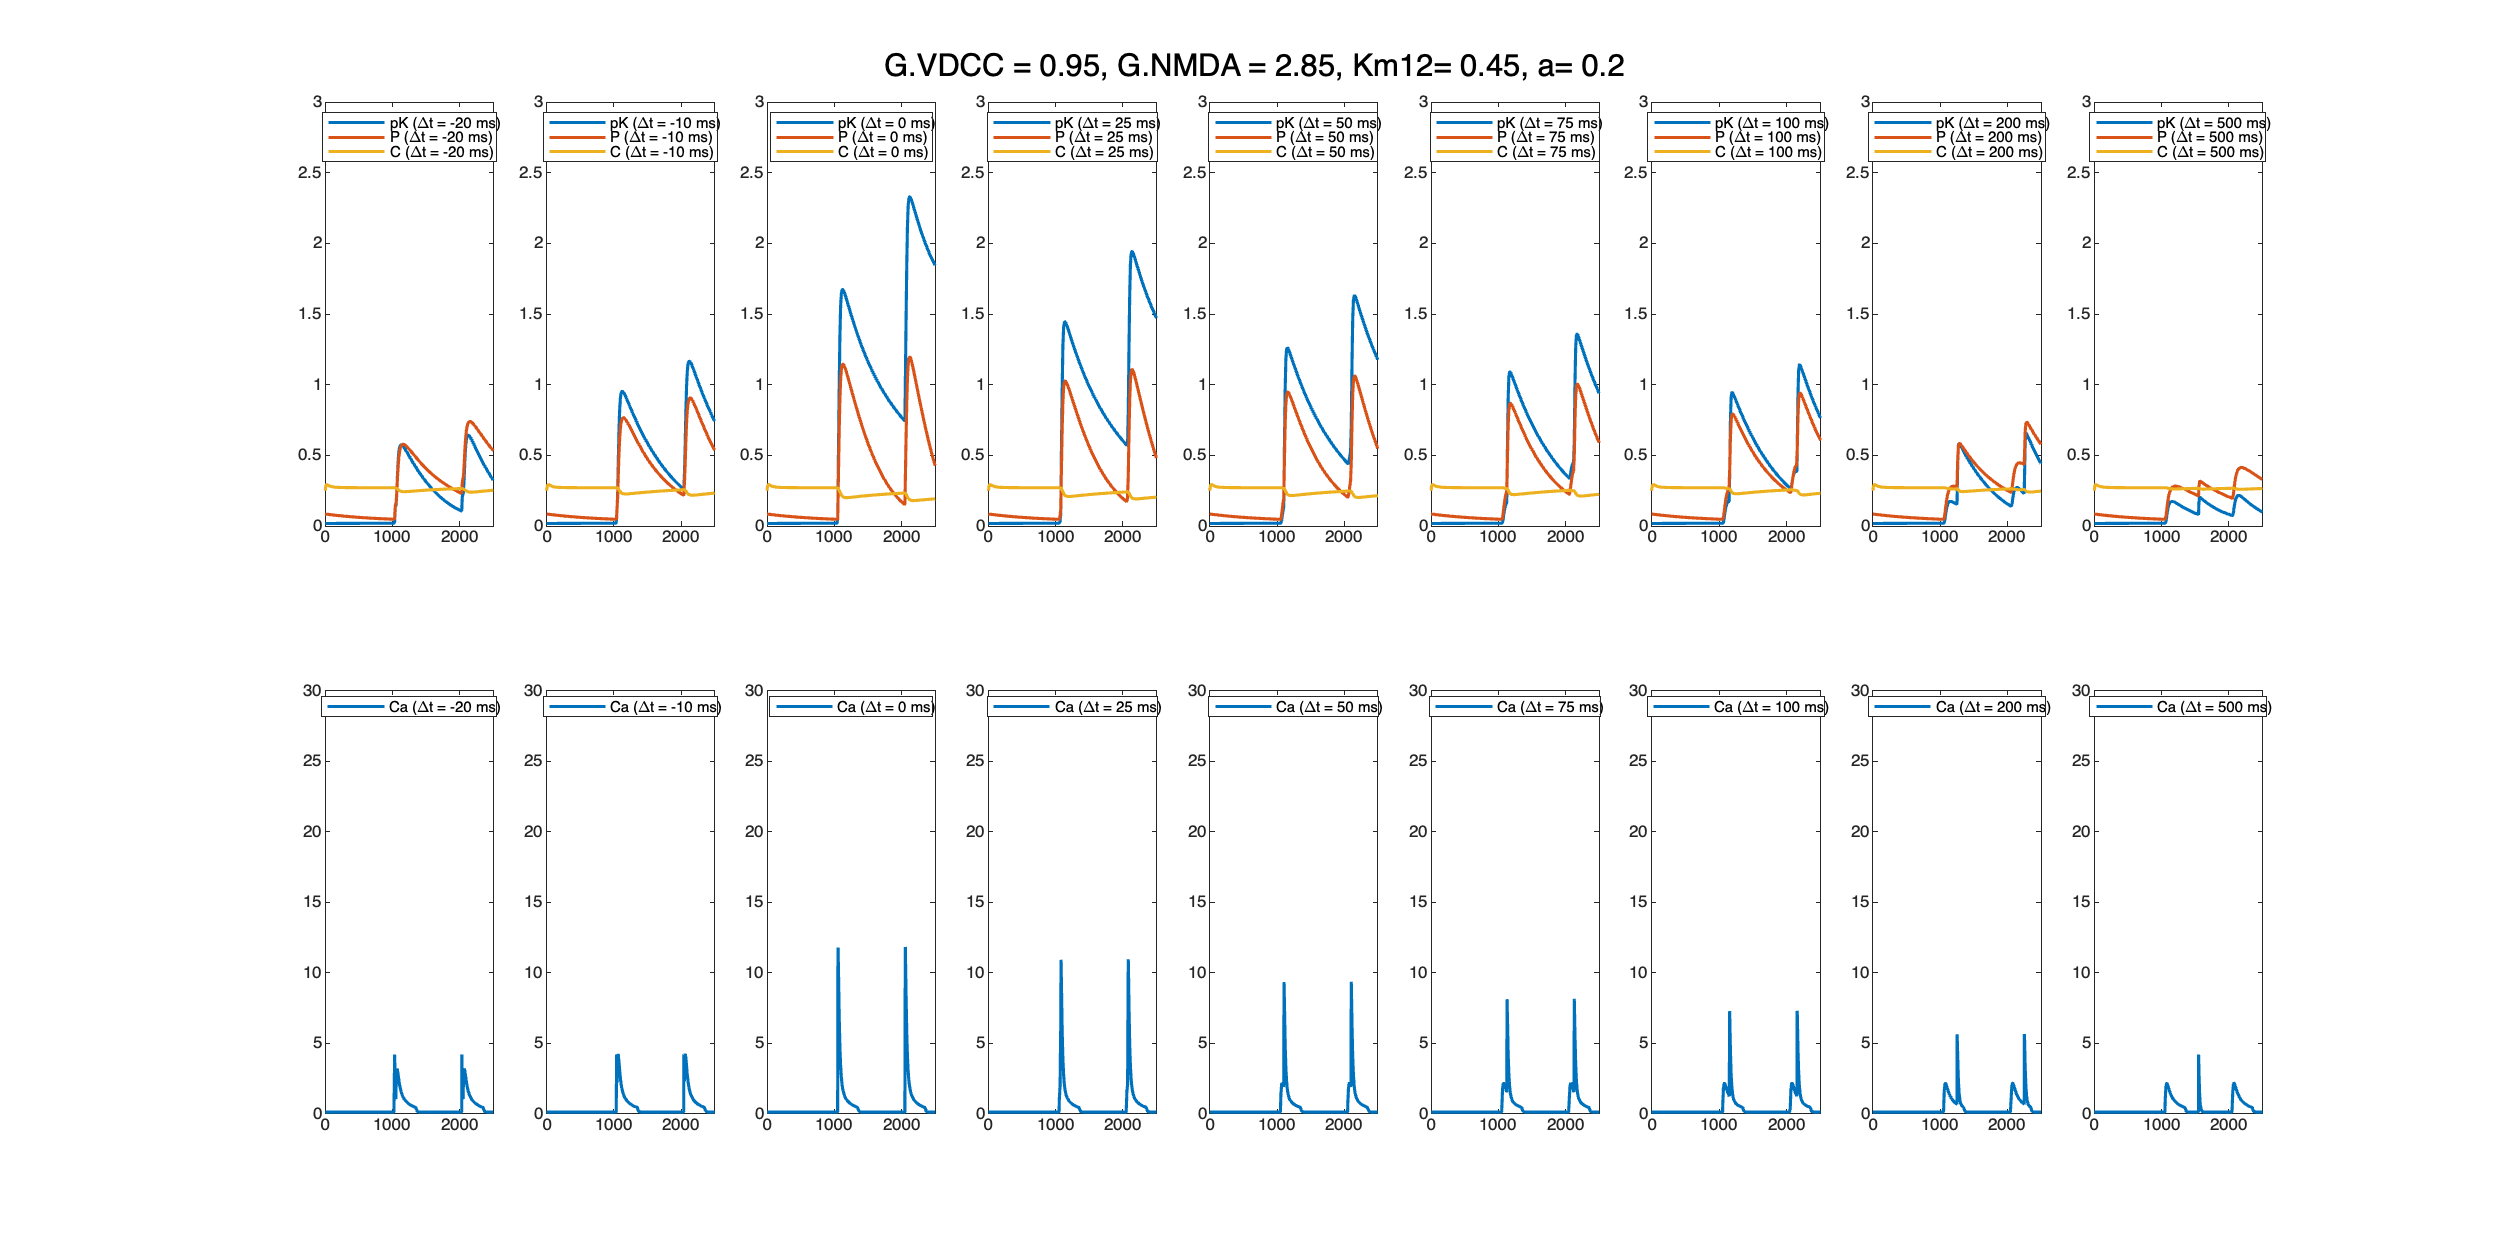
\includegraphics[width=0.8\textwidth]{G_VDCC=0.95_G_NMDA=2.85_Km12=0.450_a=0.20.png} % Change 'a=0.25.png' to your file name
    \captionof{figure}{ \(G_{\text{VDCC}}=0.95,G_{\text{NMDA}}=2.85,Km12=0.450,a=0.20\)}
    \label{fig:a0.25}
\end{minipage}
\begin{minipage}{\textwidth} % Full width for the second plot
    \centering
    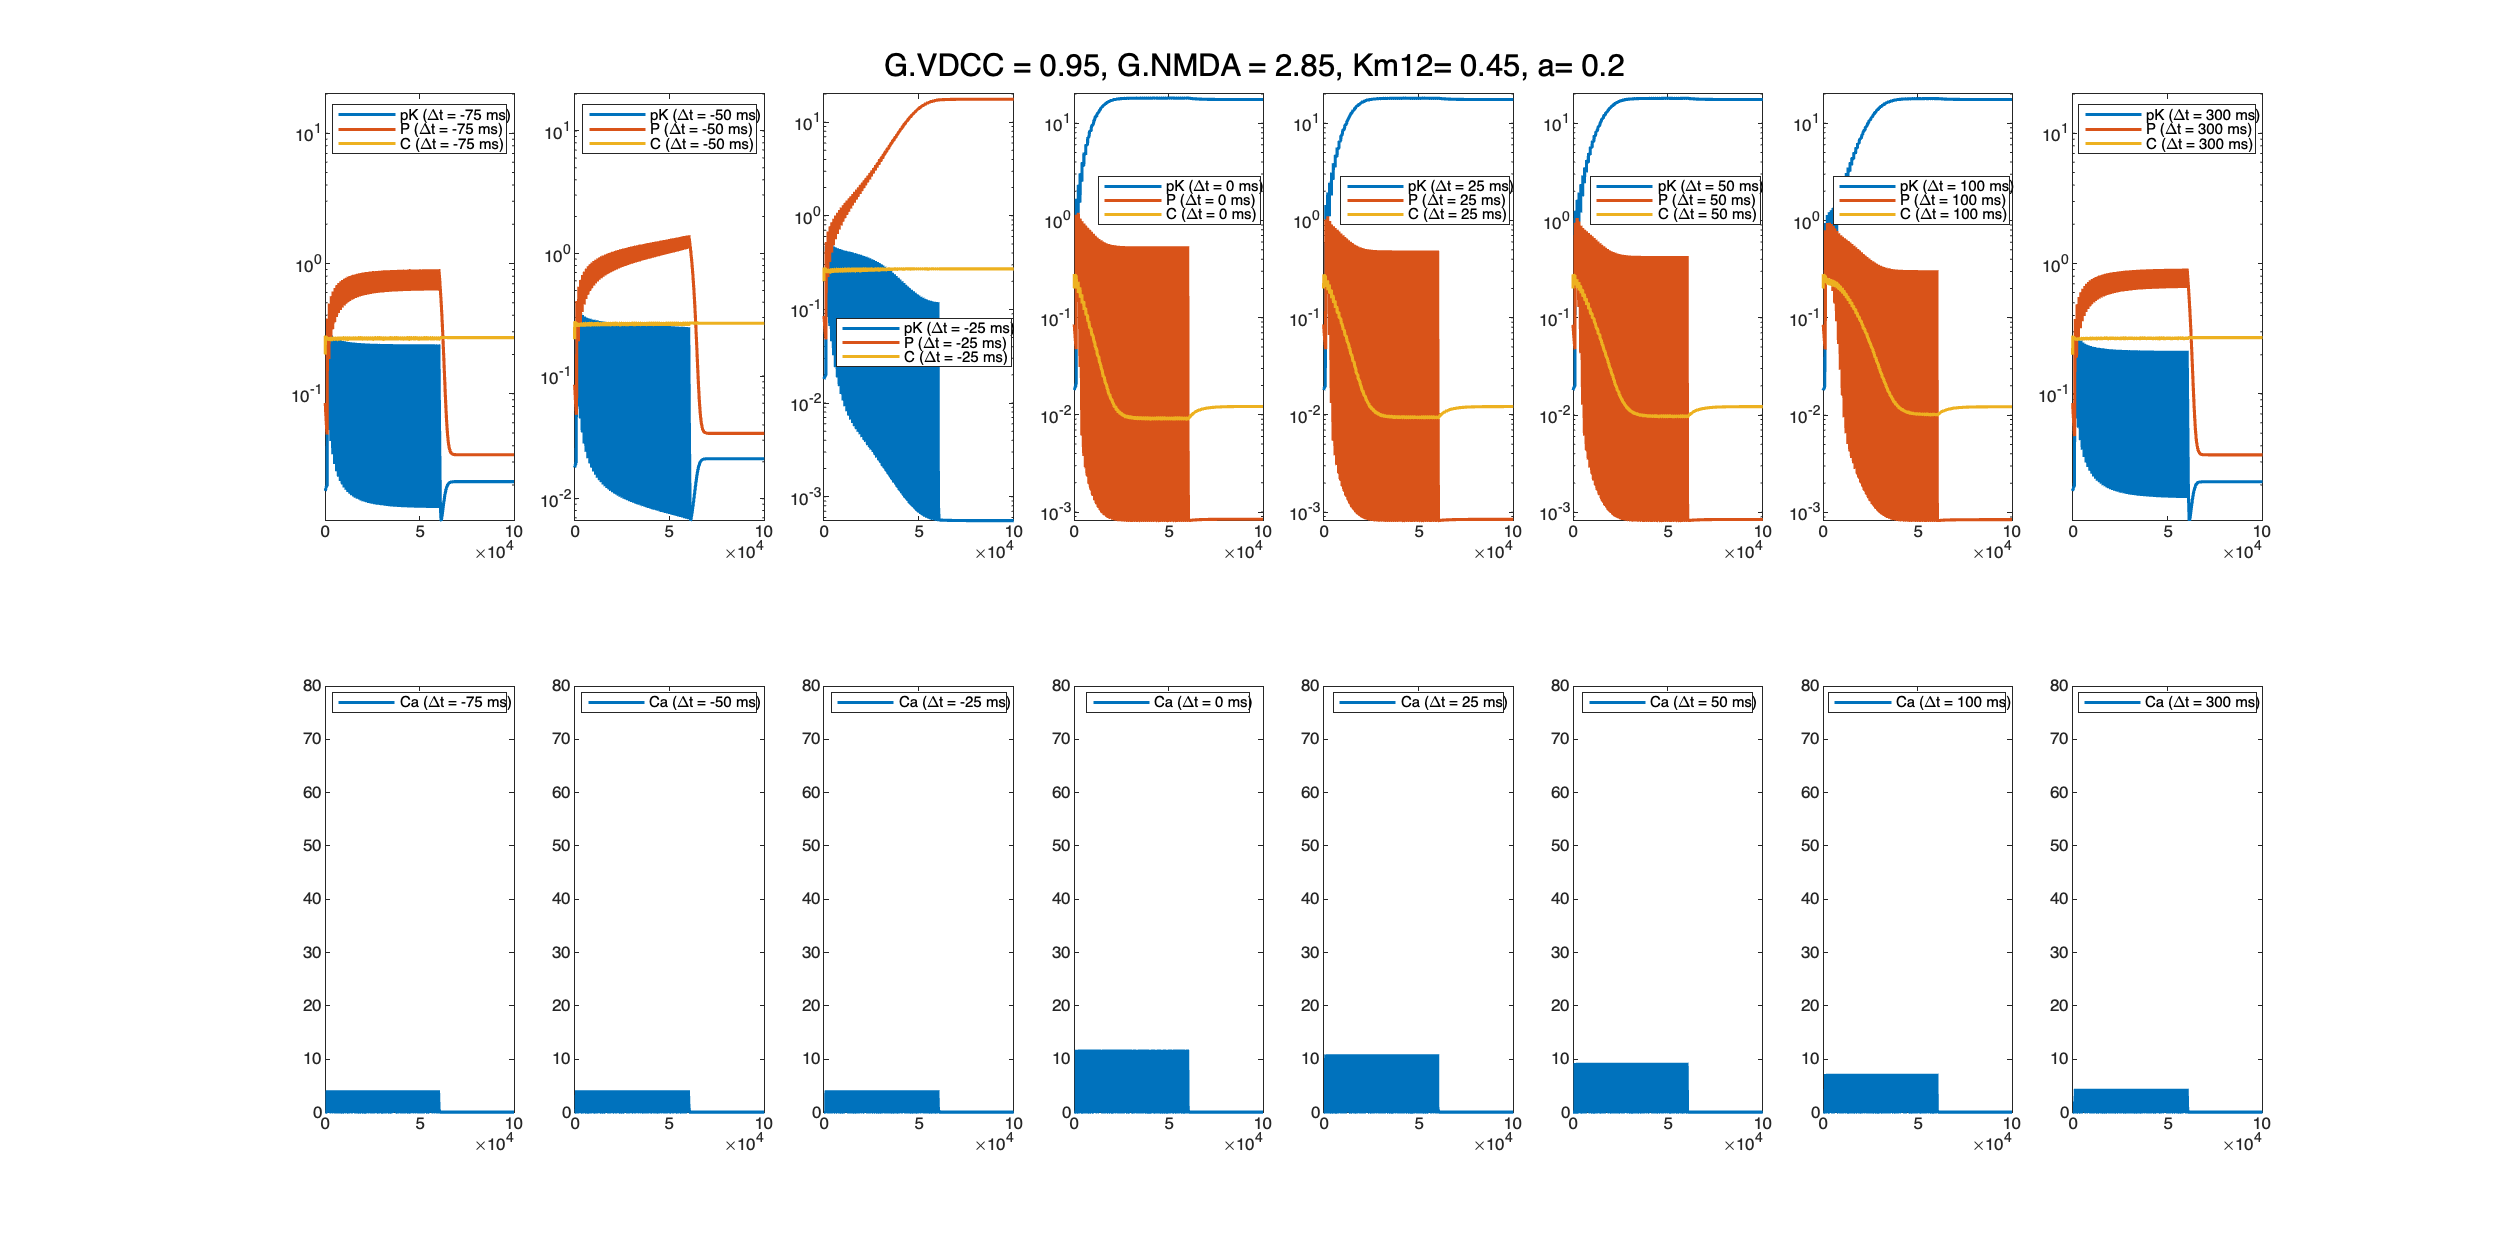
\includegraphics[width=0.8\textwidth]{G_VDCC=0.95_G_NMDA=2.85_Km12=0.450_a=0.20_long.png} % Change 'a=0.25.png' to your file name
    \captionof{figure}{ \(G_{\text{VDCC}}=0.95,G_{\text{NMDA}}=2.85,Km12=0.450,a=0.20\)}
    \label{fig:a0.25}
\end{minipage}
\subsection{ratio of $G_{\text{VDCC}}:G_{\text{NMDA}}$}
We define $\text{ratio}=G_{\text{VDCC}}:G_{\text{NMDA}}$, previously, we set ratio=3. Under this setting, When $\Delta t=500ms$, we have $1:2$ ratio for calcium into NMDAR and VDCC\\
\begin{minipage}{\textwidth} % Full width for the second plot
    \centering
    \includegraphics[width=0.8\textwidth]{1:3.png} % Change 'a=0.25.png' to your file name
    \captionof{figure}{ratio=3}
    \label{fig:a0.25}
\end{minipage}\\
We know that when ratio decrease from 3 into 2 or 1.5, we actualy can observe a smaller ratio for calcium into NMDAR and VDCC(height difference is larger)\\
\begin{figure}[h]
    \centering
    \begin{minipage}[b]{0.45\textwidth}
        \includegraphics[width=1\textwidth]{1:1.5.png}
        \caption{ratio=$1:1.5$}
        \label{fig:image1}
    \end{minipage}
    \hfill % or \hspace*{\fill} to have space between the two figures
    \begin{minipage}[b]{0.45\textwidth}
        \includegraphics[width=\textwidth]{1:2.png}
        \caption{ratio=$1:2$}
        \label{fig:image2}
    \end{minipage}
\end{figure}\\
Therefore, we may be interested in what is the direct consequence of a smaller ratio for calcium into NMDAR and VDCC. In another word, we are interested in how it affect the calcium profile. Here is the result.
\\
\begin{minipage}{\textwidth} % Full width for the second plot
    \centering
    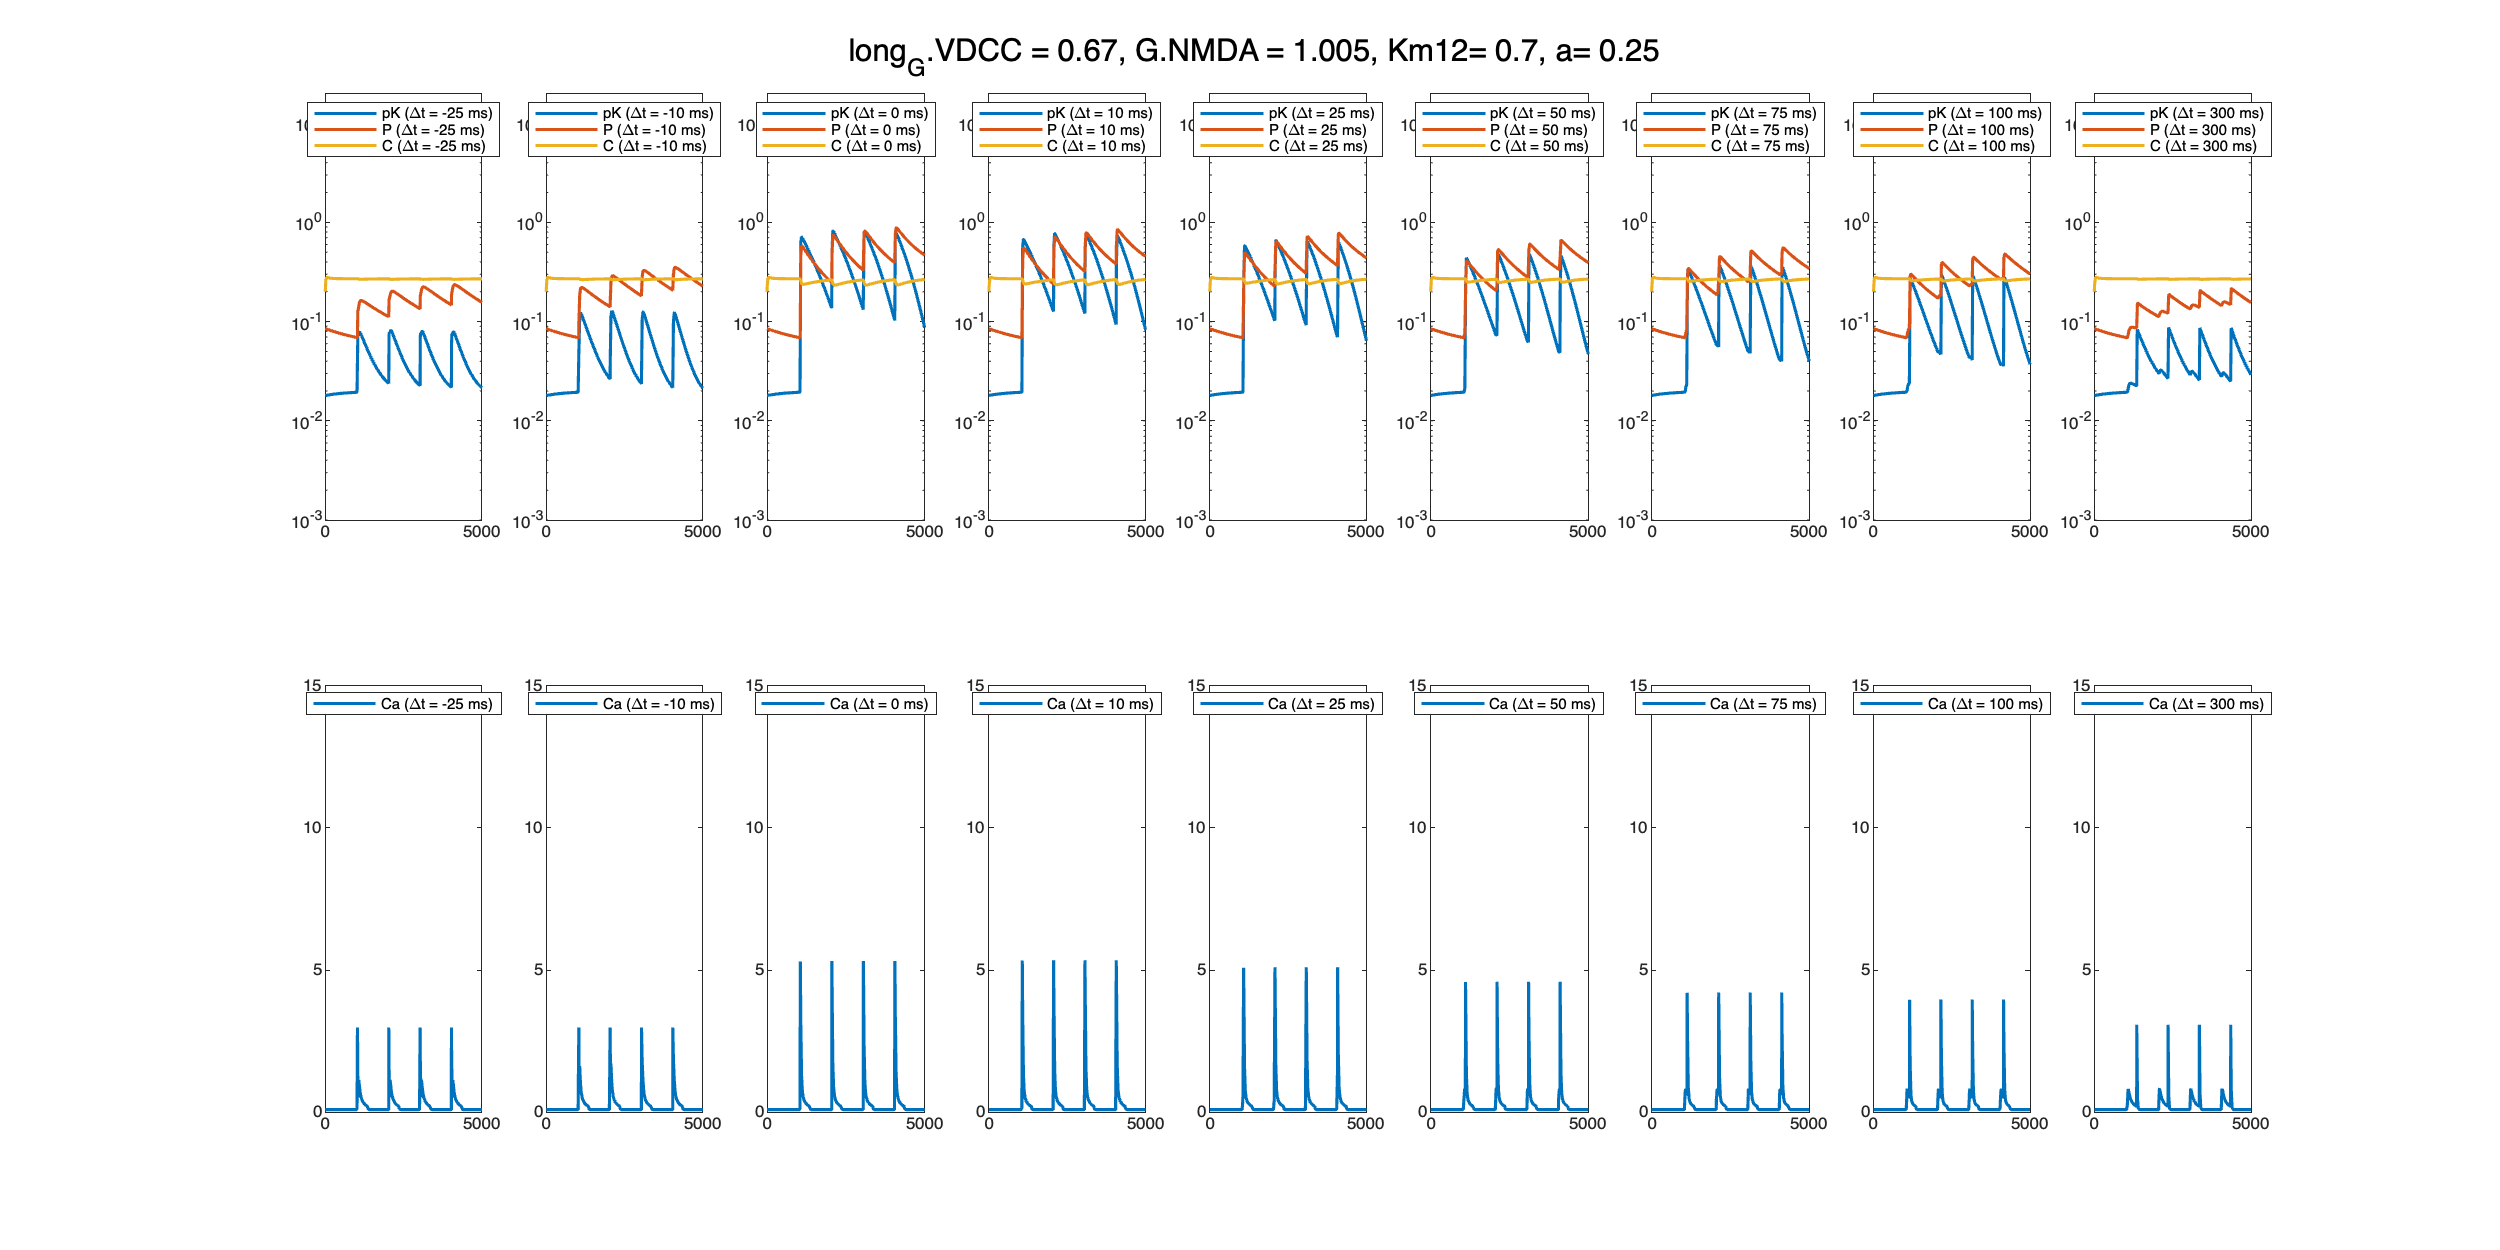
\includegraphics[width=0.8\textwidth]{short_G_VDCC=0.67_G_NMDA=1.00_Km12=0.700_a=0.25.png} % Change 'a=0.25.png' to your file name
    \captionof{figure}{ratio=1.5}
    \label{fig:a0.25}
\end{minipage}
\begin{minipage}{\textwidth} % Full width for the second plot
    \centering
    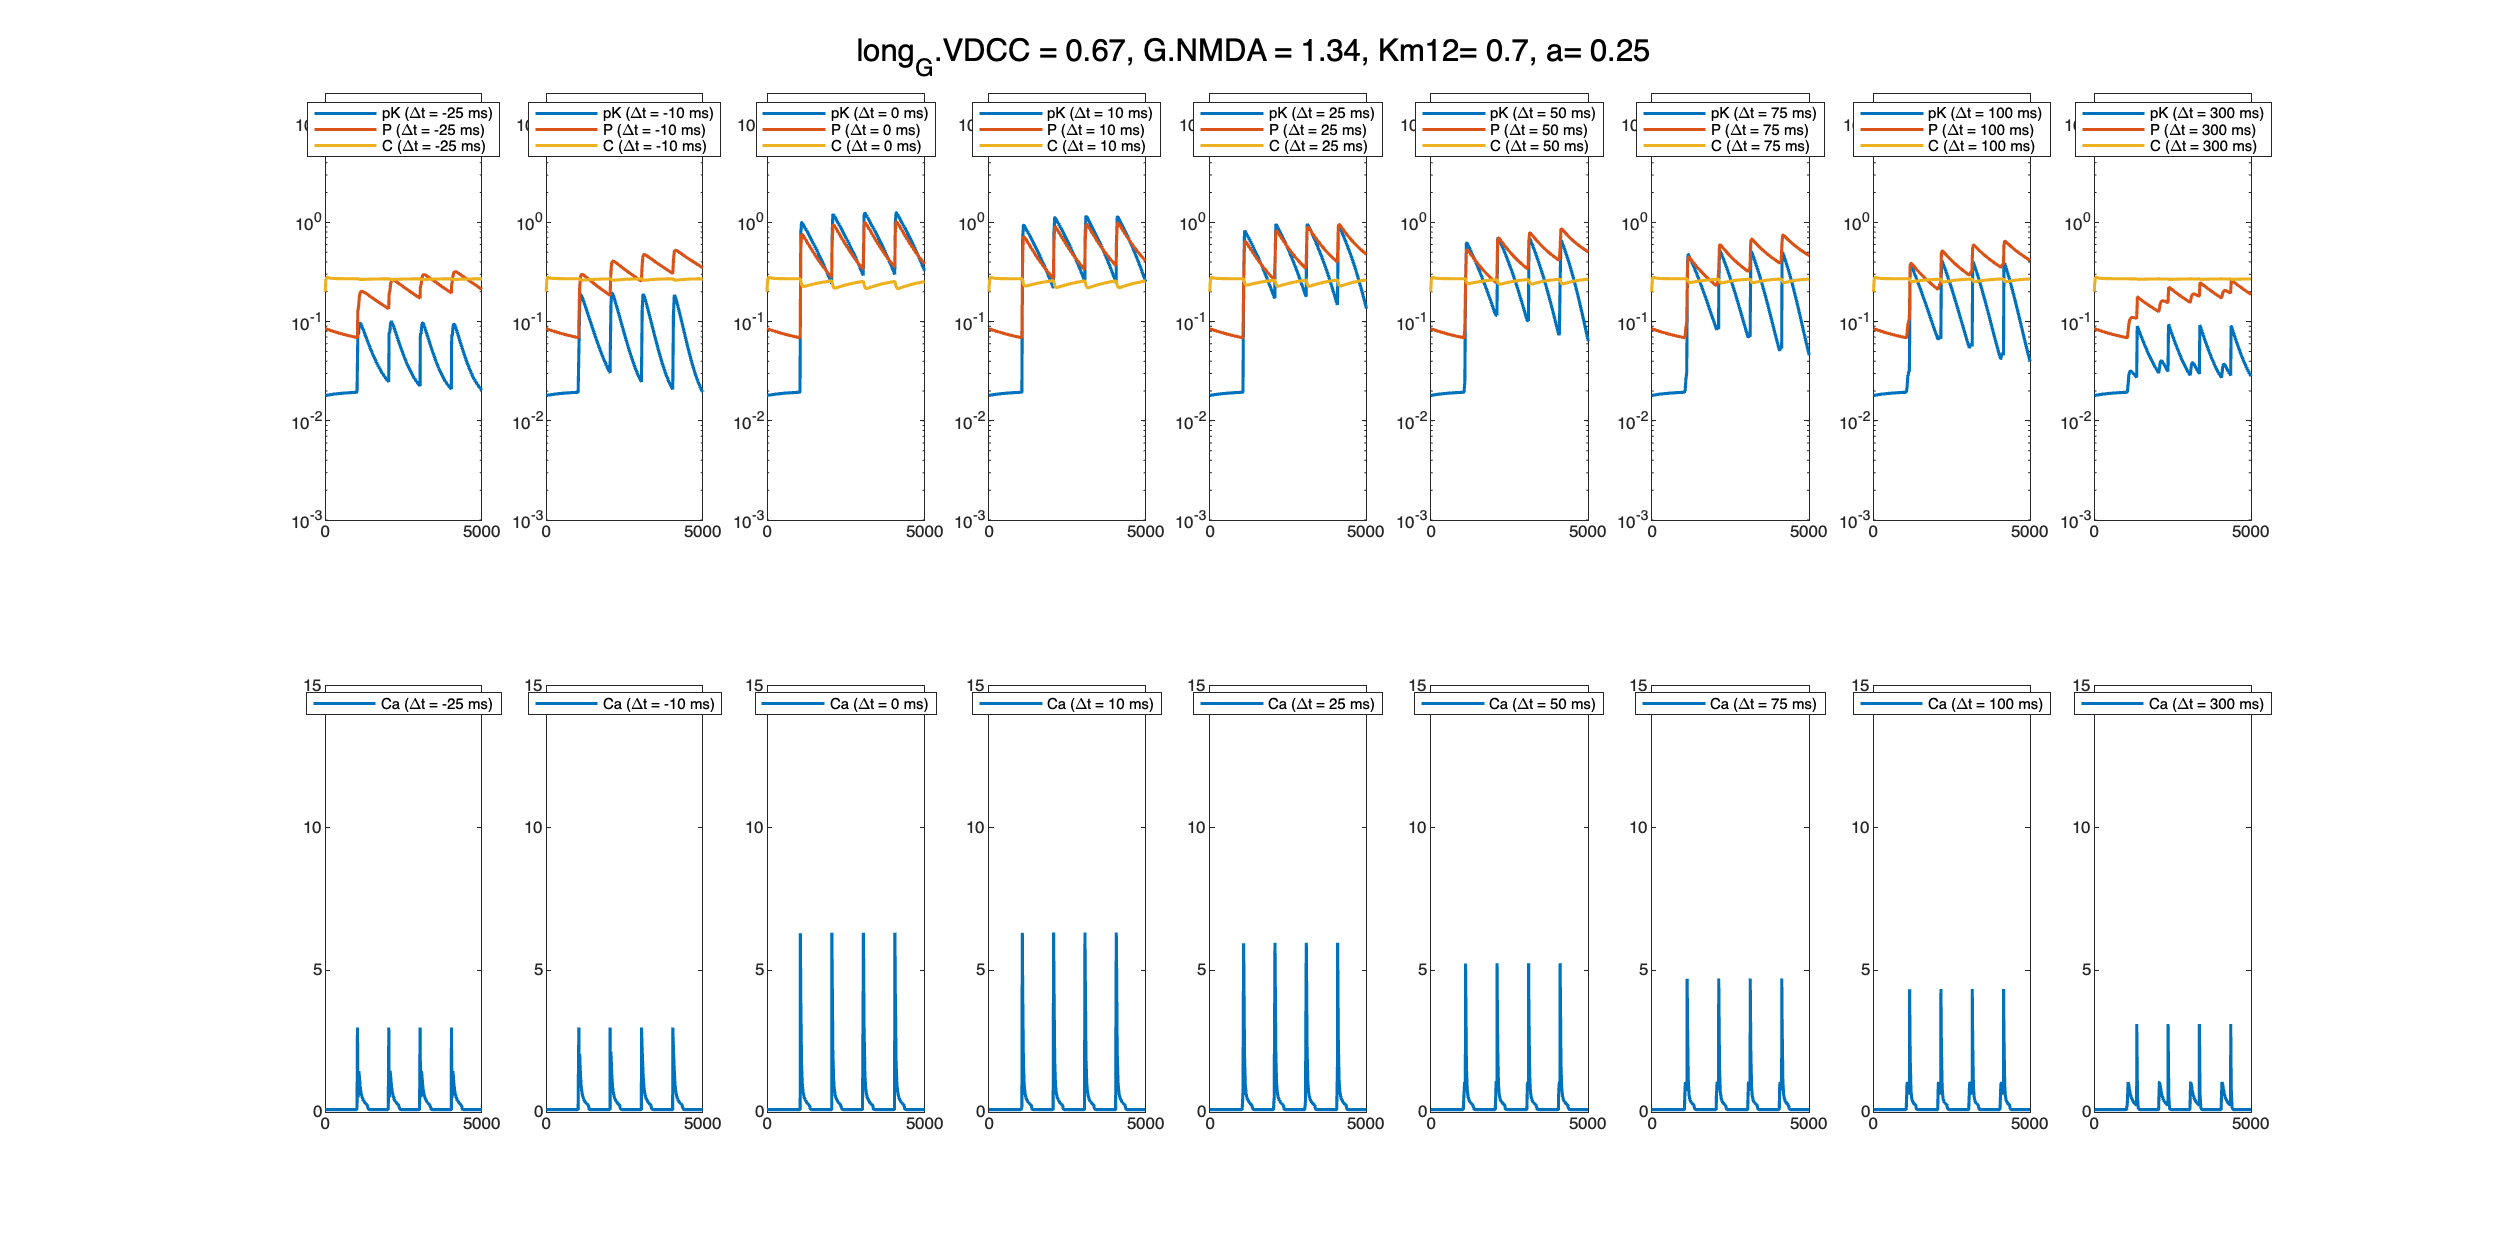
\includegraphics[width=0.8\textwidth]{short_G_VDCC=0.67_G_NMDA=1.34_Km12=0.700_a=0.25.png} % Change 'a=0.25.png' to your file name
    \captionof{figure}{ratio=2}
    \label{fig:a0.25}
\end{minipage}
\begin{minipage}{\textwidth} % Full width for the second plot
    \centering
    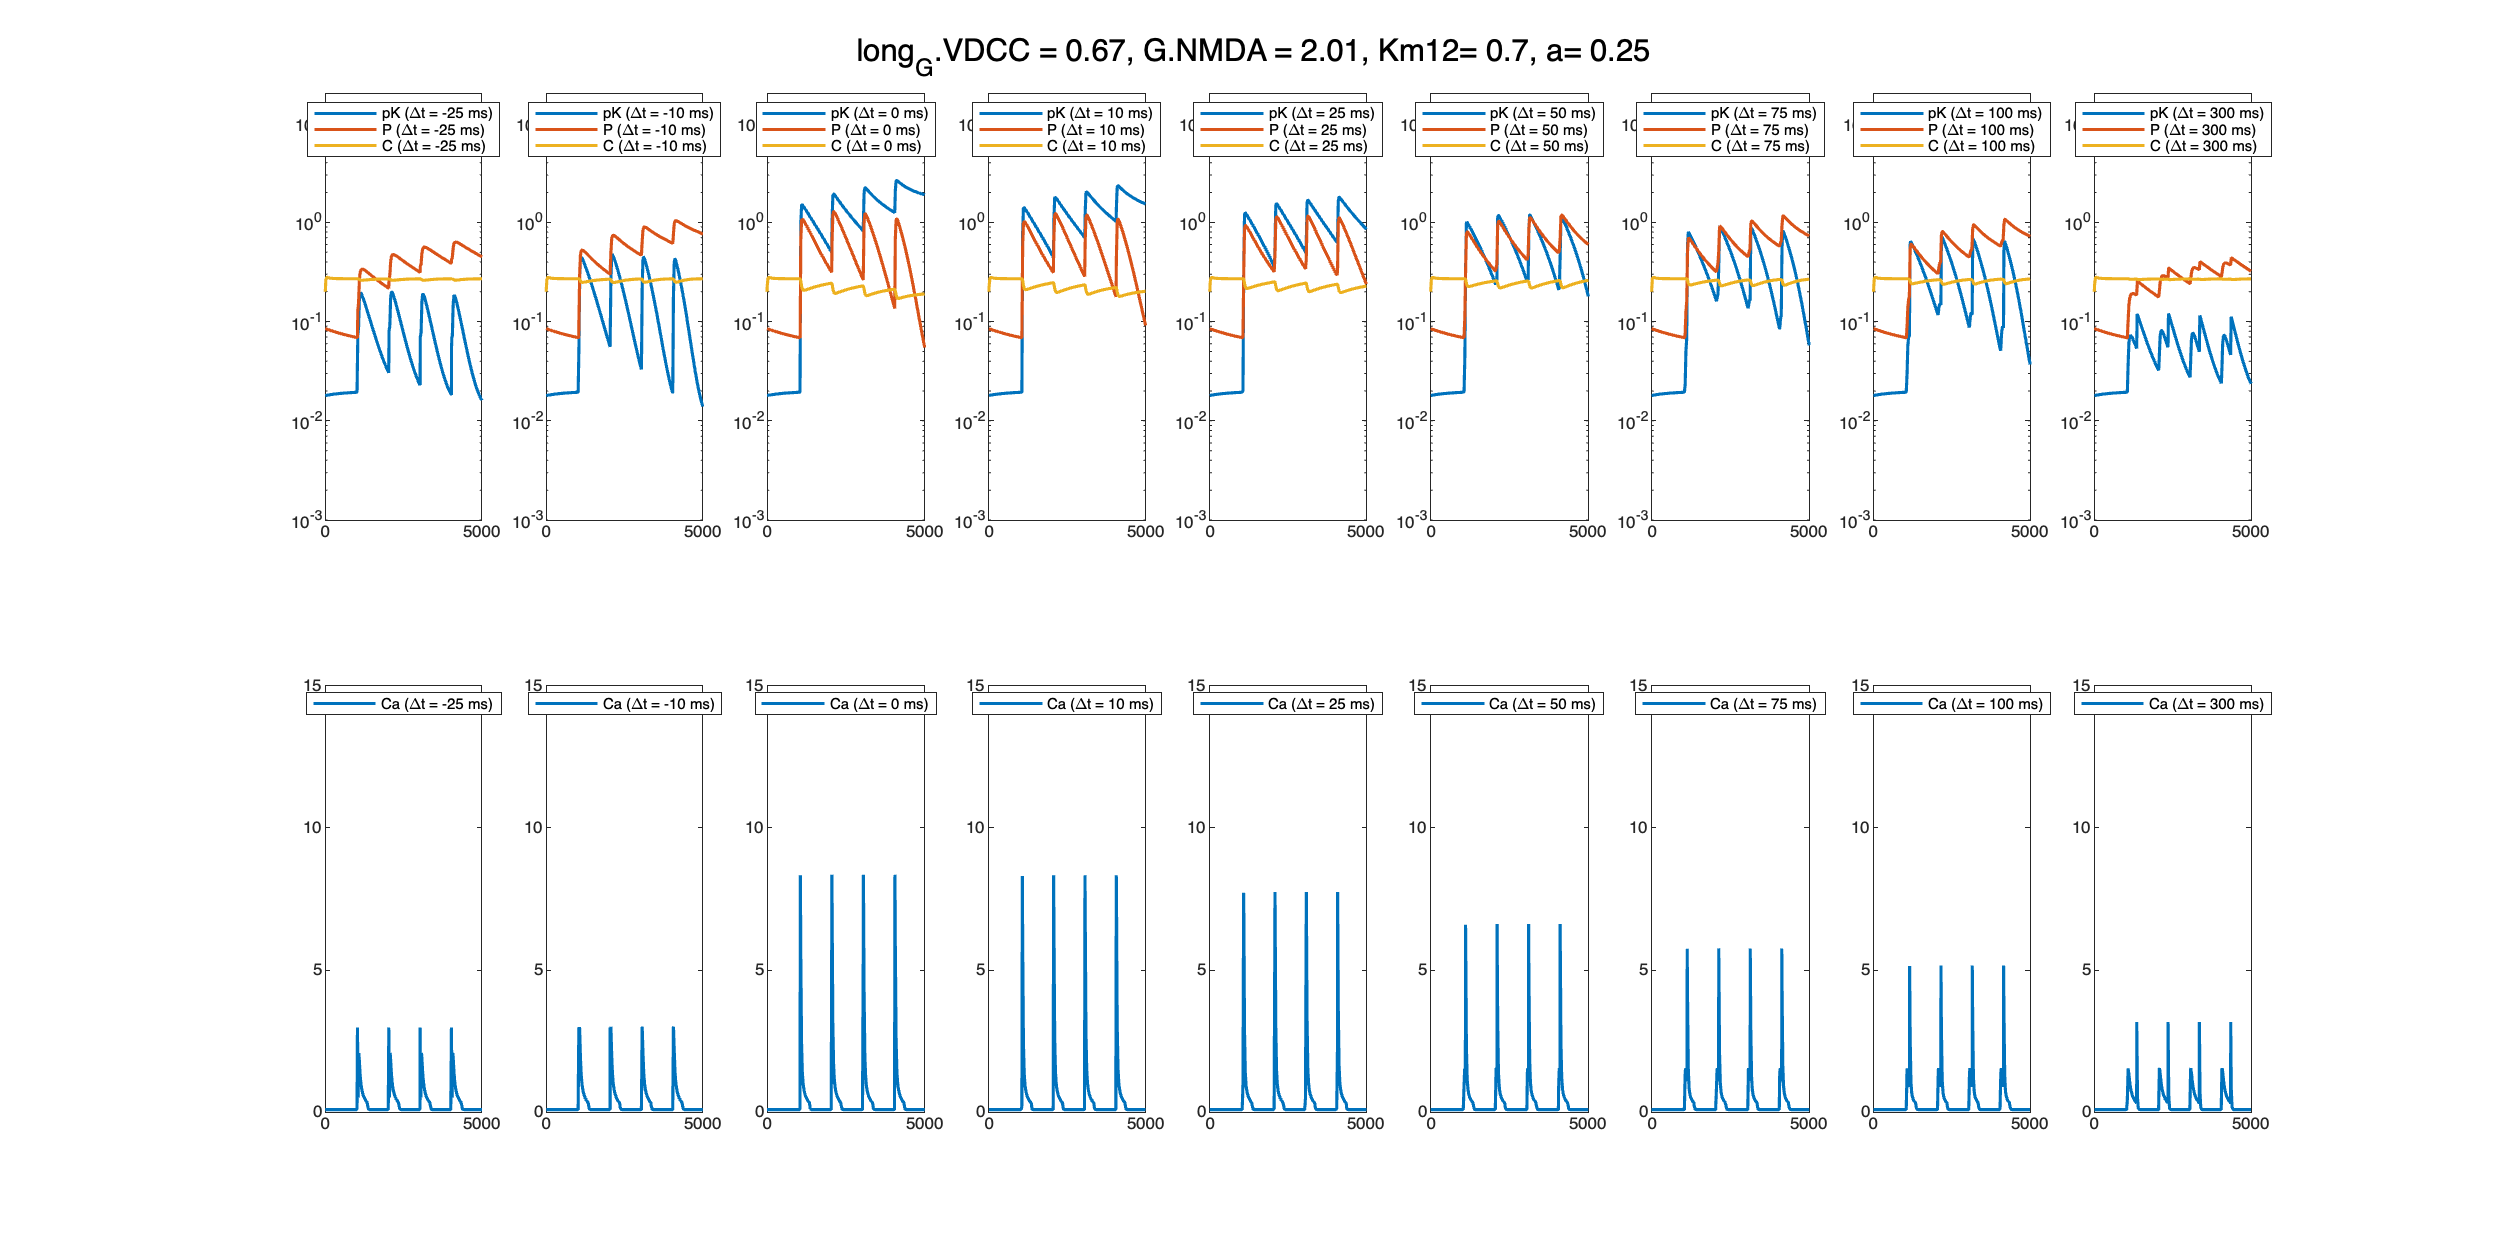
\includegraphics[width=0.8\textwidth]{short_G_VDCC=0.67_G_NMDA=2.01_Km12=0.700_a=0.25.png} % Change 'a=0.25.png' to your file name
    \captionof{figure}{ratio=3}
    \label{fig:a0.25}
\end{minipage}
\\
When ratio become smaller, we find two observation: 1) overall calcium height become smaller, 2) the two jump from for calcium profile (-10 to 0) and (25 to 50) become subtle. The first jump induce LTP from basal, and second jump partially explain the exixtence of "LTD blip".

After varing the ratio, we find a group of result that are interesting. The setting is $a=0.25,km12=0.55,ratio=1.5$. \\
\begin{minipage}{\textwidth} % Full width for the second plot
    \centering
    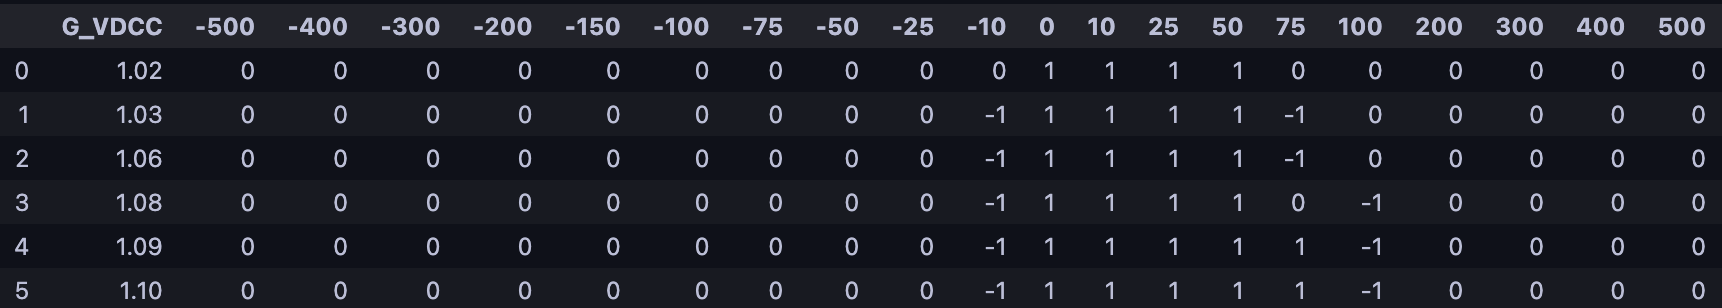
\includegraphics[width=0.8\textwidth]{result1.png} % Change 'a=0.25.png' to your file name
    \captionof{figure}{a=0.25,km12=0.55,ratio=1.5}
    \label{fig:a0.25}
\end{minipage}
The most interesting set is when $G_{\text{VDCC}}=1.08$. In this case, we can actually observe a balanced state at $\Delta t=75$ in the sense that when $\Delta t$ increase, the system drops to basal from LTP, which is what we want. The question remaining is: 1) it goes back to LTD again when $\Delta t=100$. 2) It is in the LTP preferred region. The following color plot can illustrate the second point:
\\
\begin{minipage}{\textwidth} % Full width for the second plot
    \centering
    \includegraphics[width=0.6\textwidth]{a=0.25_final_state_1:1.5.png} % Change 'a=0.25.png' to your file name
    \captionof{figure}{a=0.25,ratio=1.5}
    \label{fig:a0.25}
\end{minipage}\\
To see the first point, here we look into its short run and long run:\\
\begin{minipage}{\textwidth} % Full width for the second plot
    \centering
    \includegraphics[width=0.85\textwidth]{1:1.500000_short_G_VDCC=1.08_G_NMDA=1.62_Km12=0.550_a=0.25.png} % Change 'a=0.25.png' to your file name
    \captionof{figure}{a=0.25,ratio=1.5,short run}
    \label{fig:a0.25}
\end{minipage}\\
\begin{minipage}{\textwidth} % Full width for the second plot
    \centering
    \includegraphics[width=0.85\textwidth]{1:1.500000_long_G_VDCC=1.08_G_NMDA=1.62_Km12=0.550_a=0.25.png} % Change 'a=0.25.png' to your file name
    \captionof{figure}{a=0.25,ratio=1.5,long run}
    \label{fig:a0.25}
\end{minipage}
When we examine the short run, when $\Delta t=75$, this is the desired balanced case in the sense that the decay rate for pK and P match quite well. Both pK and P stimulus is considerable intense compared to $\Delta t=-75$, but two stimulus "cancel" each other, so it goes to back to basal for this case. We believe this is targeted basal that we expect when we want to achieve DP. For the long run plot, we can look into the general shape of case for $\Delta t=75$ and $\Delta t=-75$. Both of them goes to DP, but the trend is different. We can compare it with Guanchun's model's plot as following:\\
\begin{minipage}{\textwidth} % Full width for the second plot
    \centering
    \includegraphics[width=0.9\textwidth]{guanchun's plot.png} % Change 'a=0.25.png' to your file name
    \captionof{figure}{plot in Guanchun's model}
    \label{fig:a0.25}
\end{minipage}
For both large positive/negative $\Delta t$ the long time run is very similar to Guanchun's result, so this may confirm our result here. I think for positive large $\Delta t$'s basal case, the basal is consequence of "competition" from two curve. A difference I observed is that for Guanchun's case, two curve compete for first very few pairs, but i my case, the competition last longer. I am not sure what this can teach us. In any cases, as I mentioned before a little increase on the $\Delta t$ make this basal going to LTD. Also, this balance seems to sensitive to $G_{\text{VDCC}}$: as we can confirm in the read out plot. A tiny variation on $G_{\text{VDCC}}$ make the balance collapse. Also, we should always keep in mind that this is in the LTP preferred region. Therefore, more adjustment is needed on this.

Here I attach the pK-P phase diagram for this parameter setting:\\
\begin{figure}[h]
    \centering
    \begin{minipage}[b]{0.35\textwidth}
        \includegraphics[width=1\textwidth]{phase_diagram_1.png}
        \caption{phase diagram}
        \label{fig:image1}
    \end{minipage}
    \hfill % or \hspace*{\fill} to have space between the two figures
    \begin{minipage}[b]{0.35\textwidth}
        \includegraphics[width=\textwidth]{null_cline_with_vector_field.png}
        \caption{null cline}
        \label{fig:image2}
    \end{minipage}
\end{figure}\\
\subsection{k11 and km11}
We now review our biochemical system defined before:
\begin{equation}
\left\{
    \begin{aligned}
        \frac{d}{dt}pK &= k_1 \frac{K}{K_{m1} + K}pK - k_2 \frac{pK}{K_{m2} + pK}(P + P_0) + k_3K_0 + k_4 \frac{Ca^4}{K_{m4}^4 + Ca^4} K\\
        \frac{d}{dt}P &= k_{11} \frac{pP}{K_{m11} + pP}P - k_{12} \frac{P}{K_{m12} + P}(pK + pK_0) + k_{13}P_0 + k_{14} \frac{Ca^3}{K_{m}^3 + Ca^3}pP,\\
        \frac{dC}{dt} &=-\mu C+\nu K
    \end{aligned}
\right.
\end{equation}

We want to adjust the auto-dephosphorylation effect by linearizing the first term of the equation for \( P \), specifically:
\(
k_{11} \frac{pP}{K_{m11} + pP} P,
\)
where \( P \) is relatively moderate. To achieve this, we propose reducing \( K_{m11} \) to make it effectively smaller. For instance, in the current model where \( P_{\text{tot}} = 20 \, \mu \text{M} \), we set \( K_{m11} = 10 \, \mu \text{M} \) (a 2:1 ratio).

Reducing \( K_{m11} \) inherently increases the value of the first term. Therefore, we must also adjust \( k_{11} \) to maintain the original value of 
\(
k_{11} \frac{pP}{K_{m11} + pP} P,
\)
at the basal steady-state values \( P^* \) and \( pP^* \). This adjustment aims to keep the expression
\(
k_{11} \frac{pP}{K_{m11} + pP} P,
\)
constant across changes to \( K_{m11} \) and \( k_{11} \).


In experiment, we found out that after we decrease km11, we suppose to adjust k11 to maintain first term's quantity unchanged. \textbf{However}, simulation result show that doing so will make the sensitivity of decreasing k11 for the biochemical system become too subtle. In another word, changing k11 will cause no notable difference for the biochemical system. Therefore, we decide to use k11 unchanged all the time indepent from km11's value.

in this section we define ratio $r=\frac{P_{\text{tot}}}{Km11}$.

Here is some plot illustrate how phase diagram respond to different r.
\begin{figure}[h]
    \centering
    \begin{minipage}[b]{0.35\textwidth}
        \includegraphics[width=1\textwidth]{phase_diagram_ratio=2.png}
        \caption{r=2}
        \label{fig:image1}
    \end{minipage}
    \hfill % or \hspace*{\fill} to have space between the two figures
    \begin{minipage}[b]{0.35\textwidth}
        \includegraphics[width=\textwidth]{phase_diagram_ratio=100.png}
        \caption{r=100}
        \label{fig:image2}
    \end{minipage}
\end{figure}\\
Here is some short run respond to different r.\\
\begin{minipage}{\textwidth} % Full width for the second plot
    \centering
    \includegraphics[width=0.9\textwidth]{1:1.500000_short_G_VDCC=1.000_G_NMDA=1.500_Km12=0.700_a=0.25_ratio=2.png} % Change 'a=0.25.png' to your file name
    \captionof{figure}{r=2}
    \label{fig:a0.25}
\end{minipage}
\begin{minipage}{\textwidth} % Full width for the second plot
    \centering
    \includegraphics[width=0.9\textwidth]{1:1.500000_short_G_VDCC=1.000_G_NMDA=1.500_Km12=0.700_a=0.25_ratio=100.png} % Change 'a=0.25.png' to your file name
    \captionof{figure}{r=100}
    \label{fig:a0.25}
\end{minipage}\\
A key observation here is that when p become larger from 2 to 100, the P become more dominant. This can be both seen in short run and phase diagram. We can then check the nullcline plot.
\begin{figure}[h]
    \centering
    \begin{minipage}[b]{0.3\textwidth}
        \includegraphics[width=1\textwidth]{plot_ratio=2.png}
        \caption{r=2}
        \label{fig:image1}
    \end{minipage}
    \hfill % or \hspace*{\fill} to have space between the two figures
    \begin{minipage}[b]{0.3\textwidth}
        \includegraphics[width=\textwidth]{plot_ratio=100.png}
        \caption{r=100}
        \label{fig:image2}
    \end{minipage}
\end{figure}\\
When we see the case for r=100, the blue curve in nullcine plot seems to diverge far from the y-axis. We want its nullcine plot more like the case for r=2. Then, we decrease k11 to 0.06, we get the following nullcine, which is more desired.\\\begin{minipage}{\textwidth} % Full width for the second plot
    \centering
    \includegraphics[width=0.6\textwidth]{plot_k11=0.06.png} % Change 'a=0.25.png' to your file name
    \captionof{figure}{k11=0.06}
    \label{fig:a0.25}
\end{minipage}\\
The short run plot and color plot under this setting is shown here:\\
\begin{minipage}{\textwidth} % Full width for the second plot
    \centering
    \includegraphics[width=0.6\textwidth]{k11=0.060_color.png} % Change 'a=0.25.png' to your file name
    \captionof{figure}{k11=0.06}
    \label{fig:a0.25}
\end{minipage}\\
In $km12=0.9$, it is LTD preferred region, we obtain following long run and short run plot.
\\
\begin{minipage}{\textwidth} % Full width for the second plot
    \centering
    \includegraphics[width=0.8\textwidth]{1:1.500000_short_G_VDCC=1.370_G_NMDA=2.055_Km12=0.900_a=0.25_ratio=100.000000_k11=0.060.png} % Change 'a=0.25.png' to your file name
    \captionof{figure}{k11=0.06 long}
    \label{fig:a0.25}
\end{minipage}\\
\\
\begin{minipage}{\textwidth} % Full width for the second plot
    \centering
    \includegraphics[width=0.8\textwidth]{1:1.500000_short_G_VDCC=1.370_G_NMDA=2.055_Km12=0.900_a=0.25_ratio=100.000000_k11=0.060_short.png} % Change 'a=0.25.png' to your file name
    \captionof{figure}{k11=0.06 short}
    \label{fig:a0.25}
\end{minipage}\\
Here is some observation: for $\Delta t=50ms$, although it goes to LTD, we can see overall two curve in short run balance quite good, but when $\Delta t$ becomes larger the balance collapse. When $\Delta t$ becomes even larger, it goes to basal. What comes to mind is that if we compare previous discussion on the case for balance state before LTD blip occur(figure 49) and Guanchun's plot (figure 50). If we look at the basal state, figure 61 seems have a very short time for competing and directly goes to basal. Guanchun's plot(figure 50) seems have longer time, and the plot (figure 49) have significant longer time for competing of two curve. The point here is that will the competing time crucial for us to erase LTD blip?


\subsection{frequency and pairs}
We are now interested in the following two question: 1)How many pairs of calcium do we need to stimulate LTD/P? 2)How the frequency of calcium impulse will influence the reaction of biochemical system? 

We first take a look at the first question: we fix frequency to be 1 Hz and change pair number\\
\begin{minipage}{\textwidth} % Full width for the second plot
    \centering
    \includegraphics[width=0.8\textwidth]{1:1.500000_short_G_VDCC=1.380_G_NMDA=2.070_Km12=0.900_a=0.25_ratio=100.000000_k11=0.075_pairs=28.000000.png} % Change 'a=0.25.png' to your file name
    \captionof{figure}{28 pairs}
    \label{fig:a0.25}
\end{minipage}\\
\\
\begin{minipage}{\textwidth} % Full width for the second plot
    \centering
    \includegraphics[width=0.8\textwidth]{1:1.500000_short_G_VDCC=1.380_G_NMDA=2.070_Km12=0.900_a=0.25_ratio=100.000000_k11=0.075_pairs=27.000000.png} % Change 'a=0.25.png' to your file name
    \captionof{figure}{27 pairs}
    \label{fig:a0.25}
\end{minipage}\\
\\
\begin{minipage}{\textwidth} % Full width for the second plot
    \centering
    \includegraphics[width=0.8\textwidth]{1:1.500000_short_G_VDCC=1.380_G_NMDA=2.070_Km12=0.900_a=0.25_ratio=100.000000_k11=0.075_pairs=26.000000.png} % Change 'a=0.25.png' to your file name
    \captionof{figure}{26 pairs}
    \label{fig:a0.25}
\end{minipage}\\
In this group of plot, when number of pairs=28, it is standard DPD. When it becomes 27 pairs, LTD at negative side first disappear. And when it decreases to 26 pairs, LTD at positive side disappear as well. That means LTD at positive side require more pairs to stimulate. 

There is an observation here: If we compare figure 65 and 66 and focus on $\Delta t=-10$. In this case, one is LTD and one is basal. My point here is that actually the calcium profile, in terms of height, is very similar, but one more pairs cause them to become LTD. If there is any chance that we need to consider another question: Instead of fixing DPD, we fix 'P'(for example figure 65) in the sense that make basal state for small negative $\Delta t$ to become LTD. I may be wrong here...

Then, we move forward to the next question for frequency. We fix the pairs number to be 60, and decrease frequency by 1
\\
\begin{minipage}{\textwidth} % Full width for the second plot
    \centering
    \includegraphics[width=0.8\textwidth]{pairs=60_hertz=0.70.png} % Change 'a=0.25.png' to your file name
    \captionof{figure}{0.7 Hz}
    \label{fig:a0.25}
\end{minipage}\\
\\
\begin{minipage}{\textwidth} % Full width for the second plot
    \centering
    \includegraphics[width=0.8\textwidth]{pairs=60_hertz=0.65.png} % Change 'a=0.25.png' to your file name
    \captionof{figure}{0.65 Hz}
    \label{fig:a0.25}
\end{minipage}\\
\\
\begin{minipage}{\textwidth} % Full width for the second plot
    \centering
    \includegraphics[width=0.8\textwidth]{pairs=60_hertz=0.60.png} % Change 'a=0.25.png' to your file name
    \captionof{figure}{0.6 Hz}
    \label{fig:a0.25}
\end{minipage}\\
One takeaway here may be when frequency become smaller, it is harder for LTD at negative side to be observed.
\subsection{pre}
\begin{equation}
\left\{
    \begin{aligned}
        \frac{d}{dt}pK &= k_1 \frac{K}{K_{m1} + K}pK - k_2 \frac{pK}{K_{m2} + pK}(P + P_0) + k_3K_0 + k_4 \frac{Ca^4}{K_{m4}^4 + Ca^4} K\\
        \frac{d}{dt}P &= k_{11} \frac{pP}{K_{m11} + pP}P - k_{12} \frac{P}{K_{m12} + P}(\text{pre}\cdot pK + pK_0) + k_{13}P_0 + k_{14} \frac{Ca^3}{K_{m}^3 + Ca^3}pP,\\
        \frac{dC}{dt} &=-\mu C+\nu K
    \end{aligned}
\right.
\end{equation}


\newpage
\section{References}
\begin{enumerate}

    \item Carlson, K. D., \& Giordano, N. (2011). Interplay of the magnitude and time-course of postsynaptic Ca\textsuperscript{2+} concentration in producing spike timing-dependent plasticity. \emph{Journal of Computational Neuroscience, 30}, 747-758.
    \item Pi, H. J., \& Lisman, J. E. (2008). Coupled Phosphatase and Kinase Switches Produce the Tristability Required for Long-Term Potentiation and Long-Term Depression. \emph{The Journal of Neuroscience, 28}(49), 13132–13138.
    \item Bi, G.-q., \& Poo, M.-m. (1998). Synaptic Modifications in Cultured Hippocampal Neurons: Dependence on Spike Timing, Synaptic Strength, and Postsynaptic Cell Type. \emph{The Journal of Neuroscience}.
    \item Graupner, M., \& Brunel, N. (2012). Calcium-based plasticity model explains sensitivity of synaptic changes to spike pattern, rate, and dendritic location. \emph{PNAS, 109}(10), 3993.
    \item Li, G., McLaughlin, D. W., \& Peskin, C. S. A Biochemical Description of Postsynaptic Plasticity – with Timescales Ranging from Milliseconds to Seconds.
    
\end{enumerate} 




\end{document}
